\documentclass{article} % For LaTeX2e
\usepackage{iclr2027_conference,times}
\usepackage{enumitem}

% GLOSSARIES
\usepackage[acronym]{glossaries}
% uncomment the below line only if you plan to use \printglossaries somewhere in your text.
\makeglossaries

% MATH
\usepackage{amsmath}
\usepackage{amssymb}
\usepackage{amsthm}
\usepackage{dsfont}
\usepackage{mathtools}
\allowdisplaybreaks

% FIGURES
\usepackage{graphicx}
\usepackage{wrapfig}

% TABLES
\usepackage{booktabs}
\usepackage{caption}

% MISC (must go before hyperref/cleveref)
\usepackage{xcolor}
\usepackage{parskip} % helps with indenting and paragraph layout
% \usepackage[ruled,vlined]{algorithm2e}
\usepackage{soul} % use \ul to underline, fixes wrapping issues

% REFERENCES
% \usepackage[round]{natbib}
% \bibliographystyle{apalike}
\usepackage{hyperref}
\hypersetup{
  colorlinks=true,
  linkcolor=blue,
  citecolor=blue,
  urlcolor=blue
}

\usepackage{enumitem}

\usepackage[capitalise,noabbrev]{cleveref}
% \usepackage{algorithm}
% \usepackage{algpseudocode}


% VERBATIM
\definecolor{midnightblue}{rgb}{0.1, 0.1, 0.44}
\definecolor{mahogany}{rgb}{0.75, 0.25, 0.0}
\definecolor{deltagreen}{RGB}{34,139,34}

\usepackage{listings}
\usepackage{fancyvrb}
\fvset{fontsize=\normalsize}
\newcommand{\red}[1]{\textcolor{BrickRed}{#1}}
\newcommand{\orange}[1]{\textcolor{BurntOrange}{#1}}
\newcommand{\green}[1]{\textcolor{OliveGreen}{#1}}
\newcommand{\blue}[1]{\textcolor{MidnightBlue}{#1}}
\newcommand{\mahogany}[1]{\textcolor{mahogany}{#1}}
\newcommand{\gray}[1]{\textcolor{black!60}{#1}}
\lstdefinestyle{mystyle}{
    commentstyle=\color{OliveGreen},
    keywordstyle=\color{BurntOrange},
    numberstyle=\tiny\color{black!60},
    stringstyle=\color{MidnightBlue},
    basicstyle=\ttfamily,
    breakatwhitespace=false,
    breaklines=true,
    captionpos=b,
    keepspaces=true,
    numbers=left,
    numbersep=5pt,
    showspaces=false,
    showstringspaces=false,
    showtabs=false,
    tabsize=2
}
\lstset{style=mystyle}

% GRAPHICS
\usepackage{tikz}
\usetikzlibrary{shapes,decorations,arrows,calc,arrows.meta,fit,positioning}
\tikzset{
    -Latex,auto,node distance =1 cm and 1 cm,semithick,
    state/.style ={circle, draw, minimum width = 0.7 cm},
    detstate/.style ={rectangle, draw, minimum width = 0.7 cm, minimum height = 0.7 cm},
    point/.style = {circle, draw, inner sep=0.04cm,fill,node contents={}},
    bidirected/.style={Latex-Latex,dashed},
    el/.style = {inner sep=2pt, align=left, sloped}
}
\usepackage[algoruled, algo2e]{algorithm2e}
\usepackage{algorithm}
\usepackage{algorithmic}

%%%%% NEW MATH DEFINITIONS %%%%%
\newcommand{\pdata}{p_{\text{data}}}
\newcommand{\qdata}{q_{\text{data}}}
\newcommand{\pfk}[1]{p_{\textsc{fk}, #1}}

\newcommand{\kl}[1]{\textsc{KL}\!\left(#1\right)}
\newcommand{\D}[1]{\mathcal{D}\left(#1\right)}
\newcommand{\g}{\,|\,}
\newcommand{\lct}{\mathcal{L}_{\textsc{CT-elbo}}}

\newcommand{\ptarget}{p_\text{target}}
\newcommand{\qunsafe}{q_\text{unsafe}}

\newcommand{\expo}[1]{
e^{#1}
}




\def\rvyh{\widehat{\mathbf{y}}}

% THEOREMS AND PROOFS
\newtheorem{assumption}{Assumption}
\newtheorem*{assumption*}{Assumption}
\newtheorem{corollary}{Corollary}
\newtheorem*{corollary*}{Corollary}
\newtheorem{definition}{Definition}
\newtheorem*{definition*}{Definition}
\newtheorem{lemma}{Lemma}
\newtheorem*{lemma*}{Lemma}
\newtheorem{proposition}{Proposition}
\newtheorem*{proposition*}{Proposition}
\newtheorem{theorem}{Theorem}
\newtheorem*{theorem*}{Theorem}

% DEFINITIONS
\DeclareMathOperator*{\argmax}{arg\,max}
\DeclareMathOperator*{\argmin}{arg\,min}
\newcommand{\DKL}{D_{\mathrm{KL}}}
\newcommand{\KL}{\mathrm{KL}}
\DeclareRobustCommand{\wass}[2]{\ensuremath{\mathcal{W}_1\left(#1\;\left.\right\|\;#2\right)}}
\DeclareRobustCommand{\dho}[2]{\ensuremath{\frac{\partial #1}{\partial #2}}}
\renewcommand{\mid}{~\vert~}
% \newcommand{\g}{\,|\,}
\newcommand{\indep}{\,\rotatebox[origin=c]{90}{$\models$}\,}
\newcommand{\nindep}{\,\rotatebox[origin=c]{90}{$\not\models$}\,}
\newcommand{\dif}{\mathop{}\!\mathrm{d}}
\newcommand{\diag}{\textrm{diag}}
\newcommand{\supp}{\textrm{supp}}
\newcommand{\Gam}{\textrm{Gam}}
\newcommand{\InvGam}{\textrm{InvGam}}
\newcommand{\norm}[1]{\left\lVert#1\right\rVert}
\newcommand{\Func}{\mathcal{F}}
\newcommand{\Ker}{\mathcal{K}}
\newcommand{\St}{\mathcal{S}}
\newcommand{\Kernel}{\mathcal{K}_{k}}
\newcommand{\euclid}{\mathbb{R}}
\newcommand{\score}{s^{p}}
\newcommand{\DO}{\text{do}}
\newcommand{\ve}{{\mathtt{\epsilon}}}
\newcommand{\va}{\mathtt{a}}
\newcommand{\vz}{\mathtt{z}}
\newcommand{\vx}{\mathtt{x}}
\newcommand{\vy}{\mathtt{y}}
\newcommand{\vg}{\mathtt{g}}
\newcommand{\vt}{\mathtt{t}}
\newcommand{\gvt}{g(\mathtt{t})}
\newcommand{\Hb}{\mathbf{H}}
\newcommand{\MI}{\mathbf{I}}
\newcommand{\mbeps}{\mbepsilon}
\DeclareRobustCommand{\doot}[1]{\text{do}(\mbt=#1)}
\newcommand{\dinv}{d^{-1}}
\newcommand{\partialder}[2]{\frac{\partial #1}{\partial #2}}
\newcommand{\ind}{\mathbf{1}}
\newcommand{\mbxp}{{\mbx^\prime}}
\newcommand{\xp}{{x^\prime}}
\newcommand{\ince}{\mbI_{NCE}}
\newcommand{\ptr}{{p_{tr}}}
\newcommand{\pte}{{p_{te}}}
\newcommand{\pind}{{p_{\scaleto{\indep}{4pt}}}}
\newcommand{\pindprime}{{p^\prime_{\scaleto{\indep}{4pt}}}}
\newcommand{\varqa}{\sigma^2_{q_a}}
\newcommand{\varqb}{\sigma^2_{q_b}}
\newcommand{\meanqa}{\E_{q_a}}
\newcommand{\meanqb}{\E_{q_b}}
\newcommand{\var}{\text{var}}
\newcommand{\aprime}{{ ( 1 + a)}}
\newcommand{\aminus}{{ ( 1-a)}}
\newcommand{\bprime}{{(1 + b)}}
\newcommand{\bminus}{{ (1 - b)}}
\newcommand{\ruv}{r_{u,v}}
\newcommand{\pinda}{{p_{\scaleto{\indep}{4pt},1}}}
\newcommand{\pindb}{{p_{\scaleto{\indep}{4pt},2}}}
\newcommand{\perf}{\mathtt{Perf}}
\newcommand{\perfte}{\perf_\pte}
\newcommand{\sumybin}{\sum_{y\in \{0,1\}}}
\newcommand{\epsdiff}{\mbeps_2 -\mbeps_1}
\newcommand{\epssum}{\mbeps_1 + \mbeps_2}
\newcommand{\variance}{\sigma^2}

% MATHBF
\newcommand{\mba}{\mathbf{a}}
\newcommand{\mbb}{\mathbf{b}}
\newcommand{\mbc}{\mathbf{c}}
\newcommand{\mbd}{\mathbf{d}}
\newcommand{\mbe}{\mathbf{e}}
\newcommand{\mbg}{\mathbf{g}}
\newcommand{\mbh}{\mathbf{h}}
\newcommand{\mbi}{\mathbf{i}}
\newcommand{\mbj}{\mathbf{j}}
\newcommand{\mbk}{\mathbf{k}}
\newcommand{\mbl}{\mathbf{l}}
\newcommand{\mbm}{\mathbf{m}}
\newcommand{\mbn}{\mathbf{n}}
\newcommand{\mbo}{\mathbf{o}}
\newcommand{\mbp}{\mathbf{p}}
\newcommand{\mbq}{\mathbf{q}}
\newcommand{\mbr}{\mathbf{r}}
\newcommand{\mbs}{\mathbf{s}}
\newcommand{\mbt}{\mathbf{t}}
\newcommand{\mbu}{\mathbf{u}}
\newcommand{\mbv}{\mathbf{v}}
\newcommand{\mbw}{\mathbf{w}}
\newcommand{\mbx}{\mathbf{x}}
\newcommand{\mby}{\mathbf{y}}
\newcommand{\mbz}{\mathbf{z}}

\newcommand{\mbA}{\mathbf{A}}
\newcommand{\mbB}{\mathbf{B}}
\newcommand{\mbC}{\mathbf{C}}
\newcommand{\mbD}{\mathbf{D}}
\newcommand{\mbE}{\mathbf{E}}
\newcommand{\mbF}{\mathbf{F}}
\newcommand{\mbG}{\mathbf{G}}
\newcommand{\mbH}{\mathbf{H}}
\newcommand{\mbI}{\mathbf{I}}
\newcommand{\mbJ}{\mathbf{J}}
\newcommand{\mbK}{\mathbf{K}}
\newcommand{\mbL}{\mathbf{L}}
\newcommand{\mbM}{\mathbf{M}}
\newcommand{\mbN}{\mathbf{N}}
\newcommand{\mbO}{\mathbf{O}}
\newcommand{\mbP}{\mathbf{P}}
\newcommand{\mbQ}{\mathbf{Q}}
\newcommand{\mbR}{\mathbf{R}}
\newcommand{\mbS}{\mathbf{S}}
\newcommand{\mbT}{\mathbf{T}}
\newcommand{\mbU}{\mathbf{U}}
\newcommand{\mbV}{\mathbf{V}}
\newcommand{\mbW}{\mathbf{W}}
\newcommand{\mbX}{\mathbf{X}}
\newcommand{\mbY}{\mathbf{Y}}
\newcommand{\mbZ}{\mathbf{Z}}

\newcommand{\mbalpha}{\mathbf{\alpha}}
\newcommand{\mbbeta}{\mathbf{\beta}}
\newcommand{\mbdelta}{\mathbf{\delta}}
\newcommand{\mbepsilon}{\mathbf{\epsilon}}
\newcommand{\mbchi}{\mathbf{\chi}}
\newcommand{\mbeta}{\mathbf{\eta}}
\newcommand{\mbgamma}{\mathbf{\gamma}}
\newcommand{\mbiota}{\mathbf{\iota}}
\newcommand{\mbkappa}{\mathbf{\kappa}}
\newcommand{\mblambda}{\mathbf{\lambda}}
\newcommand{\mbmu}{\mathbf{\mu}}
\newcommand{\mbnu}{\mathbf{\nu}}
\newcommand{\mbomega}{\mathbf{\omega}}
\newcommand{\mbphi}{\mathbf{\phi}}
\newcommand{\mbpi}{\mathbf{\pi}}
\newcommand{\mbpsi}{\mathbf{\psi}}
\newcommand{\mbrho}{\mathbf{\rho}}
\newcommand{\mbsigma}{\mathbf{\sigma}}
\newcommand{\mbtau}{\mathbf{\tau}}
\newcommand{\mbtheta}{\mathbf{\theta}}
\newcommand{\mbupsilon}{\mathbf{\upsilon}}
\newcommand{\mbvarepsilon}{\mathbf{\varepsilon}}
\newcommand{\mbvarphi}{\mathbf{\varphi}}
\newcommand{\mbvartheta}{\mathbf{\vartheta}}
\newcommand{\mbvarrho}{\mathbf{\varrho}}
\newcommand{\mbxi}{\mathbf{\xi}}
\newcommand{\mbzeta}{\mathbf{\zeta}}

\newcommand{\mbDelta}{\mathbf{\Delta}}
\newcommand{\mbGamma}{\mathbf{\Gamma}}
\newcommand{\mbLambda}{\mathbf{\Lambda}}
\newcommand{\mbOmega}{\mathbf{\Omega}}
\newcommand{\mbPhi}{\mathbf{\Phi}}
\newcommand{\mbPi}{\mathbf{\Pi}}
\newcommand{\mbPsi}{\mathbf{\Psi}}
\newcommand{\mbSigma}{\mathbf{\Sigma}}
\newcommand{\mbTheta}{\mathbf{\Theta}}
\newcommand{\mbUpsilon}{\mathbf{\Upsilon}}
\newcommand{\mbXi}{\mathbf{\Xi}}

% MATHCAL
\newcommand{\cA}{\mathcal{A}}
\newcommand{\cB}{\mathcal{B}}
\newcommand{\cD}{\mathcal{D}}
\newcommand{\cF}{\mathcal{F}}
\newcommand{\cG}{\mathcal{G}}
\newcommand{\cL}{\mathcal{L}}
\newcommand{\cN}{\mathcal{N}}
\newcommand{\cO}{\mathcal{O}}
\newcommand{\cP}{\mathcal{P}}
\newcommand{\cQ}{\mathcal{Q}}
\newcommand{\cR}{\mathcal{R}}
\newcommand{\cS}{\mathcal{S}}
\newcommand{\cT}{\mathcal{T}}
\newcommand{\cU}{\mathcal{U}}
\newcommand{\cX}{\mathcal{X}}
\newcommand{\cY}{\mathcal{Y}}

% MATHBB
\newcommand{\E}{\mathop{\mathbb{E}}} % need mathop so it works with /limits
\newcommand{\G}{\mathbb{G}}
\newcommand{\bbE}{\mathbb{E}} % need mathop so it works with /limits
\newcommand{\bbI}{\mathbb{I}}
\newcommand{\bbH}{\mathbb{H}}
\newcommand{\bbN}{\mathbb{N}}
\newcommand{\bbQ}{\mathbb{Q}}
\newcommand{\bbR}{\mathbb{R}}
\newcommand{\bbP}{\mathbb{P}}
\newcommand{\bbS}{\mathbb{S}}
\newcommand{\bbZ}{\mathbb{Z}}
\newcommand{\Var}{\mathbb{V}\textrm{ar}}
\newcommand{\Cov}{\mathbb{C}\textrm{ov}}
% \newacronym{method}{\textsc{}}{entropy threshold decoding}
\newacronym{method}{\textsc{rcs}}{risk-controlled stopping}


\title{Risk-Controlled Safe Stopping for Sequential Data Acquisition}

% Authors must not appear in the submitted version. They are hidden as long as
% the \iclrfinalcopy macro remains commented out below.
\author{Anonymous authors\\Paper under double-blind review}

%\iclrfinalcopy % Uncomment for camera-ready version, but NOT for submission.

\begin{document}
`   
\maketitle

\begin{abstract}
In clinical diagnosis and tomographic imaging, data arrive one measurement at a time and each measurement costs time, money, or patient burden. Deciding \emph{when} enough   has been acquired is as consequential as deciding what to acquire, yet existing acquisition policies and heuristic stopping rules offer no guarantee on the risk of the decision made when acquisition halts. We introduce \gls{method}, a post-hoc, distribution-free procedure that selects a stopping rule so that a user-specified risk, such as the false negative or false positive rate, is controlled among the samples on which the system commits to a decision. \gls{method} treats each candidate rule as a trajectory-level selective predictor and certifies it with the Learn-Then-Test framework, giving a finite-sample guarantee on the risk \emph{conditional on stopping}. 
Importantly, \gls{method} can be applied over any acquisition pipeline without retraining, whether it is fixed, random, or learned. 
Because the controlled risk is absolute rather than relative to full acquisition, no rule is safe by construction; when none meets the target, \gls{method} certifies that fact and defers to full acquisition instead of returning an unsafe rule. On a synthetic \textsc{cifar}-10 benchmark, on \textsc{fastMRI} knee $k$-space acquisition, and on an internal prostate \textsc{mri} cohort, \gls{method} holds the target risk at every acquisition rate while stopping a substantial fraction of samples early, and it certifies a learned reinforcement-learning acquisition policy as a post-hoc wrapper.
\end{abstract}

\section{Introduction}
Many high-stakes decisions rest on data that arrive one measurement at a time. 
A physician orders tests in sequence and uses signals from all the test results thus far to decide whether the next test is needed; an \textsc{mri} scanner fills in the $k$-space matrix line by line; a diffusion-weighted sequence in MR acquisition is repeated to raise its signal-to-noise ratio. 
In each case, every additional measurement costs time, money, or patient burden \citep{lustig2008compressed,zbontar2018fastmri}, so a sequential decision system faces two coupled questions: 1) \emph{what} to acquire next? and 2) \emph{when} enough has been acquired to stop safely?

% \begin{figure}[ht!]
%     \centering
%     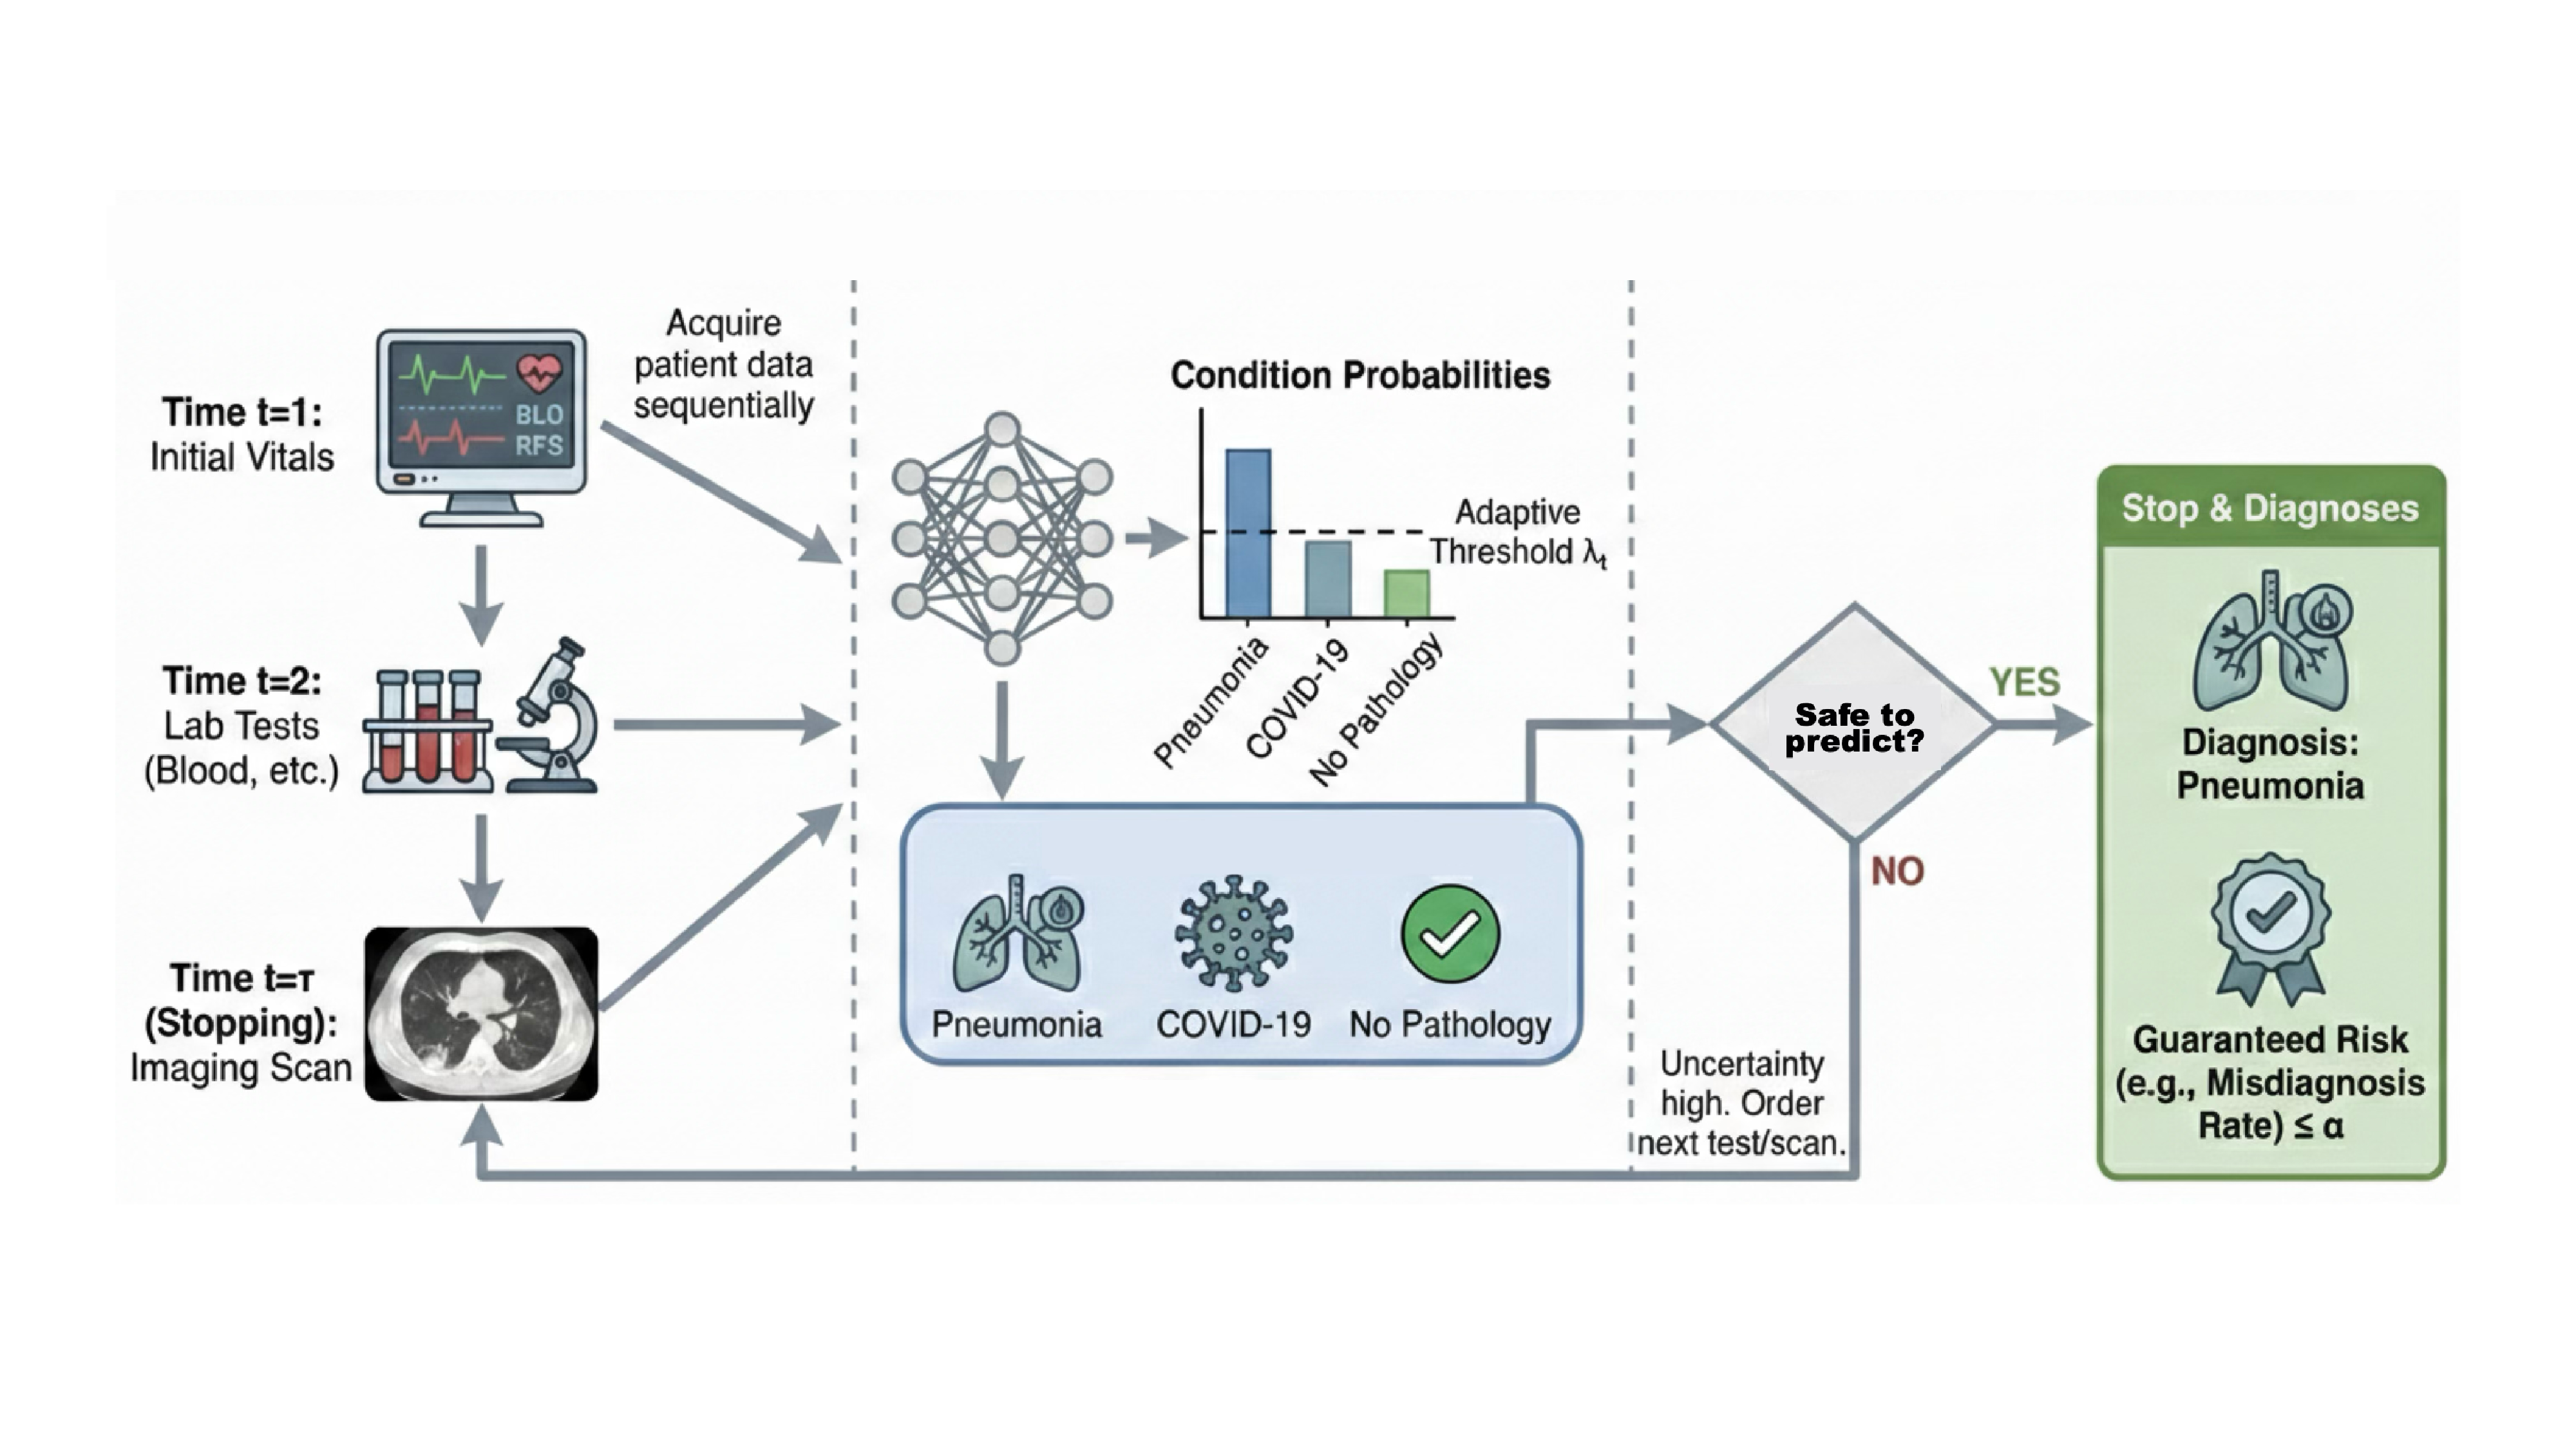
\includegraphics[width=0.8\linewidth]{figures/rcs_figure.pdf}
%     \vspace{-1cm}
%     \caption{\textbf{Risk-controlled stopping (\textsc{rcs}).} Data in clinical pipelines are acquired sequentially and each acquisition is costly. \gls{method} decides when to halt acquisition while guaranteeing that the risk of the resulting decision stays below a user-chosen level.}
%     \label{fig:rcs_figure}
% \end{figure}

The first question has received most of the attention. 
Dynamic feature acquisition methods learn policies that select informative measurements under a cost budget \citep{bakker2020experimental,singhal2023feasibility,covert2023learning,ASMR}. 
The second question is usually settled by a fixed budget, a confidence heuristic, or a learned policy tuned for average accuracy \citep{jafa-2018,bakker2020experimental}. 
None of these approaches offer a guarantee on the risk of the decision made when acquisition halts. 
This is consequential in safety-critical settings like healthcare, where stopping too early could produce unsafe decisions, and stopping too late wastes costs and increases patient burden.

We propose risk-controlled stopping (\textsc{rcs}), a post-hoc, distribution-free procedure for deciding when to stop acquisition so that a user-specified risk, such as misclassification, the false negative rate (\textsc{fnr}), or the false positive rate (\textsc{fpr}), stays below a chosen level. 
Two properties of the controlled risk set \gls{method} apart. 
First, it is an \emph{absolute} risk, measured against the ground-truth label rather than against the prediction the model would have made with all the data. 
Second, it is evaluated \emph{conditional on stopping}: only the samples on which the policy commits to a decision count. 
The second property is important, because a policy that rarely stops but is wrong on almost every sample where it stops can still satisfy a marginal risk bound over the full population.
Whereas a conditional risk bound rules out this behavior. 
%A marginal bound over the whole population is satisfied by a policy that stops rarely and errs on nearly everything it stops on; a conditional bound is not.

The statistical engine behind \gls{method} is the Learn-Then-Test (LTT) framework \citep{angelopoulos2025learn}, which certifies a family of parameterized predictors on a held-out calibration set with finite-sample, distribution-free guarantees. Our key observation is that a stopping rule is a form of selective predictor: it decides both \emph{whether} and \emph{when} to make a prediction, and thus on which partial observation the prediction is made. Treating each rule as a trajectory-level policy lets LTT certify the risk conditional on stopping directly. This guarantee comes from LTT and we do not claim a new bound or proof technique. 
%We are explicit that the certificate is inherited: \cref{thm:conditional_risk} is a corollary of LTT, and we claim no new bound or proof technique. 
Our contribution is the problem formulation, the definition of the risk being controlled, and the procedure needed to control it. 
An absolute risk admits no configuration that is safe by construction, so the set of certifiable rules can be non-monotone or empty. 
\gls{method} therefore calibrates with a step-down procedure rather than fixed-sequence testing, and when no rule can be certified with the available calibration data it defers to full acquisition rather than deploying an uncertified early-stopping policy.

We evaluate \gls{method} on one synthetic and two clinical tasks. The synthetic task, sequential patch acquisition on \textsc{CIFAR-10} \citep{cifar10}, validates the procedure under a controlled acquisition model. 
We draw no clinical conclusions from it. 
The clinical tasks use raw scanner measurements: slice-level abnormality detection from \textsc{fastMRI} knee $k$-space \citep{zbontar2018fastmri}, and PI-RADS-positive classification (radiologist-assigned PI-RADS $\geq 3$) from diffusion-weighted averages in an internal prostate \textsc{mri} cohort. 
Prior work has shown that a well-chosen subset of measurements can support reliable detection at a fixed undersampling factor \citep{singhal2023feasibility,ASMR}; it does not say when, for a given patient, acquisition can stop. \gls{method} answers that question with a certificate. The evaluated MRI checkpoints exhibit class-conditional \textsc{fnr} below the prescribed level; these stage-specific plots are empirical diagnostics, while the statistical certificate pertains to the eventually stopped cohort. The same procedure wraps a learned acquisition policy \citep{jafa-2018} without retraining.

\paragraph{Contributions}
\begin{itemize}[noitemsep]
    \item We propose \emph{risk-controlled stopping}: choosing when to halt sequential acquisition so that an absolute, user-specified risk against the ground-truth label (for example, \textsc{fnr}) is controlled on the samples the policy commits to. To our knowledge, no prior work casts acquisition stopping as a distribution-free, finite-sample risk-control problem.
    \item We show that treating each stopping rule as a trajectory-level selective policy makes this object certifiable by LTT (\cref{thm:conditional_risk} in Section \ref{sec:ltt}), and that the absolute-risk setting forces two design choices absent from relative-risk calibration: Holm's step-down without assuming an ordering of candidate risks, and explicit failure to certify when the certified set is empty, followed by an operational full-acquisition fallback.
    \item We instantiate the framework with class-conditional \textsc{fnr}/\textsc{fpr} and demonstrate certified control on scanner-ordered \textsc{mri} pipelines, on a synthetic \textsc{cifar}-10 benchmark, and as a post-hoc wrapper around a learned reinforcement-learning acquisition policy.
\end{itemize}

\section{Background and Related Work}

\paragraph{Dynamic feature acquisition.}
Acquiring features sequentially at test time has been studied extensively. Early methods select greedily by a utility score \citep{utility2005}, these methods fall into three families distinguished by how they decide to stop. \emph{Fixed budgets and information gain.} EDDI \citep{EDDI} selects the feature with the largest expected information gain and reports curves over budgets. Adapted to dynamic stopping, such methods halt when the largest expected gain falls below a cost threshold $\tau$. The threshold trades information against cost, it bears no direct relation to downstream risk such as an error rate below $5\%$. \emph{Policy-based stopping.} \citet{jafa-2018} and \citet{difa_2023} cast acquisition as a Markov decision process with ``stop'' as an action and maximize a reward $R = \mathbb{I}(y_{\text{pred}} = y_{\text{true}}) - \lambda\,\mbc$. Optimizing an average reward encourages the agent to stop early on hard, expensive instances whenever the cost of more information exceeds the expected loss from an error, which is the opposite of a per-decision safety guarantee. 
% \emph{Heuristic criteria.} Outside learned policies, a common baseline borrows early-exit rules from deep networks and stops when the maximum softmax probability exceeds a threshold such as $0.95$. Deep networks are poorly calibrated and overconfident off-distribution \citep{guo2017}, so a score of $0.95$ does not mean a $95\%$ chance of being right.

\paragraph{Early classification and adaptive halting.}
A parallel literature on time series learns when to halt, and sometimes what to measure next, by optimizing an average objective. \citet{chang2019dynamic} schedule measurements with deep reinforcement learning; EARLIEST \citep{hartvigsen2019adaptive} and the Recurrent Halting Chain \citep{hartvigsen2020recurrent} train halting networks that trade earliness against accuracy. These are strong halting backbones, but the halting point is chosen to be good on average, not certified to control a specified risk on the samples where the model actually stops. 
\gls{method} complements these approaches: as a post-hoc wrapper, it can use the stopping scores of any such policy to certify risk conditional on stopping, as we show for \textsc{jafa} in \cref{sec:experiments_2}.

\paragraph{Conformal prediction and risk control.}
Conformal prediction constructs prediction sets with finite-sample coverage under exchangeability \citep{shafer2008tutorial,angelopoulos2022}, and conformal risk control extends the guarantee from coverage to any bounded risk \citep{angelopoulos2022conformal}. Both certify a \emph{fixed} rule on a \emph{fixed} input. Sequential acquisition violates both premises: the prediction is formed from a partial observation, and the time at which it is formed is chosen from the data. \citet{gauthier2025values} bring conformal ideas to sequential settings, and \citet{jazbec2024fast} calibrate early exits in neural networks to save inference compute. The latter bounds a marginal risk over all inputs and economizes internal computation, we reduce external physical acquisition and bound the risk on the stopped subset.

\paragraph{Closest work.}
\citet{ringel2024early} also calibrate a stopping rule with LTT, for early time-series classification. 
The main difference is the risk being controlled. 
They bound the \emph{accuracy gap}, the rate at which stopping early changes the prediction relative to using the full series.
This measures agreement with the full-data model, rather than correctness. 
For example, a cancer case that the model misses at every step has an accuracy gap of zero and is still a false negative. 
\gls{method} instead bounds the error itself, which changes the calibration problem. 
The accuracy gap is zero at full acquisition, giving their family a configuration that is safe by construction. 
% Their safe rules also form a contiguous sequence that fixed-sequence testing (FST) can test in order. 
An absolute risk has no such guaranteed safe configuration.
% and need not be monotone in the stopping parameter. 
% The set of safe rules can therefore be disconnected or empty.
% This has two consequences. 
% First, \gls{method} may certify nothing and defer to full acquisition when safe early stopping is unattainable, which is the right outcome in a clinical setting. 
% Second, FST can miss safe rules (especially if the safe rule follows an unsafe one) because it halts at the first non-rejection.
% We therefore use Holm's step-down procedure, which can certify safe rules anywhere in the family.

\subsection{The Learn-Then-Test framework}
\label{sec:ltt}
Learn-Then-Test (LTT) \citep{angelopoulos2025learn} calibrates a pre-trained model post hoc. Given a family of predictors $f(\mbx;\lambda)$ indexed by a finite grid $\Lambda = \{\lambda_1,\dots,\lambda_m\}$, a bounded loss $\ell(y,\hat y) \in [0,B]$, a target level $\alpha \in (0,1)$, and a confidence level $\delta \in (0,1)$, LTT selects $\hat\lambda \in \Lambda$ such that
\begin{align}
\label{eq:ltt_guarantee}
    \bbP_{\cD_{\text{cal}}}\left[ \E_{\mbx, y \sim \cP^{\text{data}}}[\ell(y, f(\mbx; \hat{\lambda}))] \le \alpha \right] \ge 1 - \delta.
\end{align}
It does so by treating calibration as multiple hypothesis testing on a held-out set $\cD_{\text{cal}} = \{(\mbx^i, y^i)\}_{i=1}^n$. For each $\lambda$, the null hypothesis $H_{0,\lambda} : R(\lambda) > \alpha$ states that $\lambda$ is unsafe. A concentration inequality for bounded variables (Hoeffding or empirical Bernstein) converts the empirical risk $\widehat{R}(\lambda) = \frac{1}{n}\sum_{i} \ell(y^i, f(\mbx^i; \lambda))$ into a valid p-value $p(\lambda)$. A family-wise error rate procedure at level $\delta$, such as Holm's step-down \citep{holm1979simple}, then rejects a subset of the nulls; the corresponding parameters form the safe set $\widehat{\Lambda}_{\text{safe}}$, and every member of it satisfies \cref{eq:ltt_guarantee}. The user is free to deploy the member that maximizes an application-specific utility $U(\lambda)$.

\section{Problem Setup}
\label{sec:setup}
An input $\mbx = [x_1, \dots, x_d]$ consists of $d$ measurements that are acquired over time. The partial observation after $t$ steps is $\mbx_t = \mbx \circ \mbs_t$, where $\mbs_t \in \{0,1\}^d$ is a mask marking the components acquired so far and $\circ$ is element-wise multiplication. The acquisition policy that produces $\mbs_t$ may be fixed in advance, random, or adaptive (a function of $\mbx_{t-1}$); in every case the observations are nested. 
Full trajectories $(\mbx^i, y^i)$ are drawn i.i.d.\ from an unknown distribution $\cP^{\text{data}}$, and we hold out a calibration set $\cD_{\text{cal}} = \{(\mbx^i, y^i)\}_{i=1}^{n}$. 
A pre-trained predictor $p_\theta$ returns a prediction $\hat{y}(\mbx_t)$ from any partial observation. We seek a data-dependent \emph{stopping time} $\tau(\mbx) \in \{1, \dots, d\} \cup \{\infty\}$ at which acquisition halts and the system commits to $\hat{y}(\mbx_\tau)$; $\tau(\mbx) = \infty$ means the policy defers to full acquisition.

\paragraph{Why bounding the marginal risk is not sufficient. }
It is tempting to bound the marginal risk of the stopped output, $\bbP(E_\tau)$, where $E_\tau$ is the event that the policy stopped and made an error.
Let $S = \{\tau(\mbx) < \infty\}$ be the event that the policy stops and commits to a prediction. 
Since, deferred samples do not count as errors from stopping, we have $E_\tau \subseteq S$ and
\begin{align}
\label{eq:marg_decomp}
    \bbP(E_\tau) = \bbP(E_\tau \mid S)\,\bbP(S).
\end{align}
A marginal bound $\bbP(E_\tau) \le \alpha$ therefore says nothing about the error among committed decisions, $\bbP(E_\tau \mid S)$, unless $\bbP(S)$ is close to one. 
A policy that commits on $1\%$ of samples and is wrong on every one of them satisfies $\bbP(E_\tau) = 0.01 \le \alpha$ while being useless. 
What a clinician needs is the reliability of the decisions that are actually made. \gls{method} therefore controls the risk \emph{conditional on stopping}.

\section{Risk-Controlled Safe Stopping via Policy-Level Certification}
\label{sec:rcs}

We first define the risk conditional on stopping and show how to test each candidate policy using the calibration samples on which it stops. 
We then combine these tests to certify a set of policies and select one based on a user-chosen utility, defaulting to full acquisition if none can be certified. 
Finally, we extend the procedure to class-conditional false negative and false positive rates and describe the stopping rules used in our experiments.

% \gls{method} treats each candidate stopping rule as a complete trajectory-level policy, measures the loss it incurs on the calibration trajectories it stops on, and uses the LTT machinery of \cref{sec:ltt} to certify which rules control the conditional risk.

\subsection{Conditional risk of a stopping policy}
Consider a family of stopping rules $\cD_\textsc{stop}(\mbx_t; \lambda) \in \{0, 1\}$ indexed by a finite grid $\lambda \in \Lambda = \{\lambda_1, \dots, \lambda_m\}$. Each rule induces a stopping time, the first step at which it fires,
\begin{align}
\label{eq:stopping_time}
    \tau_\lambda(\mbx) = \inf\{t \in \{1, \dots, d \} \mid \cD_\textsc{stop}(\mbx_t; \lambda) = 1\},
\end{align}
with $\tau_\lambda(\mbx) = \infty$ if the rule never fires, in which case the policy defers to full acquisition. When it fires at $t \le d$, the system commits to $\hat{y}(\mbx_t)$. For a bounded loss $\ell(y, \hat{y}) \in [0, B]$, the quantity we control is the expected loss given that the policy stops,
\begin{align}
\label{eq:cond_risk_def}
    R_{\text{cond}}(\lambda) = \E_{\mbx, y \sim \cP^{\text{data}}}\left[\ell\left(y, \hat{y}(\mbx_{\tau_\lambda(\mbx)})\right) \;\middle|\; \tau_\lambda(\mbx) < \infty \right].
\end{align}
Our goal is to select a $\hat{\lambda} \in \Lambda$ with $R_{\text{cond}}(\hat\lambda) \le \alpha$ with probability at least $1-\delta$ over the draw of $\cD_{\text{cal}}$. 
Changing $\lambda$ changes not only \emph{which} samples the policy stops on, but also changes \emph{when} it stops. 
It therefore also changes the partial observation each prediction is made. 
The map $\lambda \mapsto R_{\text{cond}}(\lambda)$ can therefore jump and need not be monotone.

\paragraph{Testing each policy on the samples it stops.}
For each $\lambda$, let $\cS(\lambda) = \{ i \le n \mid \tau_\lambda(\mbx_i) < \infty \}$ be the indices of the calibration samples where the policy stops, and let $n(\lambda) = |\cS(\lambda)|$. 
The empirical conditional risk is the mean loss over this subset,
\begin{align}
    \widehat{R}_{\text{cond}}(\lambda) = \frac{1}{n(\lambda)} \sum_{i \in \cS(\lambda)} \ell\left(y^i, \hat{y}(\mbx^i_{ \tau_\lambda(\mbx^i)})\right),
\end{align}
and we test $H_{0,\lambda} : R_{\text{cond}}(\lambda) > \alpha$.
The set $\cS(\lambda)$ is selected by the very rule under test. 
Because the calibration trajectories are i.i.d.\ and membership in $\cS(\lambda)$ depends only on the trajectory itself, the stopped samples are conditional on $n(\lambda)$ draws from the distribution conditioned on stopping. 
Hoeffding's inequality then yields a p-value that is valid conditional on $n(\lambda)$,
\begin{align}
\label{eq:hoeffding_pvalue}
    p(\lambda) =
    \begin{cases}
        1, & \text{if } n(\lambda) = 0 \text{ or } \widehat{R}_{\text{cond}}(\lambda) \ge \alpha, \\[2pt]
        \exp\!\left(-2 n(\lambda)\big(\alpha - \widehat{R}_{\text{cond}}(\lambda)\big)^2 / B^2\right), & \text{otherwise}.
    \end{cases}
\end{align}
This conditional validity also makes the p-value valid over the random draw of the calibration set. 
%and validity conditional on $n(\lambda)$ implies validity marginally over the calibration set.

\paragraph{Multiplicity correction and selection.}
Testing $m$ hypotheses at once calls for family-wise error control. We apply Holm's step-down procedure \citep{holm1979simple}: sort the p-values $p_{(1)} \le \cdots \le p_{(m)}$, reject $H_{(j)}$ as long as $p_{(j)} \le \delta/(m-j+1)$, and stop at the first failure. The rejected hypotheses form the safe set $\widehat{\Lambda}_{\text{safe}}$, and every $\lambda$ in it controls the conditional risk. We deploy the safe rule that maximizes a user-chosen utility $U(\lambda)$, typically the fraction of samples stopped or the negative mean stopping time. If $\widehat{\Lambda}_{\text{safe}}$ is empty, \gls{method} reports that no candidate could be certified at the chosen confidence level using the available calibration data, and every sample proceeds to full acquisition. This does not establish that no safe candidate exists or certify the risk of the full-acquisition predictor.

\begin{corollary}[Conditional risk control; corollary of LTT]
    \label{thm:conditional_risk}
    Let $\cD_{\text{cal}}$ consist of $n$ i.i.d.\ sample trajectories and let $\hat{\lambda}$ be selected by the procedure above. Then, provided $\widehat{\Lambda}_{\text{safe}} \neq \emptyset$,
    \begin{align}
        \bbP_{\cD_{\text{cal}}}\left[ \E_{\mbx, y} \left[ \ell\left(y, \hat{y}(\mbx_{\tau_{\hat\lambda}(\mbx)})\right) \;\middle|\; \tau_{\hat{\lambda}}(\mbx) < \infty \right] \leq \alpha \right] \geq 1 - \delta.
    \end{align}
\end{corollary}
The result is a direct application of LTT \citep{angelopoulos2025learn}: each $\lambda$ is a selective predictor on trajectories, and LTT already certifies a selective risk over a data-dependent selected subset. 
The argument requires a policy family and selection events fixed independently of the risk-calibration labels, and independent calibration trajectories drawn from the same induced distribution as deployment trajectories. The guarantee concerns the eventually stopped cohort $\{\tau_{\hat\lambda}<\infty\}$; it does not assert simultaneous risk control for the cumulative cohorts $\{\tau_{\hat\lambda}\le t\}$ at every checkpoint.
%The argument uses nothing about the selection event beyond its being fixed before calibration, so it applies verbatim to any pre-specified event. 
Pseudocode is given in \cref{eq:alg_ltt} in the appendix.

\subsection{Class-conditional FNR and FPR}
\label{sec:fnr_fpr}
\Cref{eq:cond_risk_def} covers mis-classification directly. Clinical practice asks instead for class-conditional rates: the false negative rate among truly positive cases and the false positive rate among truly negative ones, rather than a pooled or prevalence-weighted error. For a task with labels $y \in \{0,1\}^K$ (binary when $K=1$) we certify, for each label $k$,
\begin{align}
    \mathrm{FNR}_k(\lambda) = \bbP\!\left(\hat{y}_k(\mbx_{\tau_\lambda}) = 0 \;\middle|\; y_k = 1,\ \tau_\lambda(\mbx) < \infty\right) \le \alpha_k,
\end{align}
and $\mathrm{FPR}_k$ symmetrically. This is the conditional risk of \cref{eq:cond_risk_def} under the refined selection event $\{y_k = 1,\ \tau_\lambda < \infty\}$: the effective calibration set is the stopped positives $\cS^+_k(\lambda) = \{ i : \tau_\lambda(\mbx^i) < \infty,\ y^{i}_k=1 \}$ and the loss is $\mathbf{1}\{\hat y^i_{k}=0\}$. Because the loss is binary we replace Hoeffding with the exact binomial tail, which is tighter, and we combine labels by $p(\lambda) = \max_k p_k(\lambda)$, which is valid under arbitrary dependence between labels and accommodates label-specific targets $\alpha_k$. The policy family, the stopping rule, and the Holm correction are unchanged. Class-conditional certification requires sufficient stopped positive (or negative) calibration examples; a policy with none cannot be certified for that class.

\paragraph{Policy families.}
\gls{method} places no restriction on the form of the stopping rule beyond the family being fixed before calibration. We use three. A \emph{confidence threshold} on the softmax score (\textsc{cifar}-10); the \emph{\textsc{jafa} Q-margin}, the gap between the Q-value of ``stop'' and that of the best acquisition action (\cref{sec:experiments_2}); and \emph{ambiguity bands} for the \textsc{mri} tasks, where $\lambda \in [0,1]$ scales a per-label uncertainty band from never stopping ($\lambda = 0$) to an aggressive data-driven band ($\lambda = 1$), and the rule fires once every label's score has left its band (\cref{app:ambiguity_bands}).

\section{Experiments}
We evaluate the proposed stopping-calibration procedure in two complementary settings. 
In \cref{sec:experiments_1}, we consider fixed acquisition trajectories across vision and medical-imaging benchmarks to assess whether the method controls the target risk while reducing the number of measurements acquired. 
In Section \ref{sec:experiments_2}, we extend the evaluation to learned adaptive acquisition policies by applying our method as a post-hoc wrapper around JAFA (Shim et al., 2018), a reinforcement-learning-based acquisition model. 
We assess whether the wrapped system controls the target risk while retaining the efficiency of the underlying adaptive policy.
%We evaluate \gls{method} in two complementary settings. In section-\ref{sec:experiments_1}, we study its behavior on a diverse set of sequential acquisition problems under fixed acquisition trajectories. The goal of this section is to assess whether the proposed method achieves the desired risk control while retaining practical stopping efficiency across vision and medical-imaging benchmarks. In section \ref{sec:experiments_2}, we demonstrate that our method is complementary to learned adaptive acquisition policies by wrapping them around a reinforcement-learning-based acquisition backbone, JAFA \citep{jafa-2018}, and evaluating whether the resulting wrapped system preserves the desired risk guarantees while retaining the efficiency of the underlying adaptive policy.

\begin{figure}[h]
    \centering
    \begin{minipage}[t]{0.4\linewidth}
        \centering
        
\includegraphics[width=\linewidth]{figures/cifar_mask_example.png}
    \end{minipage}
    \begin{minipage}[t]{0.4\linewidth}
        \centering
        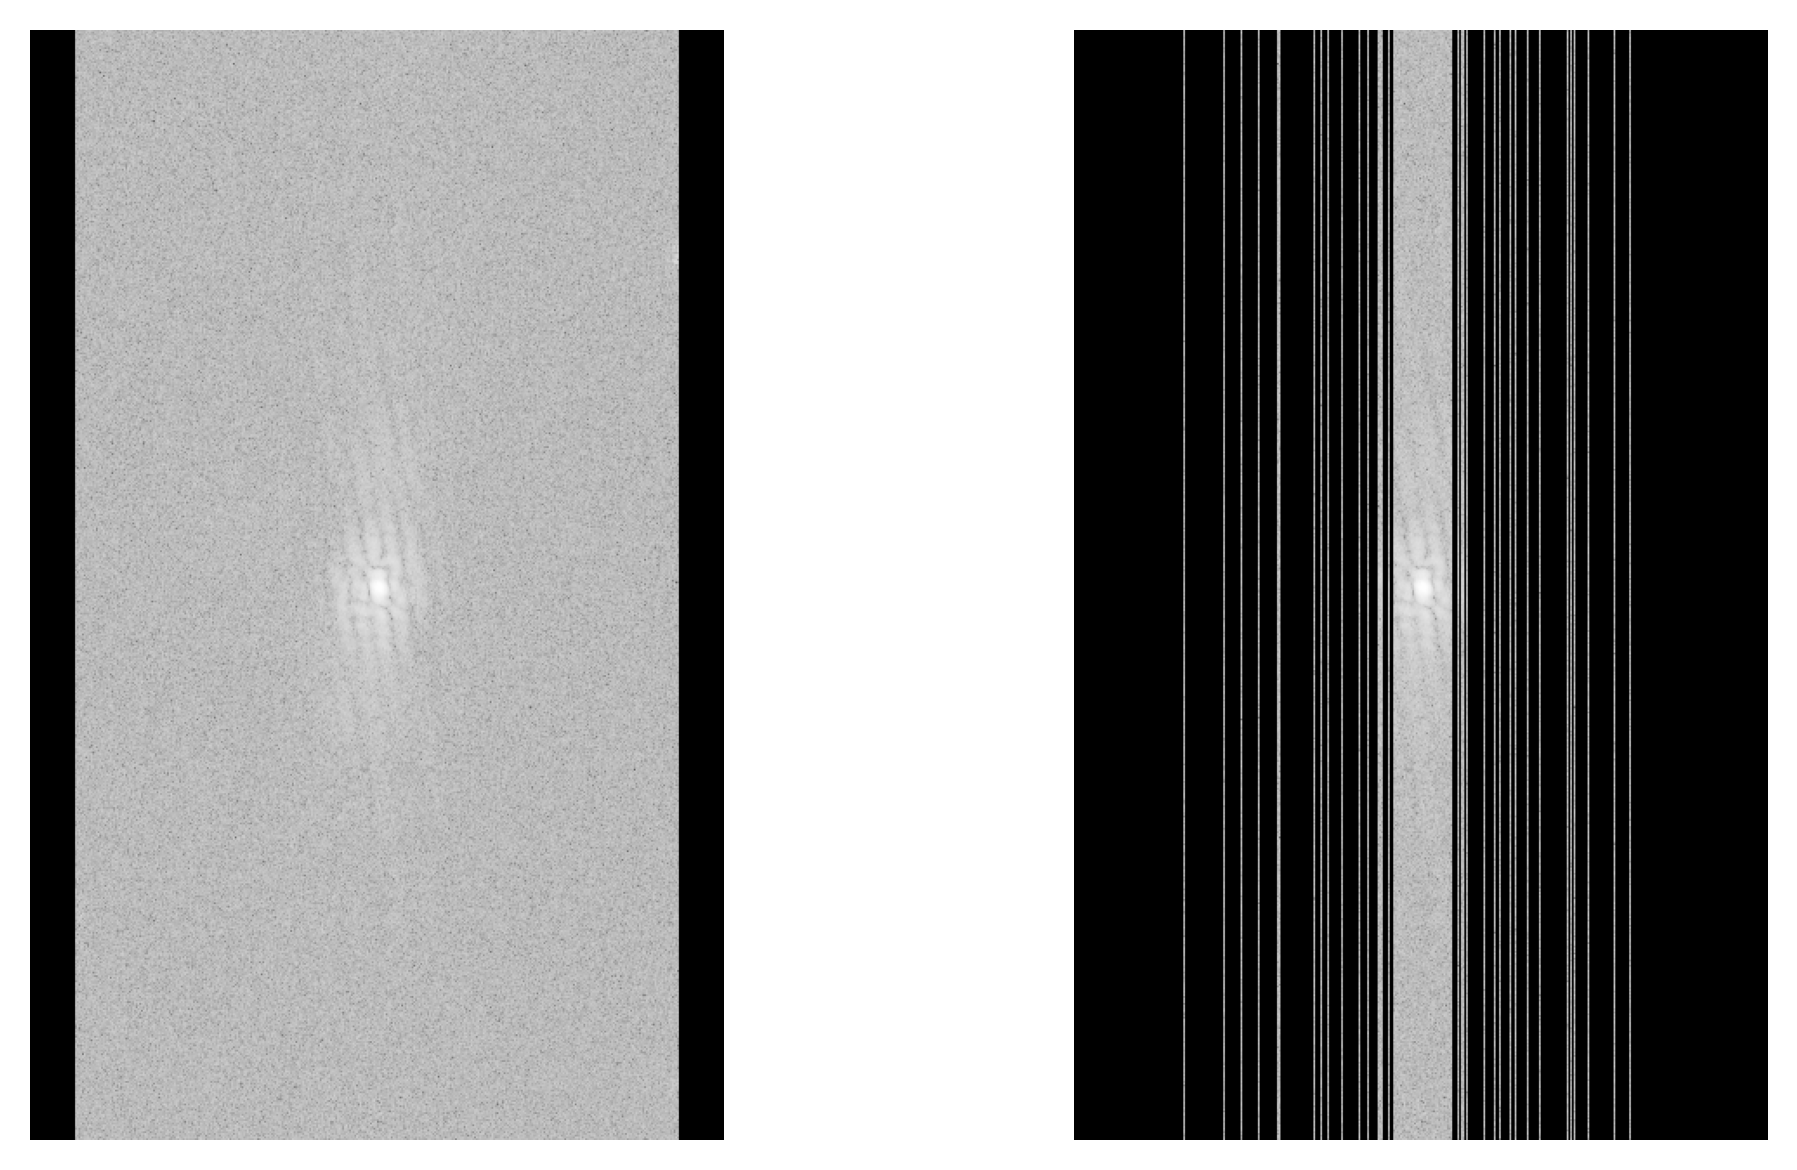
\includegraphics[width=\linewidth]{figures/kspace_mask_example.png}
    \end{minipage}
    \caption{\textbf{Examples of sequential data acquisition in synthetic and \textsc{mr} settings.} 
    \textbf{Left:} in the synthetic regime, the fully observed image $\mbx$ is partitioned into non-overlapping patches, each treated as a feature to be acquired sequentially; the right panel within that image shows the partially observed image $\mbx_t$ after acquisition of $t$ patches. 
    \textbf{Right:} in the \textsc{mr} setting, the left panel shows a fully sampled \textit{k}-space, and the right panel shows the same \textit{k}-space at an intermediate acquisition step.}
    \label{fig:acquisition_examples}
\end{figure}



\subsection{Datasets}
We use the following datasets that span both synthetic and real-world acquisition settings:
\begin{enumerate}[noitemsep]
    \item {\bf CIFAR-10} is a widely used benchmark dataset for image classification, consisting of $60,000$ images of size $32 \times 32 \times 3$ pixels, divided into $10$ object classes, with each class equally represented \citep{cifar10}. 
    
    \item {\bf FastMRI Knee} dataset  \citep{zbontar2018fastmri} provides open-source fully-sampled \textit{k-space} data associated with the knee MR scans. It consists of a total of $41679$ 2D slices, refer to \cref{tab:fastmri_class_stats} in appendices, for the full data statistics. The diagnostic task involves detecting two musculoskeletal abnormalities: {ACL tear} and {meniscus tear}, a standard set of pathologies diagnosed in clinical tasks \citep{singhal2023feasibility,ASMR}. Since these labels are not mutually exclusive, we treat this as a multi-label classification problem.
    
    \item {\bf Clinical Prostate MRI (Internal dataset)} is a large de-identified prostate MRI cohort from an urban health system. The task is binary PI-RADS-positive classification, defined as radiologist-assigned PI-RADS $\geq$ 3, an MRI-based marker of suspicion for clinically significant prostate cancer~\citep{turkbey2019pirads}. Each scan contains an axial T2-weighted volume and diffusion-weighted imaging (DWI). Split statistics and class prevalence are reported in appendices \cref{tab:prostate_dataset_stats}

\end{enumerate}

\subsection{Score Functions}
Our calibration procedures operate on score functions evaluated on a held-out calibration set. We train deep neural network classifiers to obtain these score functions. For CIFAR-10, we train a ResNet-18 \citep{he2016deep} on randomly masked images, to maximize the log likelihood of the associated labels. For the FastMRI Knee and Prostate datasets, we follow the recipe of \citet{singhal2023feasibility} to train classifiers on undersampled $k$-space data.

\begin{figure*}[t]
\centering
    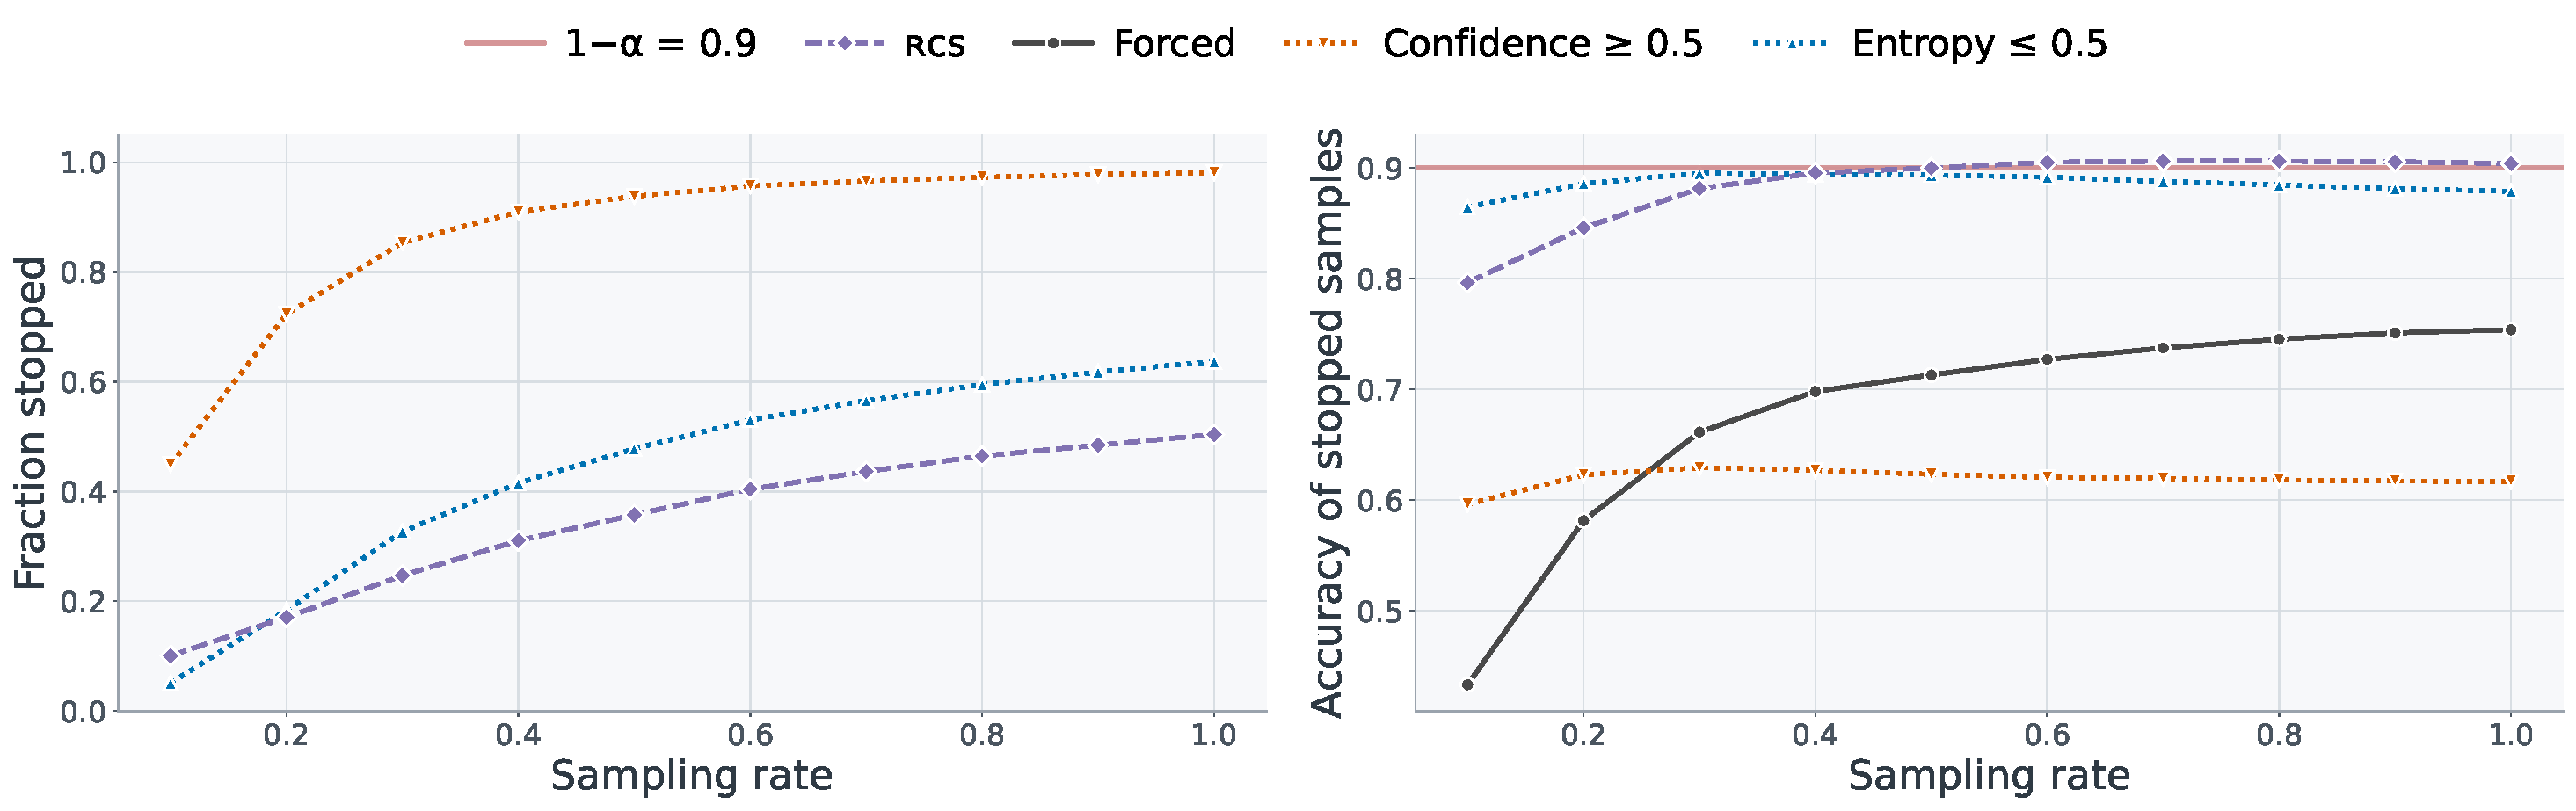
\includegraphics[width=\linewidth]{figures/compare_panel_max_score.pdf}
    \caption{\textbf{Control of misclassification rates on \textsc{CIFAR-10}.} \textbf{Left:} The cumulative fraction of samples halted at each sampling stage. \textbf{Right:} Predictive accuracy of stopped samples as a function of the number of acquired patches. We observe that \gls{method} successfully maintains the misclassification rate below the specified risk level ($\alpha = 0.1$), whereas heuristic baselines consistently violate the safety threshold.}
    \label{fig:cifar-10}
\end{figure*}

\subsection{Evaluation on Sequential Acquisition Tasks}
\label{sec:experiments_1}
We first evaluate the proposed methods on three datasets: CIFAR-10 for object classification with sequential acquisition simulated through patch masking; FastMRI Knee for slice-level musculoskeletal abnormality detection from sequentially acquired $k$-space lines; and Clinical Prostate MRI for PI-RADS-positive classification from sequentially acquired DWI averages, with axial T2 held fixed. 
Examples of the CIFAR-10 and FastMRI Knee acquisition processes appear in \cref{fig:acquisition_examples}. 
For each dataset, we plot the cumulative fraction of examples stopped and the performance on those examples as functions of the acquisition rate. 
We report stopped-sample accuracy for CIFAR-10. 
For FastMRI Knee, we report the class-conditional false negative rate (\textsc{fnr}) among stopped positives for each controlled pathology (ACL tear and meniscus tear) alongside balanced accuracy. 
For Clinical Prostate MRI, we report \textsc{fnr} among stopped PI-RADS-positive exams ($\mathrm{PI\textrm{-}RADS}\geq3$), also alongside balanced accuracy.



% We first evaluate the proposed methods on three datasets, a synthetic task and two clinical tasks.
% \begin{itemize}[noitemsep]
%     \item \textbf{CIFAR-10}: object classification with simulated sequential acquisition via patch masking, see \cref{fig:acquisition_examples}

%     \item \textbf{FastMRI Knee}: slice-level musculoskeletal abnormality detection from sequentially acquired $k$-space lines, see \cref{fig:acquisition_examples}
%     \item \textbf{Clinical Prostate MRI}: PI-RADS-positive classification from sequentially acquired DWI averages, with axial T2 held fixed
% \end{itemize}


\begin{figure*}[h!]
  %\vskip 0.2in
  \begin{center}
    \centerline{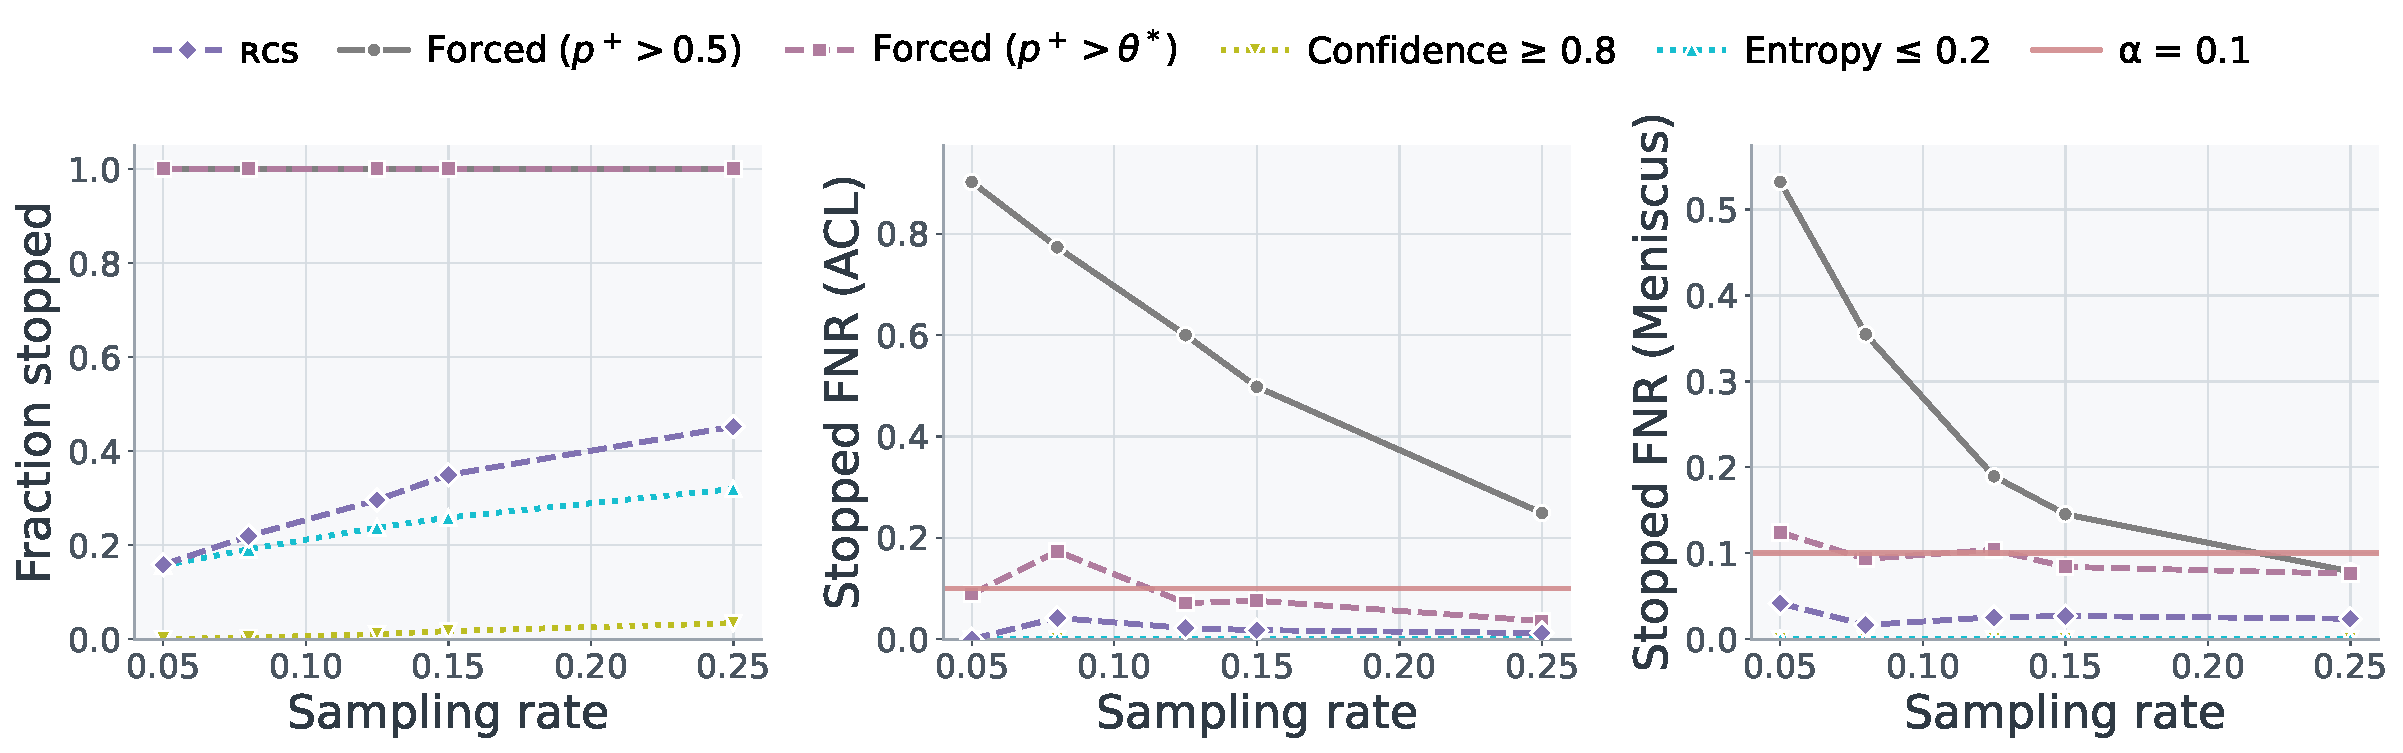
\includegraphics[width=\linewidth]{figures/compare_panel_knee_slice_fnr_conditional_1x3.pdf}}
    \caption{
      \textbf{Class-conditional false negative control on \textsc{FastMRI} knee (\textsc{ACL} tear and meniscus tear).}
      We decide whether to halt slice-level \textit{k}-space collection at sampling rates
      $\cT = \{5\%, 8\%, 12.5\%, 15\%, 25\%\}$.
      The panel reports stopped fraction together with class-conditional \textsc{fnr} among stopped
      positives for \textsc{ACL} tears and meniscus tears
      We observe that \gls{method} controls each pathology-specific \textsc{fnr} at the
      user-specified level ($\alpha = 0.1$) across acquisition rates, including at low
      undersampling such as $5\%$, while heuristic baselines violate the threshold.
      }
      \label{fig:knee-slice-results}
  \end{center}
\end{figure*}


\begin{figure*}[h!]
  %\vskip 0.2in
  \begin{center}
    \centerline{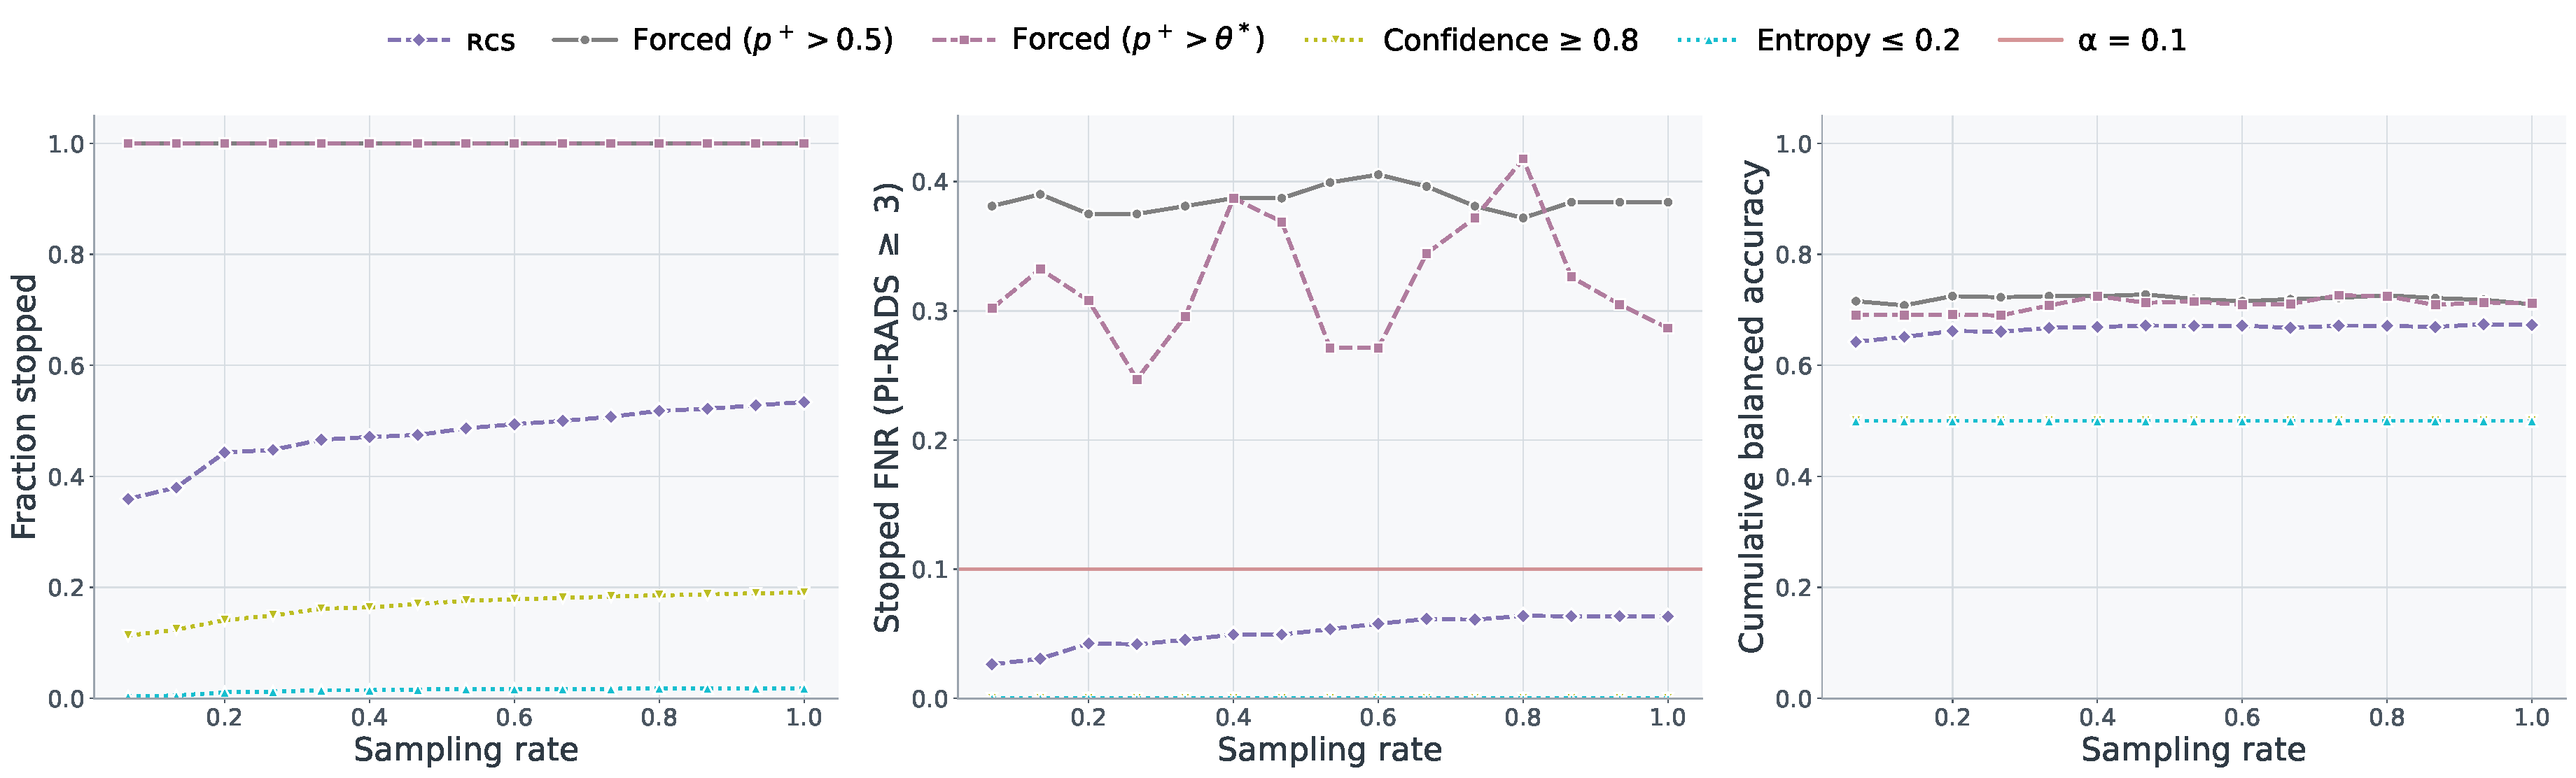
\includegraphics[width=\linewidth]{figures/compare_panel_prostate_pirads_fnr_asym_conditional.pdf}}
    \caption{
      \textbf{Controlling false negative rate (\textsc{fnr}) among stopped exams on Prostate PI-RADS classification.}
      We decide whether to halt acquiring diffusion averages for DWI sequences along the scanner-ordered
      reconstruction checkpoints.
      \textbf{Left:} fraction of exams stopped by \gls{method} and heuristic criteria.
      \textbf{Center/Right:} \textsc{fnr} and balanced accuracy on the stopped cohort, where the controlled
      risk is the false-negative rate among PI-RADS-positive exams ($\mathrm{PI\textrm{-}RADS}\!\geq\!3$)
      that have already been halted.
      We observe that \gls{method} maintains this stopped-sample \textsc{fnr} at the user-specified level
      ($\alpha = 0.1$) across acquisition stages, whereas baseline strategies violate the safety threshold.}
      \label{fig:prostate-results}
  \end{center}
\end{figure*}

% \paragraph{Evaluations.} For each dataset, we plot:
% \begin{enumerate}
%     \item \textbf{Stopped fraction v/s acquisition rate:} the cumulative fraction of examples for which acquisition has been halted by each acquisition time
%     \item \textbf{Stopped-sample performance v/s acquisition rate:} the performance of the subset of stopped examples, measured by the task-relevant risk criteria.
% \end{enumerate}
% For CIFAR-10, we report stopped-sample accuracy. For FastMRI knee, we report \emph{class-conditional} false negative rate (\textsc{fnr}) among stopped positives for each controlled pathology (ACL tear and meniscus tear), together with balanced accuracy. For Clinical Prostate MRI, we report \textsc{fnr} among stopped PI-RADS-positive exams ($\mathrm{PI\textrm{-}RADS}\!\geq\!3$), again alongside balanced accuracy.

\paragraph{Acquisition setup.} For CIFAR-10, we simulate sequential acquisition by partitioning each image into $4 \times 4$ non-overlapping patches and acquiring these patches progressively over time. For the knee MRI dataset, we simulate sequential acquisition directly in the raw $k$-space domain, where each acquisition step reveals additional frequency-domain lines. This matches the underlying measurement process and allows us to evaluate stopping decisions in a clinically realistic acquisition regime.
For Clinical Prostate MRI, sequential acquisition follows the scanner order of the DWI sequence. The axial T2-weighted volume is acquired before the DWI sequence and is fixed across all states. The full DWI protocol contains 48 acquired DWI measurements: 12 at $b=50\,\mathrm{s/mm^2}$, with 4 repeats per diffusion direction, and 36 at $b=1000\,\mathrm{s/mm^2}$, with 12 repeats per direction. Stopping policies are evaluated at 15 scanner-ordered reconstruction checkpoints. At each checkpoint, ADC and computed high-$b$ ($b=1500\,\mathrm{s/mm^2}$) DWI volumes are reconstructed only from the measurements acquired so far, consistent with PI-RADS v2.1 guidance~\citep{turkbey2019pirads}. Later checkpoints therefore contain progressively higher-SNR diffusion information. A fixed 3D T2+DWI fusion classifier produces a PI-RADS-positive score at each checkpoint~\citep{johnson2025prostate}. Appendix Figure~\ref{fig:prostate_dwi_acquisition_states} visualizes DWI-derived reconstructions across the acquisition trajectory.

\paragraph{Baselines.} As baselines, we compare \gls{method} to three potentially ``unsafe" strategies. 
First, \textbf{Forced with Static Decision Thresholds} where the model is forced to make a prediction for every sample across all sampling rates. 
The score threshold used to generate the prediction is a static scalar (we use $p^+ > 0.5$).
This is referred to as ``Forced ($p^+ > 0.5$)" in  Figures \ref{fig:knee-slice-results} and \ref{fig:prostate-results}.
Second, \textbf{Forced with Calibrated Decision Thresholds} where the model is forced to make a prediction for every sample across all sampling rates. 
The score threshold used to make a prediction at each sampling rate is calibrated to maximize some metric of interest (we use balanced accuracy). 
This is referred to as ``Forced ($p^+ > \theta^*$)" in Figures \ref{fig:knee-slice-results} and \ref{fig:prostate-results}.
Third, \textbf{Heuristic Stopping Thresholds} determine dynamic stopping times based on some heuristic threshold on the scores. 
We use Confidence and Entropy of the predictions.


\paragraph{Results.} 
For our synthetic CIFAR-10 experiment, we use the misclassification rate as the risk ($R(y, C_{\alpha}(\mbx_t, t)) = \mathbf{I}(y \not\in C_\alpha(\mbx_t, t))$), and control it at the rate of $10\%$ ($\alpha=0.1$), implying a target coverage/accuracy of $90\%$. 
For both datasets, we report performance as a function of the percentage of features acquired (a.k.a., the acquisition rate) and at every acquisition rate, we track the cumulative percentage of stopped samples. 
This is a direct indicator of our proposed guarantee: for all stopped samples, we maintain an accuracy level corresponding to the input miss-coverage rate ($\alpha$). We compare the performance of \gls{method} against the Fixed Sampling Rate Stopping or ``Forced", Confidence-based Thresholding, and Entropy-based Thresholding. See Figure~\ref{fig:cifar-10} for results on \textsc{cifar-10} dataset. Thresholds for the Entropy and Confidence baselines are set to $0.5$.

In our clinical diagnosis tasks, the risk of interest is false-negative error among sample that have been stopped.
For FastMRI knee, this is instantiated as a \emph{class-conditional} multi-label guarantee: we control pathology-specific \textsc{fnr} for ACL tear and meniscus tear separately, and we report the corresponding per-pathology curves in \cref{fig:knee-slice-results}.
For Prostate PI-RADS, the task is binary, so the same stopped-sample \textsc{fnr} reduces to control among PI-RADS-positive exams in \cref{fig:prostate-results}.

We instantiate $\cD_\textsc{stop}(\mbx_t; \lambda)$ using \emph{ambiguity-band stopping rules}. For each acquisition time $t$ and task $k$, we define an uncertainty interval $[\ell_{t,k}(\lambda), u_{t,k}(\lambda)]$. The parameter $\lambda \in [0, 1]$ scales the band's width, interpolating from maximal ambiguity (highly conservative) to a narrow, data-driven baseline (aggressive). The policy halts acquisition at the first step where predictive scores for \emph{all} controlled tasks exit their respective bands, assigning terminal predictions based on the side of the exit. While we detail this specific band construction in Appendix \ref{app:ambiguity_bands}, our \gls{method} guarantees remain valid for any arbitrary stopping rule parameterized by $\lambda$. 

In \cref{fig:knee-slice-results,fig:prostate-results} we observe that \gls{method} shows efficient stopping behavior while always adhering to the risk constraint. Furthermore, across both sets of experiments, we observe that even though the baseline method ``Forced ($p^+ > \theta^*$)" is calibrated to maximize the balanced accuracy, \gls{method} shows comparable performance while never violating the risk threshold.

\paragraph{Sensitivity to the risk level $\alpha$.}
Beyond fixed operating points, we study how stopping behavior changes as the user varies the allowed risk $\alpha$.
For each $\alpha$ on a grid, we re-select the certified threshold $\widehat{\lambda}(\alpha)$ on the same calibration scores and evaluate the resulting policy on the held-out test set.
\cref{fig:alpha-sweep} summarizes these sweeps for FastMRI knee and Prostate PI-RADS.
The top panels show the cumulative stopped fraction versus acquisition rate, with one curve per $\alpha$: larger $\alpha$ (more permissive risk) yields earlier and more frequent stopping.
The bottom panel reports the expected acquisition rate at stopping, $\mathbb{E}[r_{\mathrm{stop}}]$, as a function of $\alpha$, quantifying the efficiency--risk tradeoff induced by calibration.
As expected, $\mathbb{E}[r_{\mathrm{stop}}]$ decreases monotonically as $\alpha$ increases, while the fixed-$\alpha$ panels above confirm that the corresponding stopped cohorts remain consistent with the requested risk level.

\begin{figure*}[t]
  \vskip 0.2in
  \begin{center}
    \centerline{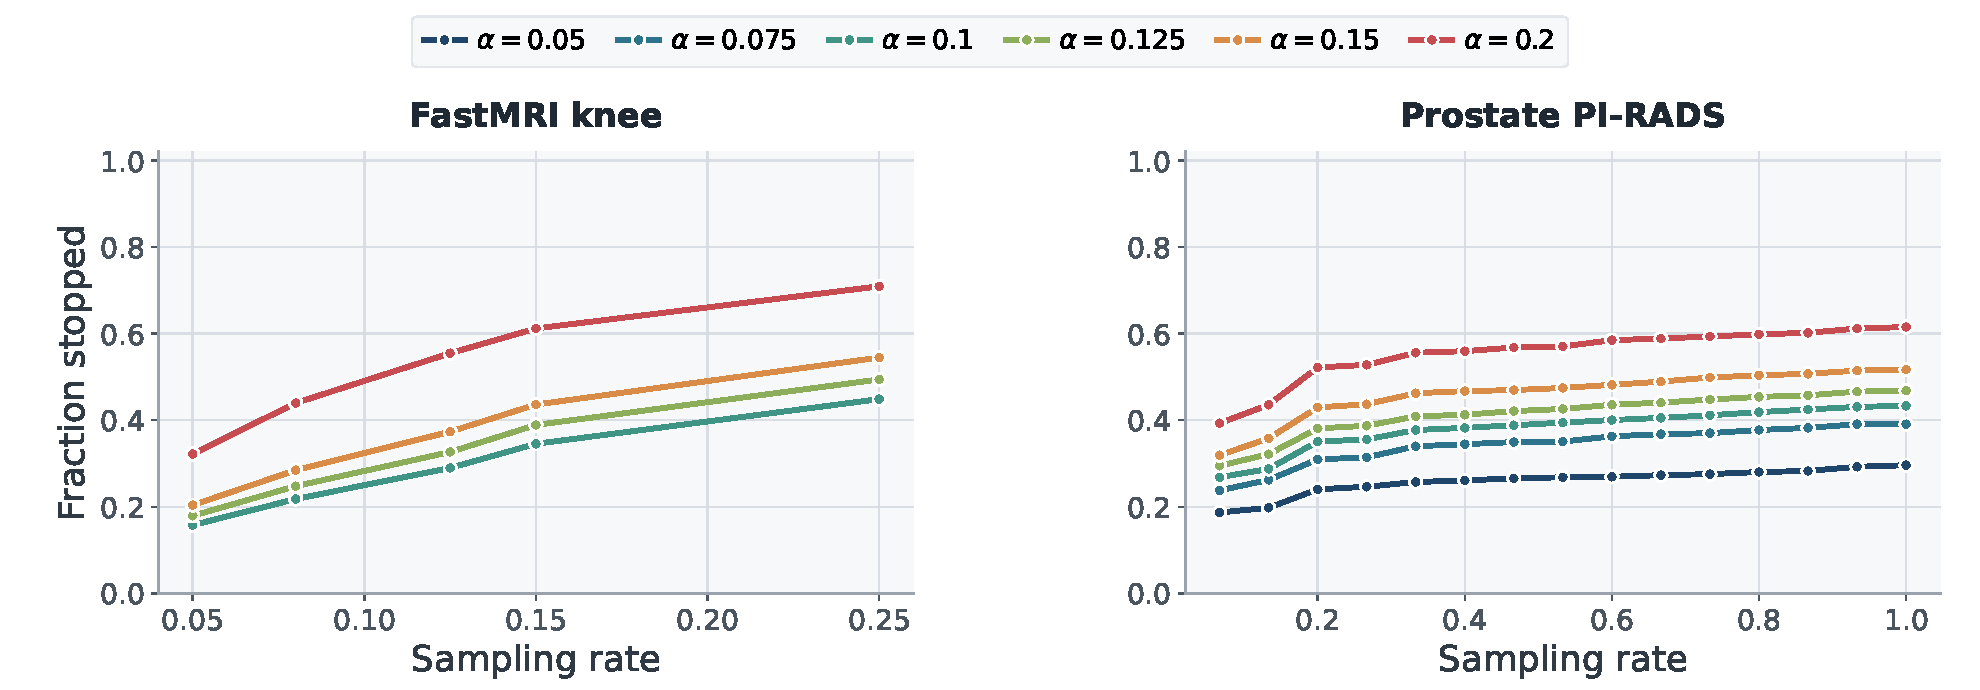
\includegraphics[width=\linewidth]{figures/alpha_stopping_mri_panel_top.pdf}}

    \vspace{0.1in}
    \centerline{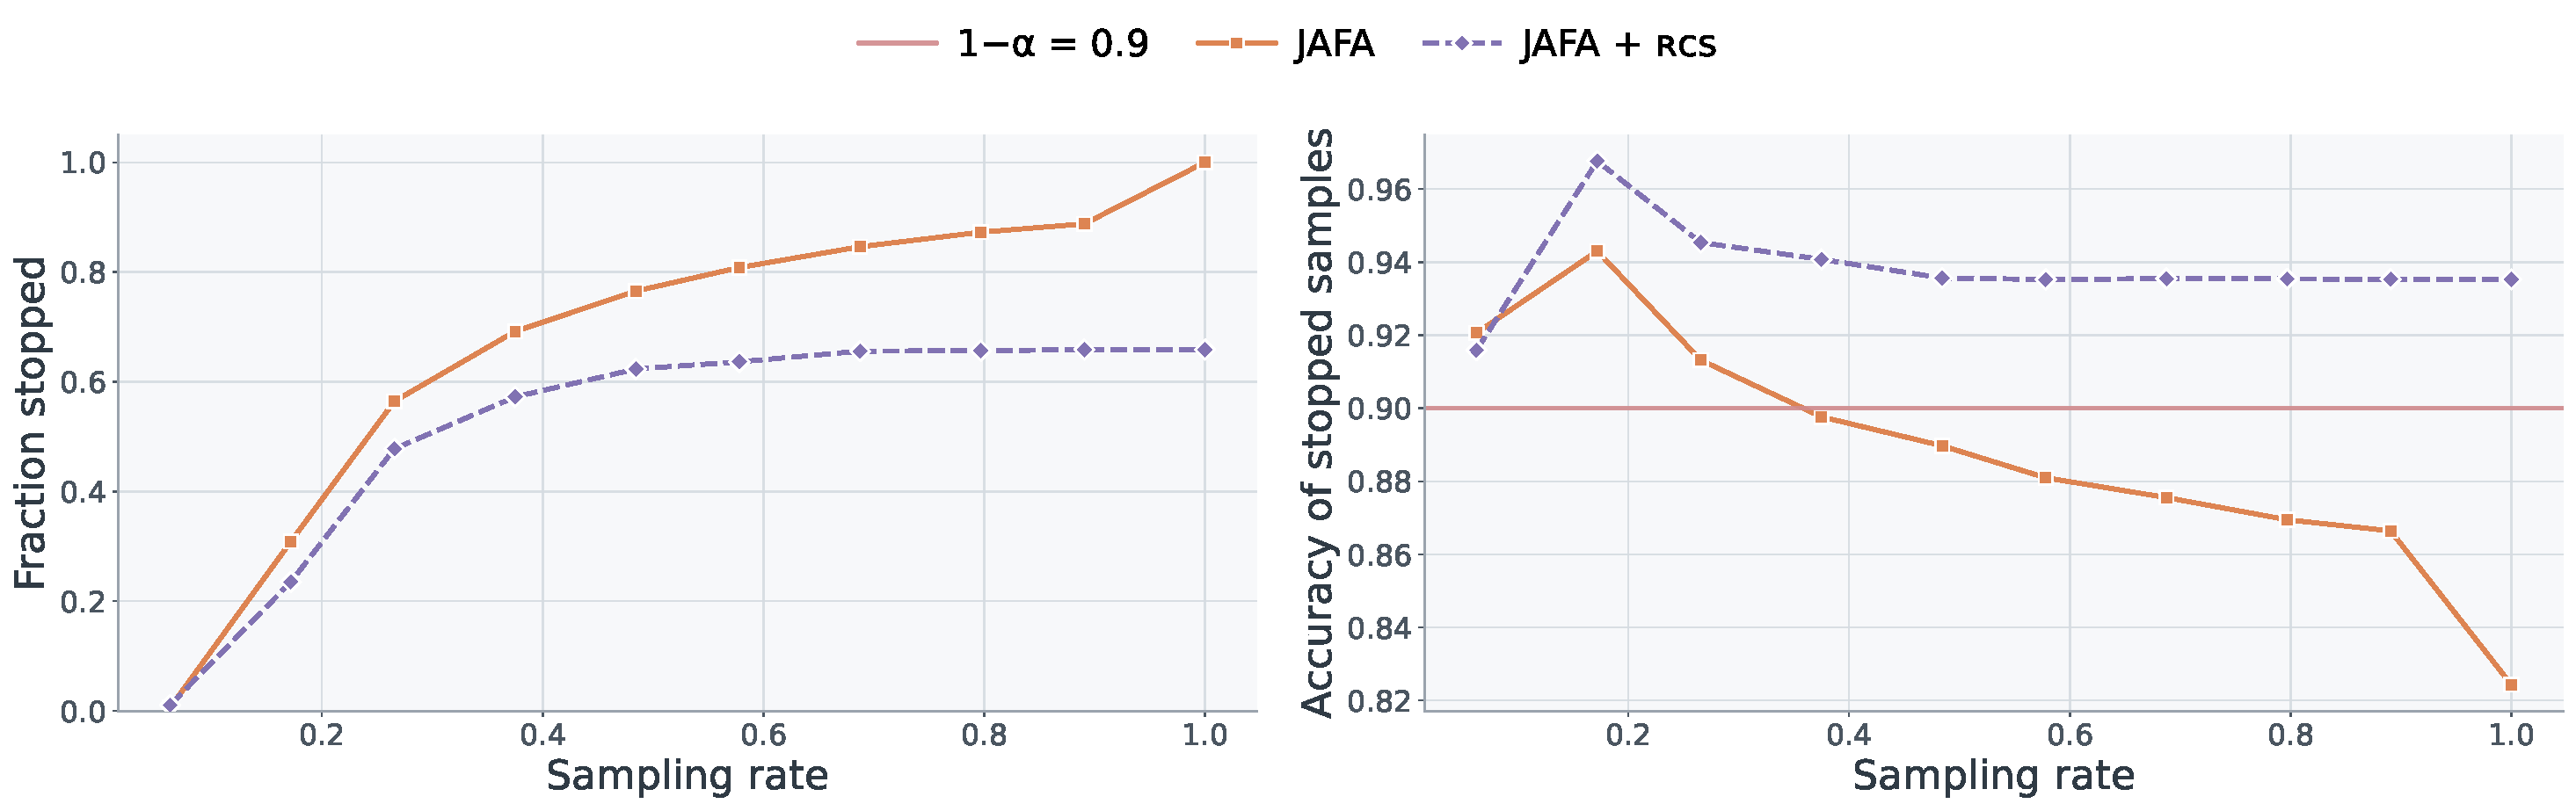
\includegraphics[width=0.9\linewidth]{figures/compare_panel_max_score_q_margin_max.pdf}}
    
    \caption{
      {\bf Upper Panel:} \textbf{Effect of the risk level $\alpha$ on calibrated stopping (FastMRI knee and Prostate PI-RADS).}
      We show the cumulative fraction of stopped examples versus sampling rate for several values of $\alpha$
      (one curve per $\alpha$).
      {\bf Lower Panel:}
  \textbf{Complementing a learned acquisition policy with \gls{method} (CIFAR-10).} In this experiment we wrap JAFA \citep{jafa-2018} with \gls{method}, and compare the efficiency and safety of the resulting policy with JAFA alone. In the left plot, we plot the fraction of samples stopped by each procedure across acquisition stages. In the right plot, we monitor the risk (miscoverage) of both across acquisition stages. We observe that at the cost of slightly lower efficiency, JAFA+\gls{method} adheres to the safety constraint while JAFA alone does not.
      }
      \label{fig:alpha-sweep}
  \end{center}
\end{figure*}


\subsection{Compatibility with Adaptive Acquisition Policies}
\label{sec:experiments_2}
Our second set of experiments evaluate whether the proposed stopping-calibration procedures can serve as post hoc wrappers on top of learned adaptive acquisition policies. Since our method is designed to be agnostic to the acquisition mechanism itself, it should be applicable not only to fixed or random acquisition trajectories, but also to learned adaptive policies, provided that the calibration and test trajectories are sampled from the same induced distribution.
To demonstrate this, we use \textbf{JAFA} \citep{jafa-2018}, a reinforcement-learning-based adaptive feature acquisition method that jointly learns which feature to acquire next and when to stop. JAFA provides a strong representative of the adaptive acquisition literature, in which acquisition decisions are optimized for average utility or reward but are not, by themselves, equipped with post hoc statistical guarantees on the risk of the final stopped decision.

\paragraph{Wrapper construction}
We treat JAFA as an acquisition backbone and construct a parameterized stopping wrapper on top of it. Concretely, JAFA generates a sequential acquisition trajectory and exposes a stopping score at each acquisition step. Specifically, JAFA learns a Deep-Q network, that produces values for a given $(\text{state},\text{action})$ pair. The policy selects the next action by picking $a_{t+1} = \argmax_a Q(a,s_t)$, where $Q$ is the Q-network and $s$ is the state at time $t$. By taking the difference between the Q-value for the "STOP" action and the argmax action (excluding $a_{t+1} = \text{"STOP"}$), we can define a score function. We then instantiate a family of wrapped stopping policies by thresholding this score with a tunable parameter $\lambda$, and apply \gls{method} to select a risk-certified member of this wrapped family. This preserves JAFA's adaptive acquisition behavior while calibrating the final decision to satisfy a user-specified risk target.

% \begin{figure*}[h!]
%   \vskip 0.2in
%   \begin{center}
%     \centerline{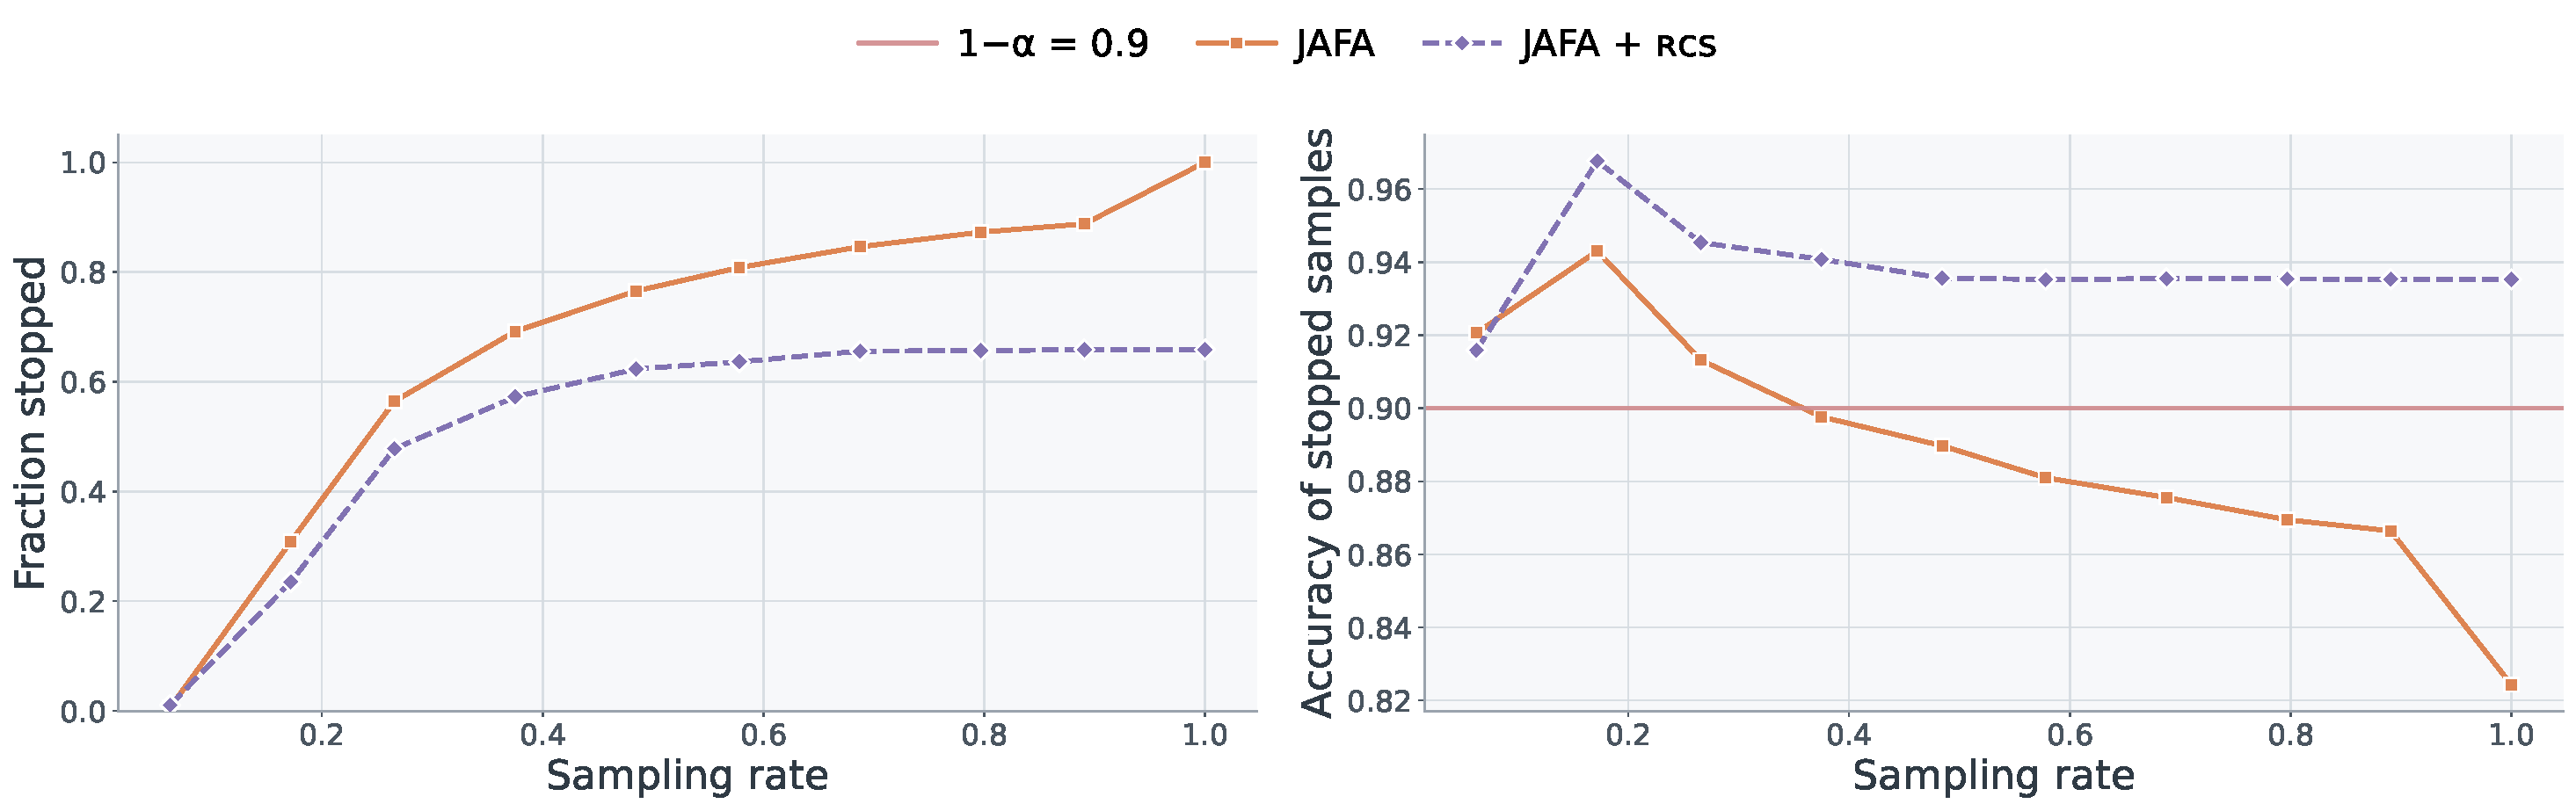
\includegraphics[width=\linewidth]{figures/compare_panel_max_score_q_margin_max.pdf}}
%     \caption{
%       \textbf{Complementing a learned acquisition policy with \gls{method}.} In this experiment we wrap JAFA \citep{jafa-2018} with \gls{method}, and compare the efficiency and safety of the resulting policy with JAFA alone. In the left plot, we plot the fraction of samples stopped by each procedure across acquisition stages. In the right plot, we monitor the risk (miscoverage) of both across acquisition stages. We observe that at the cost of slightly lower efficiency, JAFA+\gls{method} adheres to the safety constraint while JAFA alone does not.
%       }
%     \label{fig:cifar-jafa}
%   \end{center}
% \end{figure*}

\paragraph{Results.}
To isolate the effect of the wrapper cleanly, we perform this experiment on \textbf{CIFAR-10} only. As in \ref{sec:experiments_1}, we report: 1)  the cumulative fraction of stopped samples versus acquisition rate, and 2) he stopped-sample performance versus acquisition rate.
From \cref{fig:alpha-sweep} (lower panel), 
%\cref{fig:cifar-jafa}, 
we observe that calibrating on JAFA-generated acquisition trajectories enhances the efficiency of the stopping procedure. At the same time, our wrapper ensures that the accuracy of the stopped samples remains above $90\%$. Because both methods use the same underlying predictor, \gls{method} achieves this result by abstaining on the few samples that JAFA would otherwise misclassify.

\section{Discussion}
In this work, we introduce risk-controlled stopping (\textsc{rcs}), a method to safely stop data acquisition in sequential classification tasks. \gls{method} provides post-hoc, distribution-free risk control at user desired thresholds and notions of risk. These risk functions and thresholds can be changed without requiring any further training. Our experiments on the \textsc{fastMRI} knee and the prostate dataset show that \gls{method} can significantly accelerate clinical decision making pipelines, while rigorously controlling class-conditional (or stopped-sample) false-negative risk despite accelerations. Furthermore, we demonstrate that \gls{method} is complementary to learned acquisition policies, and provides rigorous statistical guarantees on their behavior. 

\subsection{Limitations}
Producing the \gls{method} guarantee requires access to fully-sampled data or data sampled from the same policy. However, in future work, we plan on using masked data that could be collected during a deployment of early stopping methods. Moreover, the class of policies parameterized by $\lambda$ could be enriched by allowing $\lambda$ to be multi-dimensional, thereby capturing the strong correlation structure among errors across nearby acquisition steps.

% ---- Statements (do not count toward the page limit) ----
% ===================== Required / recommended ICLR statements =====================
% These sections appear at the end of the main text, before references, and do
% NOT count toward the page limit.

\subsection*{Ethics statement}
This work concerns risk-controlled early stopping of medical-image acquisition. The prostate \textsc{mri} data were analyzed under an institutional IRB-approved research protocol as a retrospective study of pre-existing, de-identified clinical examinations from patients evaluated for suspected prostate cancer; no patients were enrolled and no imaging was performed for research. Splits were made at the patient level so that no patient appears in more than one of the training, validation, calibration, and test sets. \gls{method} is meant to support clinical judgment, not replace it, and any deployment would require prospective validation; in particular, faster screening can enlarge the screened population and so raise the absolute number of false positives. By design, any sample \gls{method} does not confidently stop on proceeds to the full standard-of-care protocol, so the end-to-end workflow is never less safe than current practice.

\subsection*{Reproducibility statement}
The calibration procedure is specified in \cref{sec:rcs}, with pseudocode in \cref{eq:alg_ltt} and the proof of \cref{thm:conditional_risk} in \cref{appsec:proofs}. The three policy families (confidence threshold, \textsc{jafa} Q-margin, ambiguity bands) are defined in \cref{sec:rcs} and \cref{app:ambiguity_bands}. Dataset construction, acquisition ordering, and split statistics are given in \cref{sec:experiments_1} and the appendix. \textsc{cifar}-10 and \textsc{fastMRI} are public; code for the calibration procedure and experiments will be released as anonymized supplementary material.

\subsection*{AI use statement}
% The authors used generative AI tools to edit prose for clarity and concision and to help draft the schematic in \cref{fig:rcs_figure}. 
All technical claims, proofs, experimental designs, and results were produced and verified by the authors, who reviewed and edited every AI-assisted passage and take full responsibility for the content of this work.


\bibliography{main}
\bibliographystyle{iclr2027_conference}

\appendix
\newpage
\section{Technical appendices and supplementary material}
\subsection{Proof of Risk Control}
\label{appsec:proofs}

We now briefly describe the statistical properties that lead to the guarantees underlying \gls{method}.

\paragraph{Exchangeability of sequence-level losses.}
For any fixed policy parameter, the stopping rule and terminal decision are deterministic functions of the full trajectory $X_i$. Since the calibration trajectories $(X_i,Y_i)$ are i.i.d., the induced sequence-level losses are exchangeable across samples. This allows Hoeffding's inequality to be applied to the empirical risk for each fixed candidate policy.

\paragraph{Validity of the conditional p-values.}
For the LTT procedure, the pairs $(S_i^{(j)},L_i^{(j)})$ are i.i.d. across calibration samples because each depends only on the corresponding trajectory-label pair $(X_i,Y_i)$. Conditional on the stopped index set $A_j$, the selected losses $\{L_i^{(j)}:i\in A_j\}$ remain independent. Therefore, conditional on $A_j$, the empirical conditional risk $\widehat{R}_{\mathrm{cond}}(\lambda_j)$ is the mean of $n_j$ independent $[0,1]$-valued random variables with expectation $R_{\mathrm{cond}}(\lambda_j)$ and Hoeffding's inequality yields the valid one-sided p-value \eqref{eq:hoeffding_pvalue}. Marginalizing over $A_j$ proves unconditional p-value validity.


\begin{algorithm}[H]
\caption{\gls{method}: Risk Control on Stopped Samples}
\textbf{Input:} Calibration set $\mathcal{D}_{cal}=\{(X_i,Y_i)\}_{i=1}^{n_{cal}}$, candidate grid $\Lambda=\{\lambda_1,\dots,\lambda_m\}$, target conditional risk $\alpha$, confidence level $\delta$, utility $U(\lambda)$.
\begin{algorithmic}
\FOR{$j=1,\dots,m$}
    \FOR{$i=1,\dots,n_{cal}$}
        \STATE Evaluate policy $D_{\lambda_j}$ on trajectory $X_i$ and compute stopping time
        \begin{align*}
            \tau_{\lambda_j}(X_i)=\inf\{t\in\{1,\dots,T\}:D_{\lambda_j}(X_i^t)\neq \mathrm{CONTINUE}\}
        \end{align*}
        \STATE Set
        \begin{align*}
            S_i^{(j)}=\mathbf{1}\{\tau_{\lambda_j}(X_i)<\infty\}
        \end{align*}
        \IF{$S_i^{(j)}=1$}
            \STATE Compute terminal decision
            \begin{align*}
                \hat{Y}_{\lambda_j}(X_i)=D_{\lambda_j}(X_i^{\tau_{\lambda_j}(X_i)})
            \end{align*}
            \STATE Compute loss
            \begin{align*}
                L_i^{(j)}=\mathcal{L}\bigl(\hat{Y}_{\lambda_j}(X_i),Y_i\bigr)
            \end{align*}
        \ENDIF
    \ENDFOR
    \STATE Let
    \begin{align*}
        A_j=\{i:S_i^{(j)}=1\},\qquad n_j=|A_j|
    \end{align*}
    \IF{$n_j=0$}
        \STATE Set $p_j=1$.
    \ELSE
        \STATE Compute empirical conditional risk
        \begin{align*}
            \widehat{R}_{\mathrm{cond}}(\lambda_j) = \frac{1}{n_j}\sum_{i\in A_j} L_i^{(j)}
        \end{align*}
        \STATE Compute p-value
        \begin{align*}
            p_j = \exp\!\left(-2n_j\big(\alpha-\widehat{R}_{\mathrm{cond}}(\lambda_j)\big)_+^2\right)
        \end{align*}
    \ENDIF
\ENDFOR
\STATE Apply Holm's step-down procedure to $\{p_j\}_{j=1}^m$ at level $\delta$.
\STATE Let
\begin{align*}
    \widehat{\mathcal S} = \{\lambda_j \in \Lambda : H_{0,j}\ \text{is rejected}\}
\end{align*}
\IF{$\widehat{\mathcal S}=\varnothing$}
    \STATE \textbf{return} default conservative policy or abstain.
\ELSE
    \STATE Select
    \begin{align*}
        \hat{\lambda}
        \in
        \arg\max_{\lambda_j\in\widehat{\mathcal S}} U(\lambda_j).
    \end{align*}
    \STATE \textbf{return} $\hat{\lambda}$.
\ENDIF
\end{algorithmic}\label{eq:alg_ltt}
\end{algorithm}
\newpage

\subsection{ Statistics for FastMRI Knee and Prostate Datasets}
\begin{table}[h]
\centering
\caption{Dataset statistics for \textsc{fastMRI} Knee. $N = 41,679$ slices with an approximately $80\%, 10\%, 10\%$ train/validation/test split. Patients are disjoint across partitions; the evaluated task is slice-level.}
\label{tab:fastmri_class_stats}
{%
\begin{tabular}{l|c}
\toprule
\textbf{Class Label} & \textbf{Fraction of Positive labels}  \\
\midrule
ACL Sprain      &  0.03  \\
Meniscal Tear &  0.11 \\
Abnormal        &  0.16  \\ %41679
\bottomrule
\end{tabular}
}
\end{table}


\begin{table}[h]

\centering
\caption{Clinical prostate MRI examination/volume-level split statistics. Patients are disjoint across partitions; PI-RADS positive is defined as radiologist-assigned PI-RADS $\geq 3$.}
\label{tab:prostate_dataset_stats}
{
\begin{tabular}{lcc}
\toprule
\textbf{Split} & \textbf{Total} & \textbf{Fraction of Positive Labels} \\
\midrule
Train       & 6413 & 0.48 \\
Validation  & 952  & 0.49 \\
Calibration   & 945  & 0.45 \\
Test          & 824  & 0.40 \\
\bottomrule
\end{tabular}
}
\end{table}


% =====================================================================
% Appendix: comparison with additional baselines
% Figures: figures/cifar_per_rate_lambda_test.png,
%          figures/knee_per_rate_lambda_test.png,
%          figures/prostate_per_tag_tau_test.png
% =====================================================================

\subsection{Comparison with Additional Baselines}
\label{app:baselines}

We compare \gls{method} with two more stopping baselines on all three tasks, using the same calibration and test splits and the same target level $\alpha = 0.1$ as in \cref{sec:experiments_1}. In the figures, \emph{LTT} denotes \gls{method}. Each figure follows the same layout. The \textbf{left panel} shows the cumulative fraction of test samples on which acquisition has stopped. The \textbf{remaining panels} show the risk among the stopped samples, and the horizontal line marks the target.

\paragraph{Baselines.}
\textbf{Operating Point Method:} At each acquisition time, we select a threshold on the calibration set to target empirical task-specific risk $\alpha$ across all calibration samples.
\textbf{Selective Inference:} At each acquisition time, we similarly select a threshold on the calibration set, but evaluate empirical risk only among the samples selected for early stopping. The risk is misclassification on \textsc{cifar}-10 and class-conditional \textsc{fnr} for the MRI tasks. Both baselines use the same calibration and test splits as \gls{method}, with nominal target $\alpha=0.1$. Neither empirical threshold-selection procedure, as implemented here, provides the finite-sample risk certificate of \gls{method}.

% ---------------------------------------------------------------------
\paragraph{CIFAR-10.}
\Cref{fig:app_baselines_cifar} reports the accuracy among stopped samples, with target $1-\alpha = 0.9$. The Operating Point Method stops the most samples (from about $25\%$ at a $10\%$ sampling rate to about $90\%$ at full acquisition), but its stopped-sample accuracy stays between $0.68$ and $0.74$, far below the target. Selective Inference stops no samples at a $10\%$ sampling rate and reaches $0.92$ accuracy at $20\%$. From $30\%$ onward its accuracy falls below the target, ending near $0.84$. \gls{method} stops fewer samples (about $52\%$ by full acquisition). Its stopped-sample accuracy is above $0.9$ from a $40\%$ sampling rate onward and ends at about $0.905$. At the two earliest rates, \gls{method}'s cumulative accuracy is below the target ($0.83$ and $0.88$) while only $7$--$16\%$ of samples have stopped. This does not contradict the policy-level guarantee, which controls conditional risk among all eventually stopped samples, rather than simultaneously for each intermediate cumulative stopping set $\{\tau_\lambda \leq t\}$. Checkpoint-level accuracies are therefore empirical diagnostics, not separately certified bounds. By the final acquisition stage, stopped-sample accuracy reaches about $0.905$, consistent with the target.

\begin{figure}[H]
    \centering
    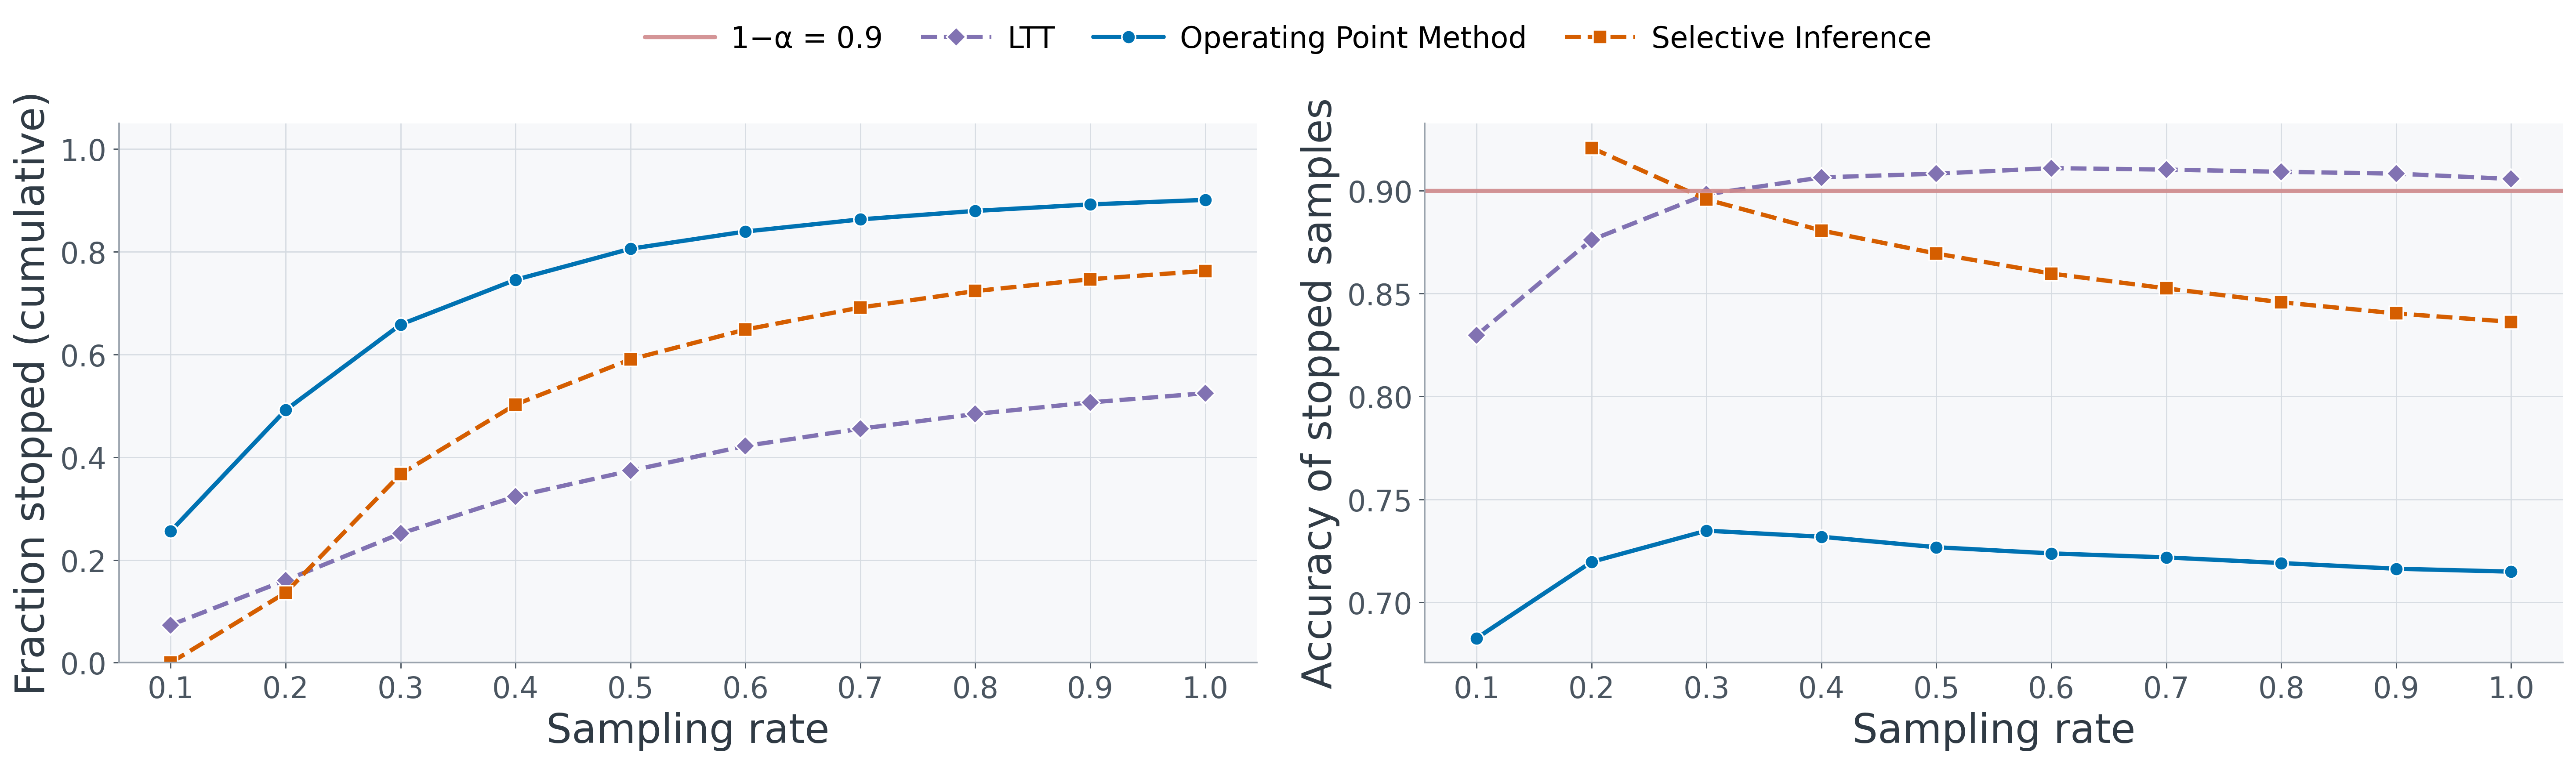
\includegraphics[width=\linewidth]{figures/cifar_per_rate_lambda_test.png}
    \caption{\textbf{Baseline comparison on \textsc{cifar}-10 ($\alpha = 0.1$).}
    \textbf{Left:} cumulative fraction of samples stopped against sampling rate.
    \textbf{Right:} accuracy among stopped samples; the horizontal line marks the target $1-\alpha = 0.9$.}
    \label{fig:app_baselines_cifar}
\end{figure}

% ---------------------------------------------------------------------
\paragraph{FastMRI knee.}
\Cref{fig:app_baselines_knee} reports the class-conditional \textsc{fnr} among stopped positives, separately for \textsc{acl} tear and meniscus tear. The Operating Point Method stops $45$--$81\%$ of slices, but its \textsc{fnr} is $0.19$--$0.23$ for \textsc{acl} and $0.25$--$0.28$ for meniscus tears, two to three times the target. Selective Inference stays within the target ($\textsc{fnr} \le 0.03$ for \textsc{acl} and $\le 0.065$ for meniscus) but stops no slices at the $5\%$ and $8\%$ sampling rates. From $12.5\%$ onward it stops more slices than \gls{method} (up to $57\%$ at $25\%$). \gls{method} is the only method that stops slices at the lowest rates while staying within the target. It stops $13\%$ of slices at $5\%$ sampling and $37\%$ at $25\%$, with an \textsc{acl} \textsc{fnr} of $0$ and a meniscus \textsc{fnr} of at most $0.012$.

\begin{figure}[H]
    \centering
    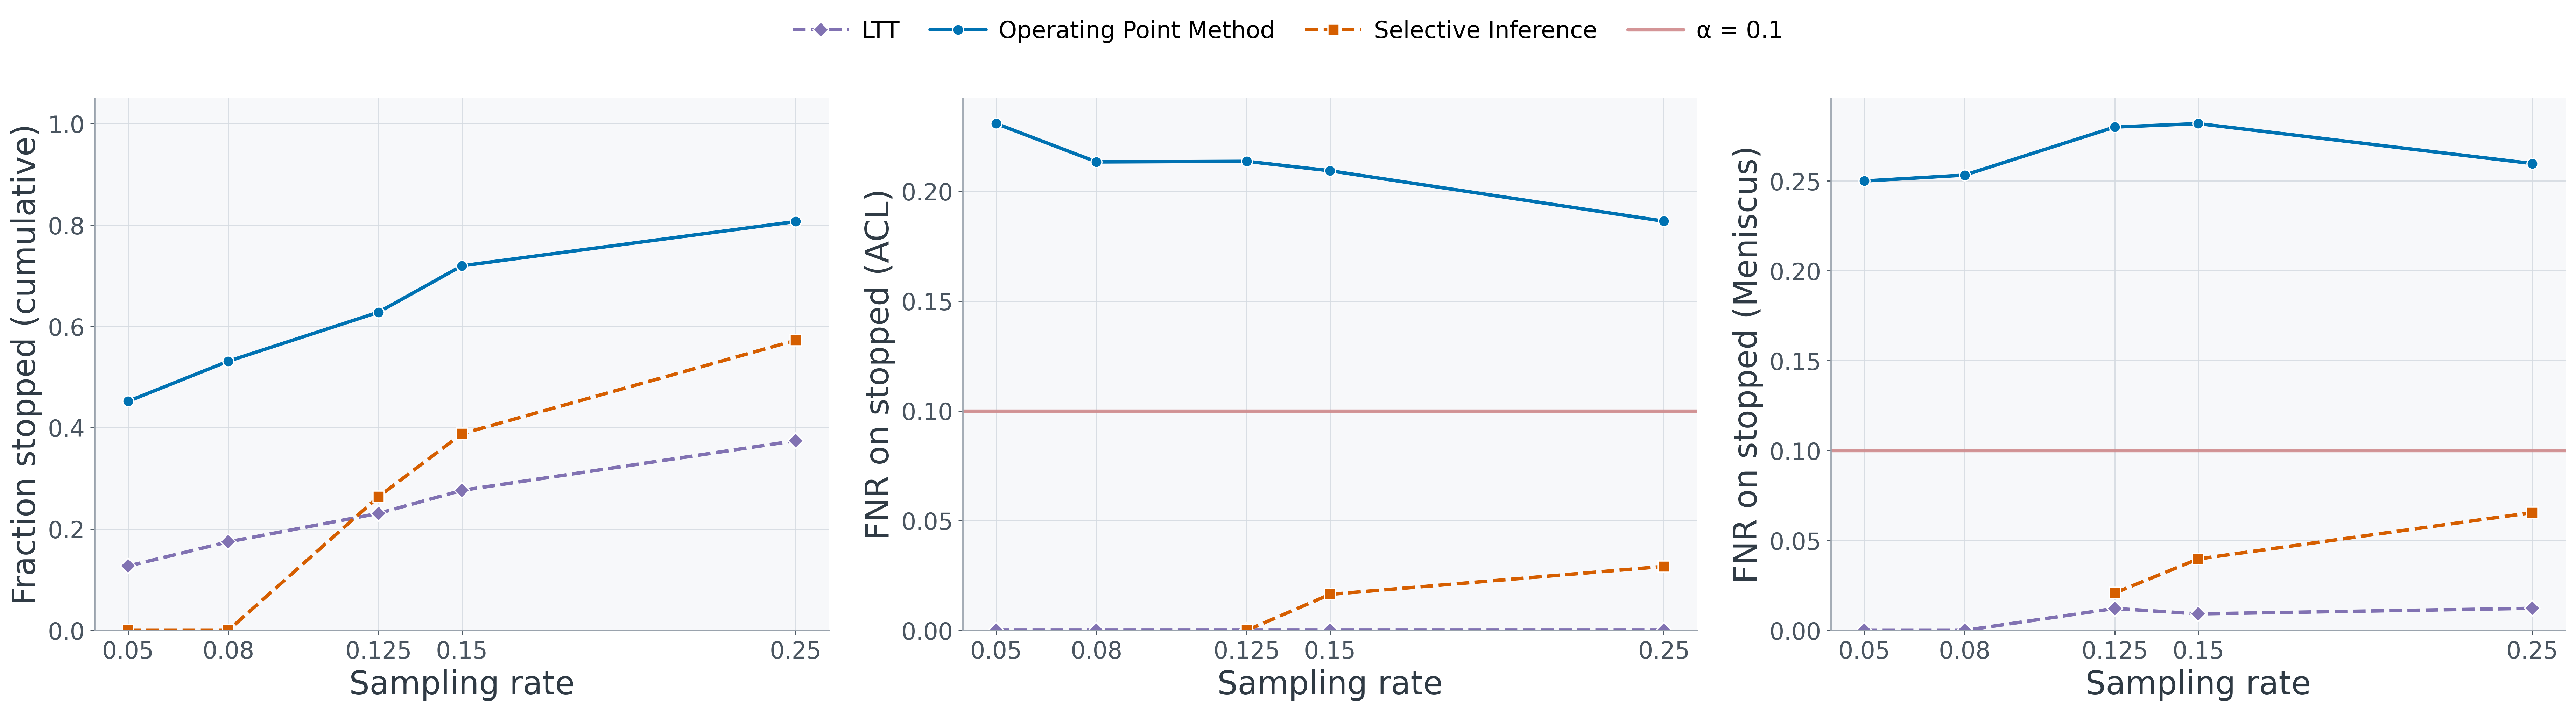
\includegraphics[width=\linewidth]{figures/knee_per_rate_lambda_test.png}
    \caption{\textbf{Baseline comparison on \textsc{fastMRI} knee ($\alpha = 0.1$).}
    \textbf{Left:} cumulative fraction of slices stopped against sampling rate.
    \textbf{Center:} \textsc{fnr} among stopped \textsc{acl}-tear positives.
    \textbf{Right:} \textsc{fnr} among stopped meniscus-tear positives.
    The horizontal line marks the target $\alpha = 0.1$.}
    \label{fig:app_baselines_knee}
\end{figure}

% ---------------------------------------------------------------------
\paragraph{Clinical prostate MRI.}
\Cref{fig:app_baselines_prostate} reports the \textsc{fnr} among stopped PI-RADS-positive exams across the $15$ scanner-ordered checkpoints of \cref{sec:experiments_1}. The tag \texttt{b50\_$i$\_b1000\_$j$} means that $i$ averages at $b=50$ and $j$ averages at $b=1000$ have been acquired. The Operating Point Method stops $55$--$76\%$ of exams with an \textsc{fnr} of $0.14$--$0.17$. Selective Inference stops $48$--$68\%$ of exams, but its \textsc{fnr} ($0.105$--$0.14$) is above the target at every checkpoint. \gls{method} stops fewer exams ($36$--$53\%$) and keeps the \textsc{fnr} between $0.026$ and $0.064$, below the target at every checkpoint.

\begin{figure}[H]
    \centering
    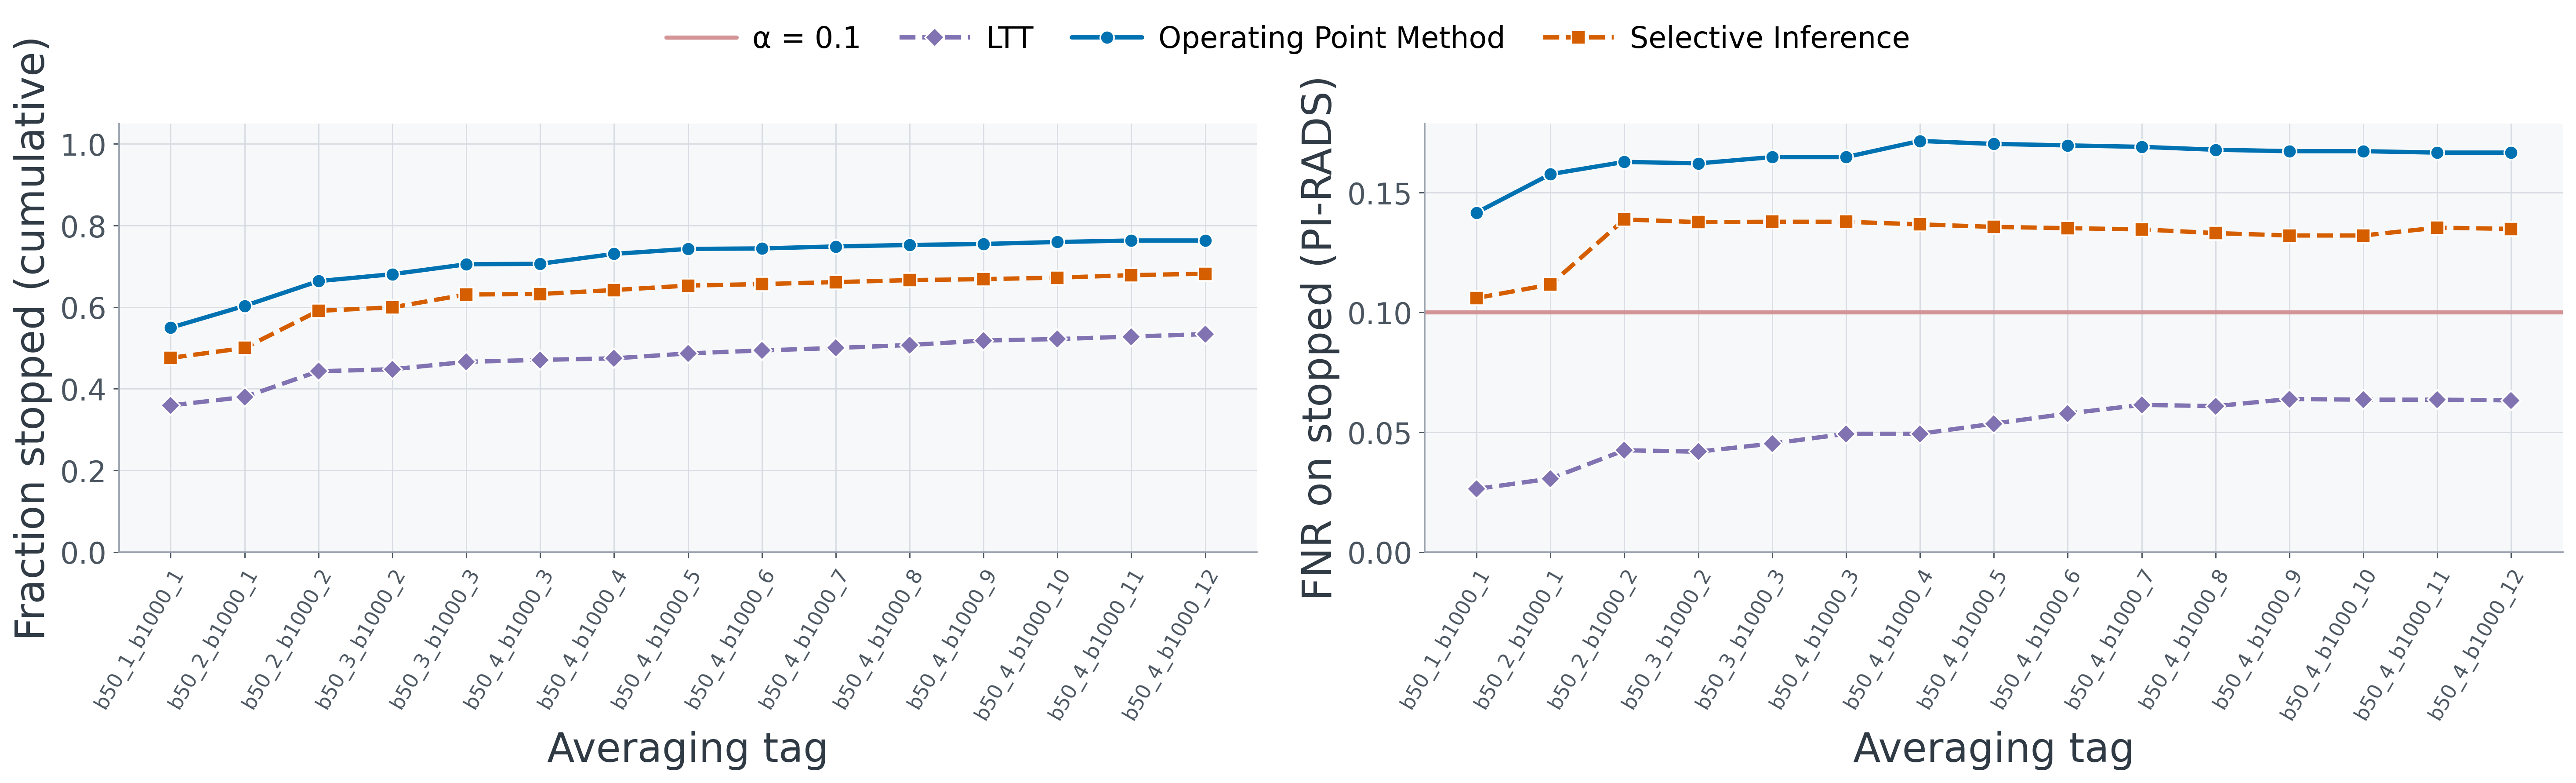
\includegraphics[width=\linewidth]{figures/prostate_per_tag_tau_test.png}
    \caption{\textbf{Baseline comparison on clinical prostate \textsc{mri} ($\alpha = 0.1$).}
    \textbf{Left:} cumulative fraction of exams stopped at each DWI checkpoint.
    \textbf{Right:} \textsc{fnr} among stopped PI-RADS-positive exams; the horizontal line marks the target $\alpha = 0.1$.
    Tags \texttt{b50\_$i$\_b1000\_$j$} give the number of $b=50$ and $b=1000$ averages acquired so far.}
    \label{fig:app_baselines_prostate}
\end{figure}

% ---------------------------------------------------------------------
\paragraph{Summary.}
The Operating Point Method stops the most samples on every task but exceeds the target risk on all three. Selective Inference stays within the target on knee but exceeds it on \textsc{cifar}-10 (from a $30\%$ sampling rate onward) and on prostate (at every checkpoint). At the final acquisition horizon, \gls{method} meets the empirical stopped-cohort risk target in all three tasks, while the two earliest \textsc{cifar}-10 checkpoint accuracies fall below the target. These intermediate measurements are not separately certified. \gls{method} generally stops fewer samples than the baselines, although the relative efficiency changes with acquisition time.
% =====================================================================
% Appendix: ablations on delta, lambda-grid density, calibration-set size
% Figures: figures/ablation_cifar_all.png,
%          figures/ablation_knee_all.png,
%          figures/ablation_prostate_all.png
% =====================================================================

\subsection{Sensitivity to Calibration Hyperparameters}
\label{app:ablations}

\gls{method} has three calibration hyper-parameters: the significance level $\delta$ of the Holm correction, the number of candidate values in the grid $\Lambda$, and the calibration set size $n_{\text{cal}}$. We vary one at a time and hold the other two at their defaults, with $\alpha = 0.1$ throughout. \Cref{fig:app_ablation_cifar,fig:app_ablation_knee,fig:app_ablation_prostate} share one layout. Row~(a) varies $\delta$, row~(b) varies the grid size, and row~(c) varies $n_{\text{cal}}$. Within each row, the left panel shows the cumulative fraction of test samples stopped and the remaining panels show the risk among stopped samples. The thick black curve is the default setting. Each legend entry gives the selected parameter $\hat\lambda$, or states that no $\lambda$ was certified, in which case \gls{method} stops no samples and every sample is fully acquired. Settings that select the same $\hat\lambda$ give identical curves and share one legend entry.

\paragraph{CIFAR-10.}
The defaults are $\delta = 0.05$, a grid of $101$ values and $n_{\text{cal}} = 4800$, which select $\hat\lambda = 0.94$ (\cref{fig:app_ablation_cifar}). For this policy family, a larger $\lambda$ is a stricter confidence threshold.
\textbf{(a)} The result barely depends on $\delta$. $\delta \in \{0.05, 0.1, 0.2\}$ all select $\hat\lambda = 0.94$. The stricter $\delta \in \{0.01, 0.025\}$ select $\hat\lambda = 0.95$, which stops slightly fewer samples ($50\%$ vs.\ $52\%$ at full acquisition) with slightly higher final accuracy ($0.914$ vs.\ $0.906$).
\textbf{(b)} Grids of $21$ to $501$ values select $\hat\lambda$ between $0.94$ and $0.95$, with nearly identical curves. The coarsest grid ($11$ values, step $0.1$) certifies no $\lambda$, because it contains no value between the unsafe region and the trivially conservative end of the grid.
\textbf{(c)} The calibration set size matters most. With $n_{\text{cal}} \in \{250, 500, 1000\}$, no $\lambda$ is certified. With $n_{\text{cal}} = 2000$, \gls{method} certifies the more conservative $\hat\lambda = 0.98$. This stops $39\%$ of samples by full acquisition (vs.\ $52\%$ at the default), with final accuracy $0.94$.
In every certified setting, the stopped-sample accuracy is above $0.9$ from a $30$--$40\%$ sampling rate onward. At the two earliest rates it is below the target, as in \cref{app:baselines}.

\begin{figure}[H]
    \centering
    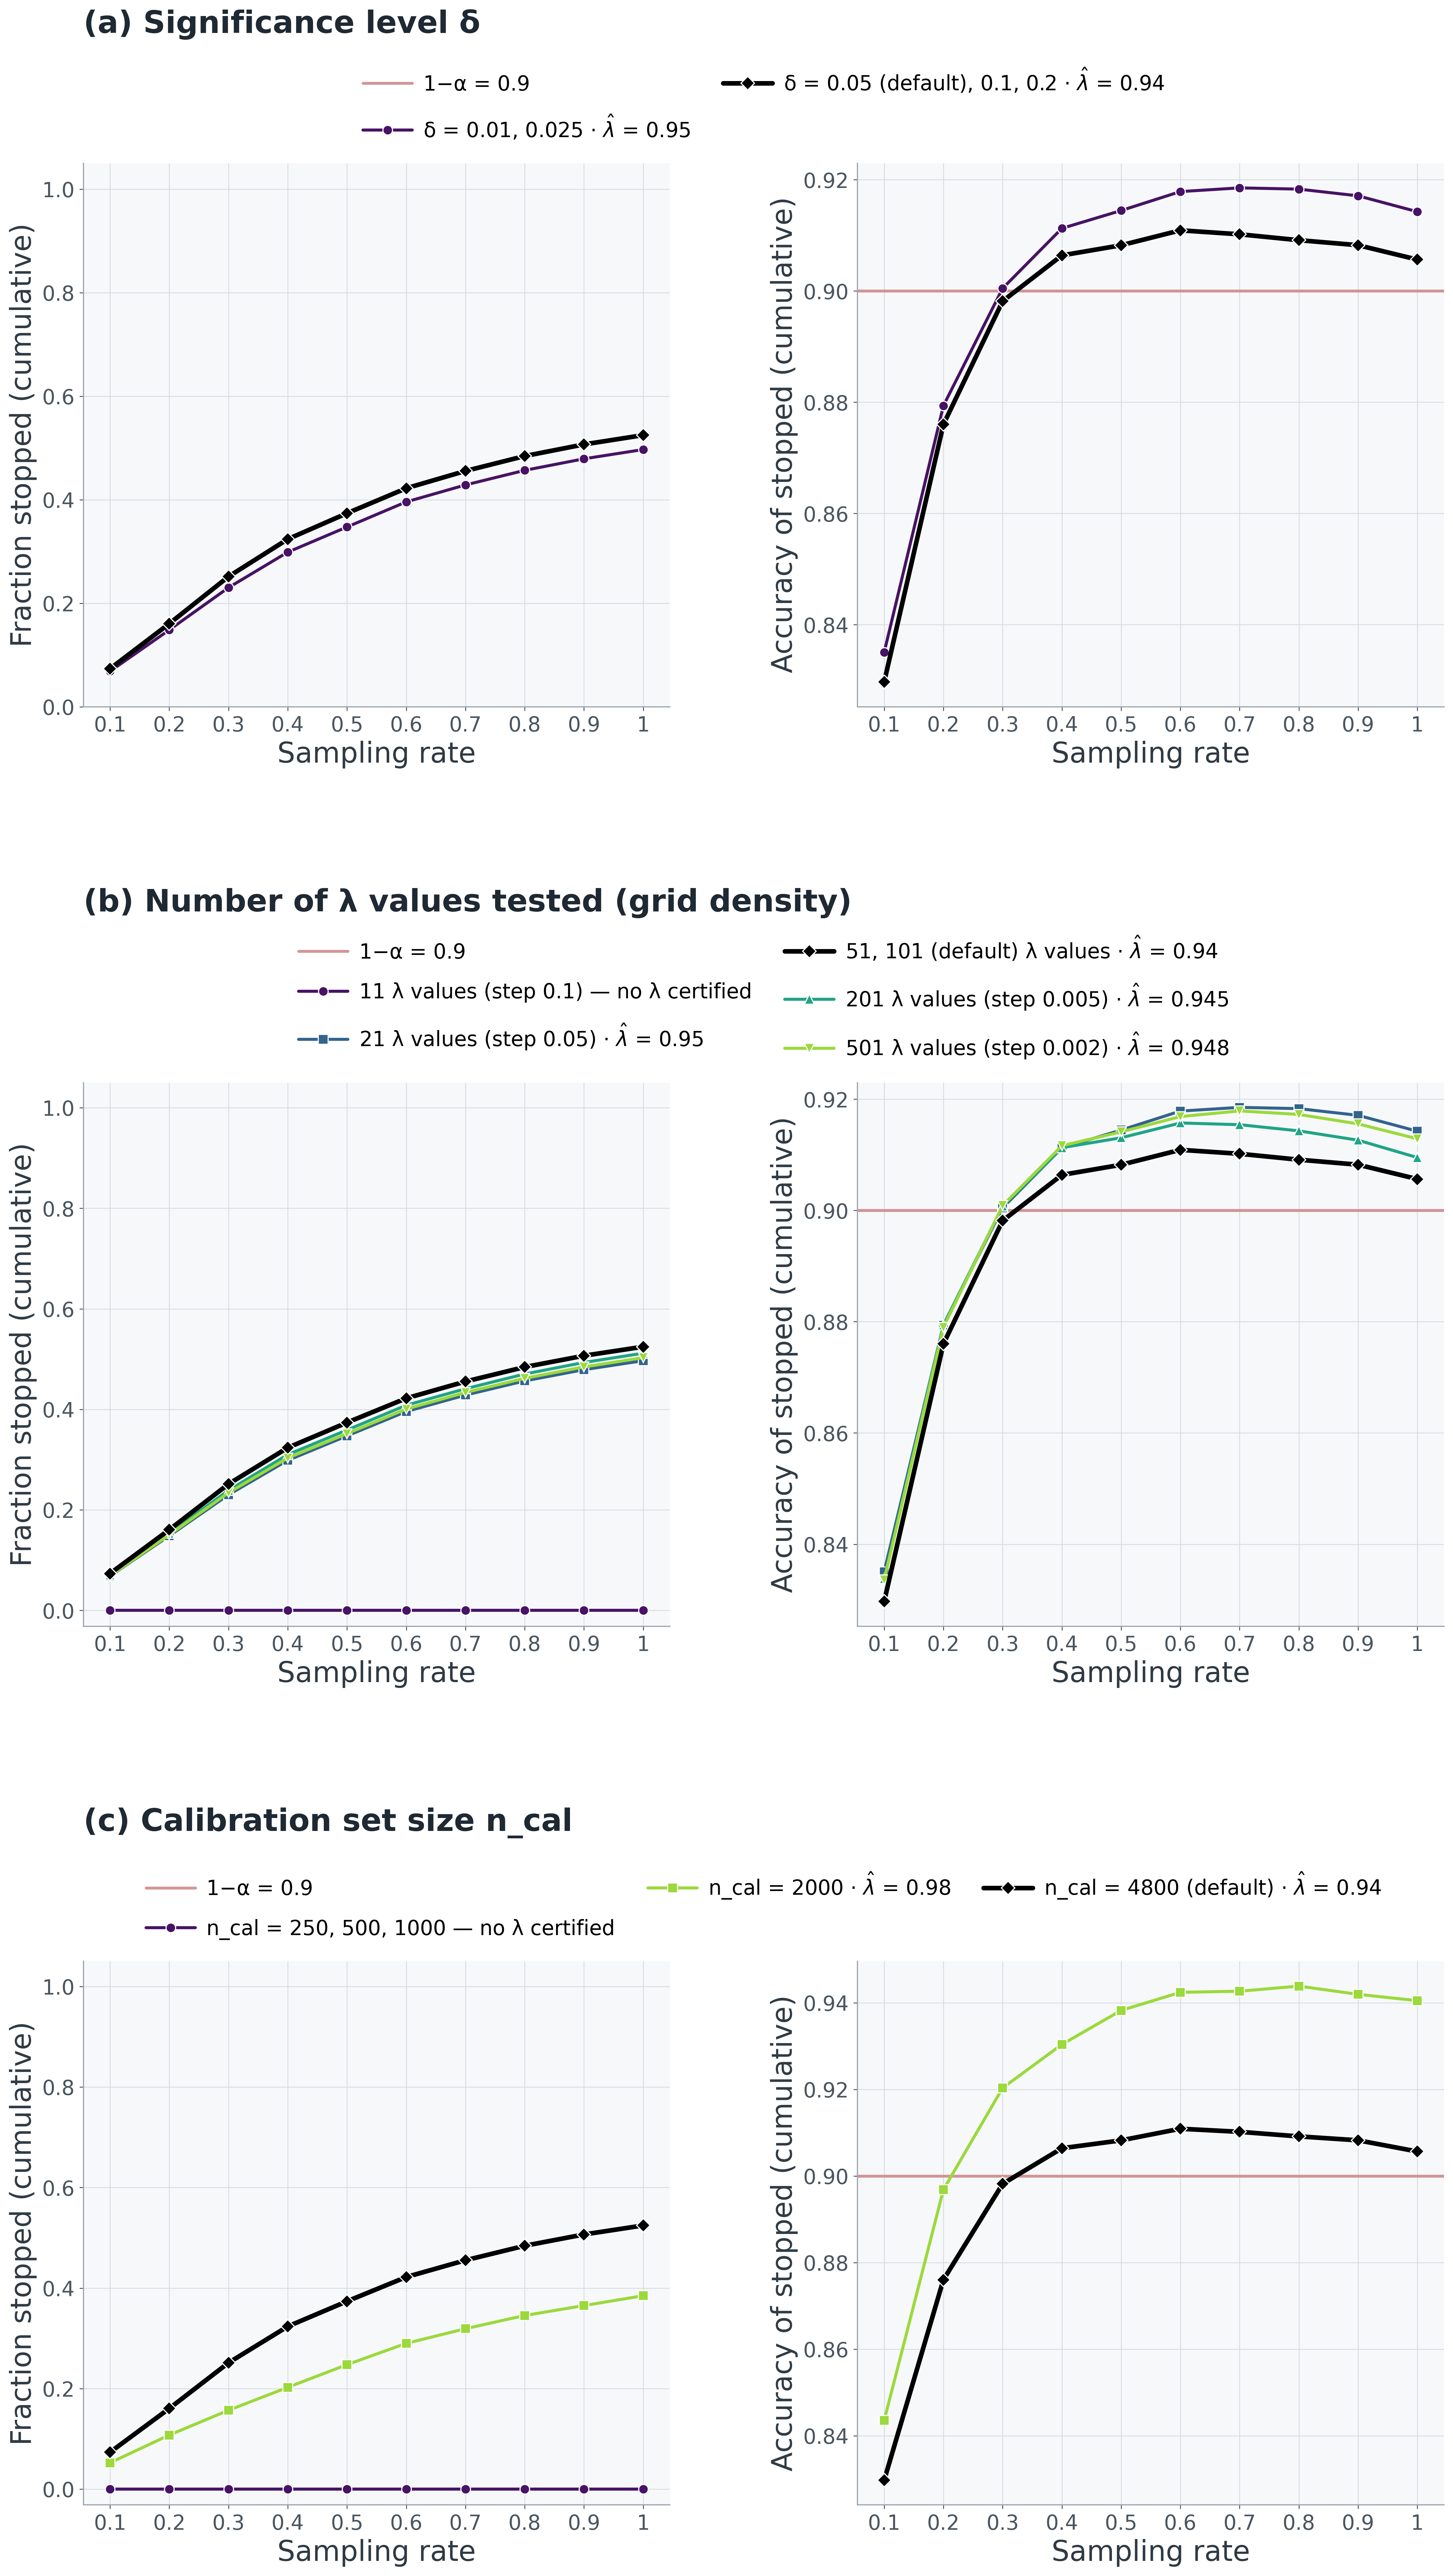
\includegraphics[width=\linewidth,height=0.8\textheight,keepaspectratio]{figures/ablation_cifar_all.png}
    \caption{\textbf{Hyperparameter sensitivity on \textsc{cifar}-10 ($\alpha = 0.1$).}
    \textbf{(a)} Significance level $\delta$.
    \textbf{(b)} Number of $\lambda$ values in the grid.
    \textbf{(c)} Calibration set size $n_{\text{cal}}$.
    Left: cumulative fraction of samples stopped. Right: accuracy among stopped samples; the horizontal line marks $1-\alpha = 0.9$. The thick black curve is the default setting.}
    \label{fig:app_ablation_cifar}
\end{figure}

% ---------------------------------------------------------------------
\paragraph{FastMRI knee.}
The defaults are $\delta = 0.1$, a grid of $15$ values and $n_{\text{cal}} = 6180$, which select $\hat\lambda = 0.4286$ (\cref{fig:app_ablation_knee}). For the ambiguity bands, a larger $\lambda$ is a narrower band and more aggressive stopping.
\textbf{(a)} $\delta = 0.01$ certifies no $\lambda$. The other levels select $\hat\lambda$ between $0.36$ and $0.5$. Every resulting policy keeps both pathology-specific \textsc{fnr}s at or below $0.044$, well under the target. The selected thresholds differ across evaluated significance levels; these values describe the reported sensitivity sweep and do not establish a general monotone relationship between $\delta$ and the selected threshold.
\textbf{(b)} Grid sizes from $3$ to $113$ select $\hat\lambda$ between $0.43$ and $0.51$. The stopped fraction at a $25\%$ sampling rate ranges from $37\%$ to $46\%$, and the \textsc{fnr} stays at or below $0.05$ for both pathologies.
\textbf{(c)} Only the full calibration set certifies a $\lambda$. With $n_{\text{cal}} \in \{500, 1000, 2000, 4000\}$, no $\lambda$ is certified. These subsets contain only $12$--$93$ \textsc{acl}-tear positives, too few to certify an \textsc{fnr} bound for this rare pathology. \gls{method} then certifies no early-stopping candidate and defers every slice to full acquisition.

\begin{figure}[H]
    \centering
    \includegraphics[width=\linewidth,height=0.8\textheight,keepaspectratio]{figures/ablation_knee_all.png}
    \caption{\textbf{Hyperparameter sensitivity on \textsc{fastMRI} knee ($\alpha = 0.1$).}
    \textbf{(a)} Significance level $\delta$.
    \textbf{(b)} Number of $\lambda$ values in the grid.
    \textbf{(c)} Calibration set size $n_{\text{cal}}$; the legend gives the number of \textsc{acl}-tear and meniscus-tear positives in each calibration set.
    Left: cumulative fraction of slices stopped. Center/Right: \textsc{fnr} among stopped \textsc{acl}-tear and meniscus-tear positives; the horizontal line marks $\alpha = 0.1$. The thick black curve is the default setting.}
    \label{fig:app_ablation_knee}
\end{figure}

% ---------------------------------------------------------------------
\paragraph{Clinical prostate MRI.}
The defaults are $\delta = 0.1$, a grid of $51$ values and $n_{\text{cal}} = 745$, which select $\hat\lambda = 0.58$ (\cref{fig:app_ablation_prostate}). Of the $945$ examinations in the calibration partition reported in \cref{tab:prostate_dataset_stats}, $745$ are used for risk calibration. The remaining $200$ examinations were unused in these experiments, including for ambiguity-band estimation.
\textbf{(a)} $\delta \in \{0.01, 0.025, 0.05, 0.1\}$ all select $\hat\lambda = 0.58$. $\delta = 0.2$ selects $\hat\lambda = 0.6$, which stops about $4$ percentage points more exams and has an \textsc{fnr} of at most $0.077$.
\textbf{(b)} Grid sizes from $6$ to $201$ select $\hat\lambda$ between $0.58$ and $0.6$. The curves differ by a few percentage points, and every \textsc{fnr} stays below $0.08$.
\textbf{(c)} With $n_{\text{cal}} \in \{100, 200\}$ ($41$ and $84$ PI-RADS-positive exams), no $\lambda$ is certified. From $n_{\text{cal}} = 400$ ($168$ positives) upward, the selection is stable at $\hat\lambda = 0.58$.

\begin{figure}[H]
    \centering
    \includegraphics[width=\linewidth,height=0.8\textheight,keepaspectratio]{figures/ablation_prostate_all.png}
    \caption{\textbf{Hyperparameter sensitivity on clinical prostate \textsc{mri} ($\alpha = 0.1$).}
    \textbf{(a)} Significance level $\delta$.
    \textbf{(b)} Number of $\lambda$ values in the grid.
    \textbf{(c)} Calibration set size $n_{\text{cal}}$; the legend gives the number of PI-RADS-positive exams in each calibration set.
    Left: cumulative fraction of exams stopped at each DWI checkpoint. Right: \textsc{fnr} among stopped PI-RADS-positive exams; the horizontal line marks $\alpha = 0.1$. The thick black curve is the default setting.}
    \label{fig:app_ablation_prostate}
\end{figure}

% ---------------------------------------------------------------------
\paragraph{Summary.}
\gls{method} is insensitive to $\delta$ and to the grid size over a wide range. Changing either moves $\hat\lambda$ only slightly, and the stopped-sample risk stays below the target in every certified setting, except at the two earliest \textsc{cifar}-10 rates. A very coarse grid can miss the safe region entirely (\textsc{cifar}-10, $11$ values). The calibration set size is the main limit. What matters is the number of calibration samples in the class whose error rate is controlled. For prostate, $84$ PI-RADS positives were too few and $168$ were enough. For knee, $93$ \textsc{acl}-tear positives were too few and the full set's $155$ were enough. Below that, \gls{method} certifies no rule and defers to full acquisition rather than returning an unsafe one.

% \begin{figure}[ht]
%     \centering
%     \begin{minipage}{0.48\textwidth}
%         \centering
%         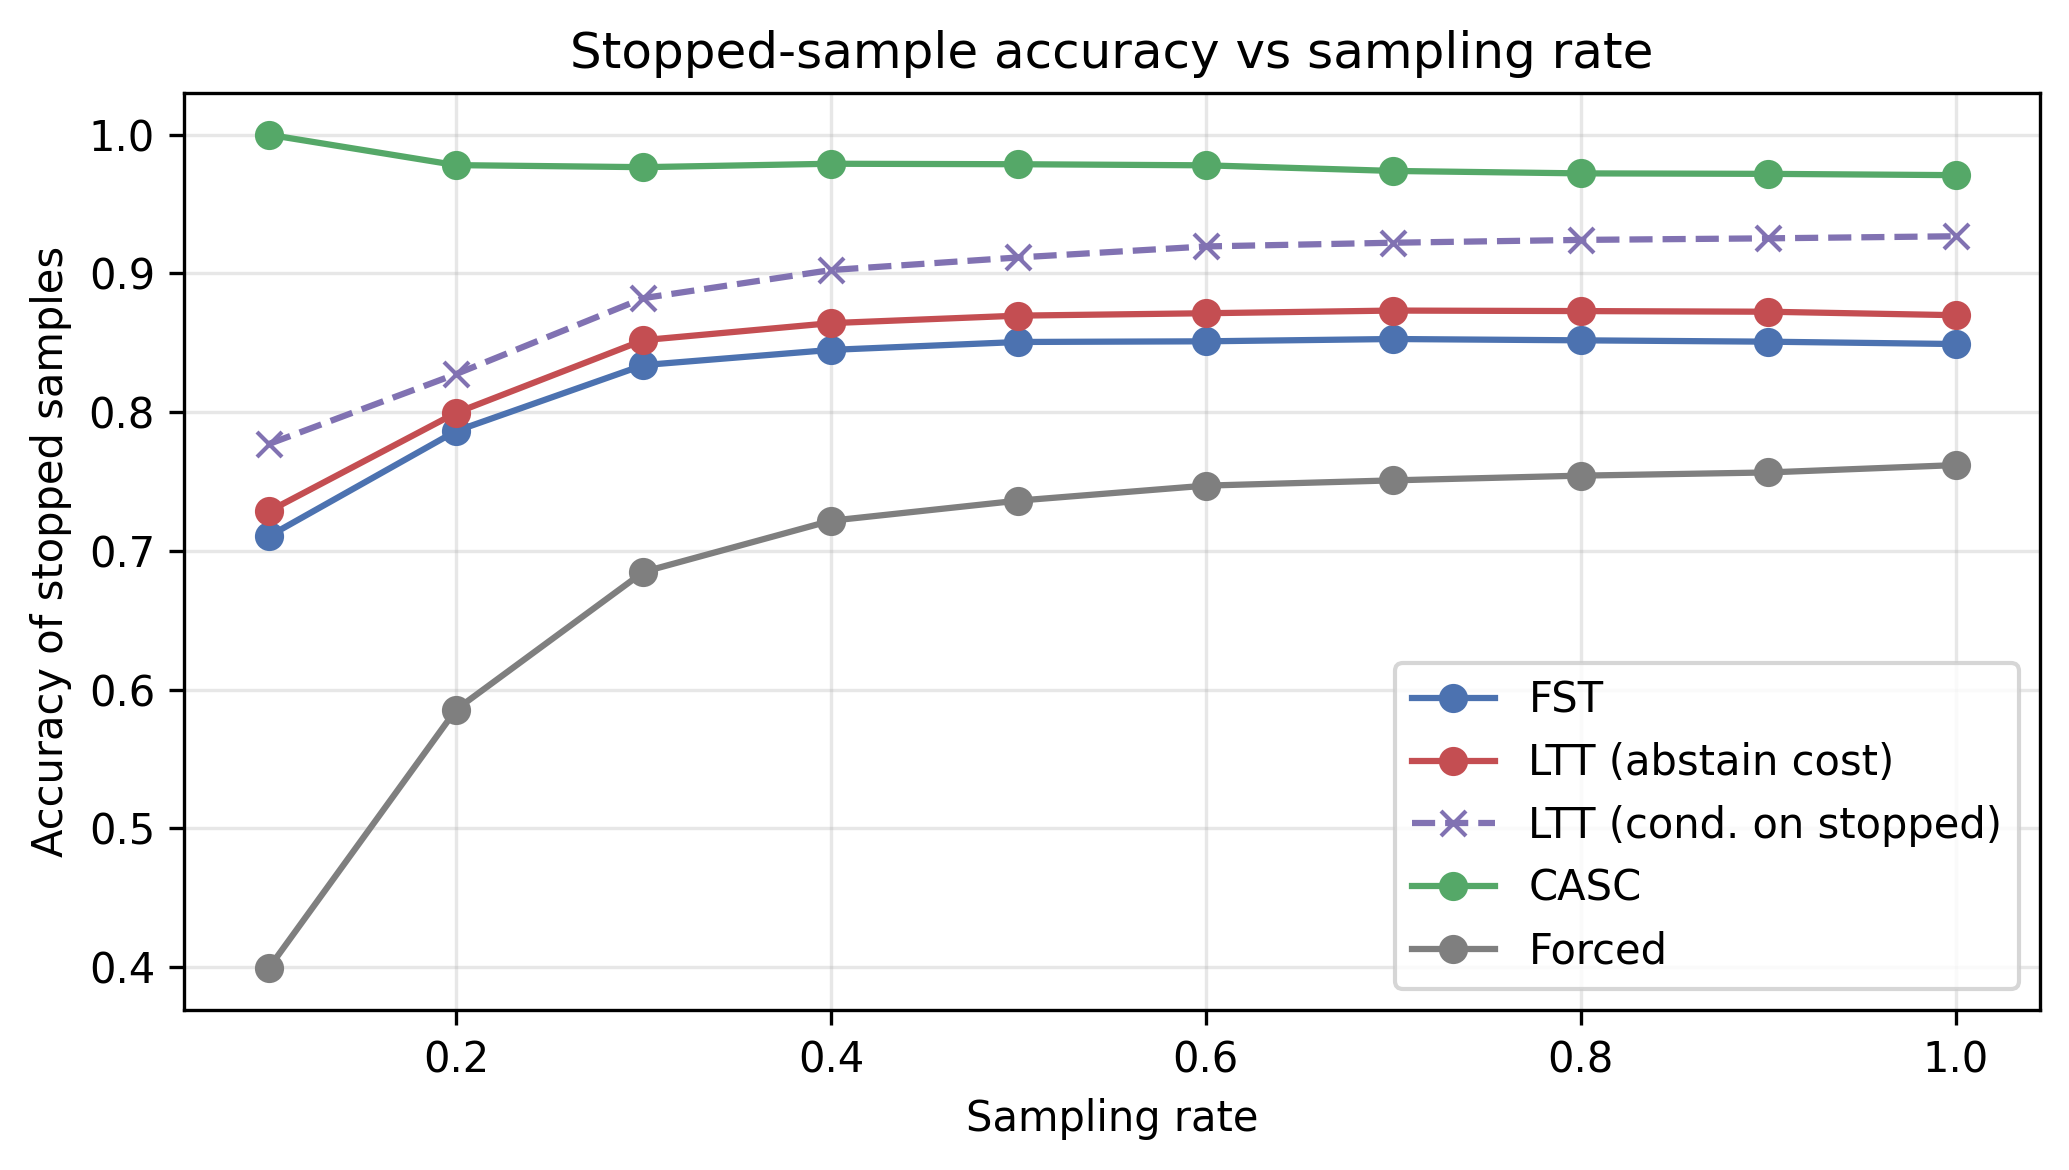
\includegraphics[width=\linewidth]{figures/cifar10_compare_stopped_accuracy_vs_sampling_rate_max_score.png}
%         \caption*{(a) \textbf{CIFAR-10} : Accuracy among stopped samples against sampling rate}
%     \end{minipage}\hfill
%     \begin{minipage}{0.48\textwidth}
%         \centering
%         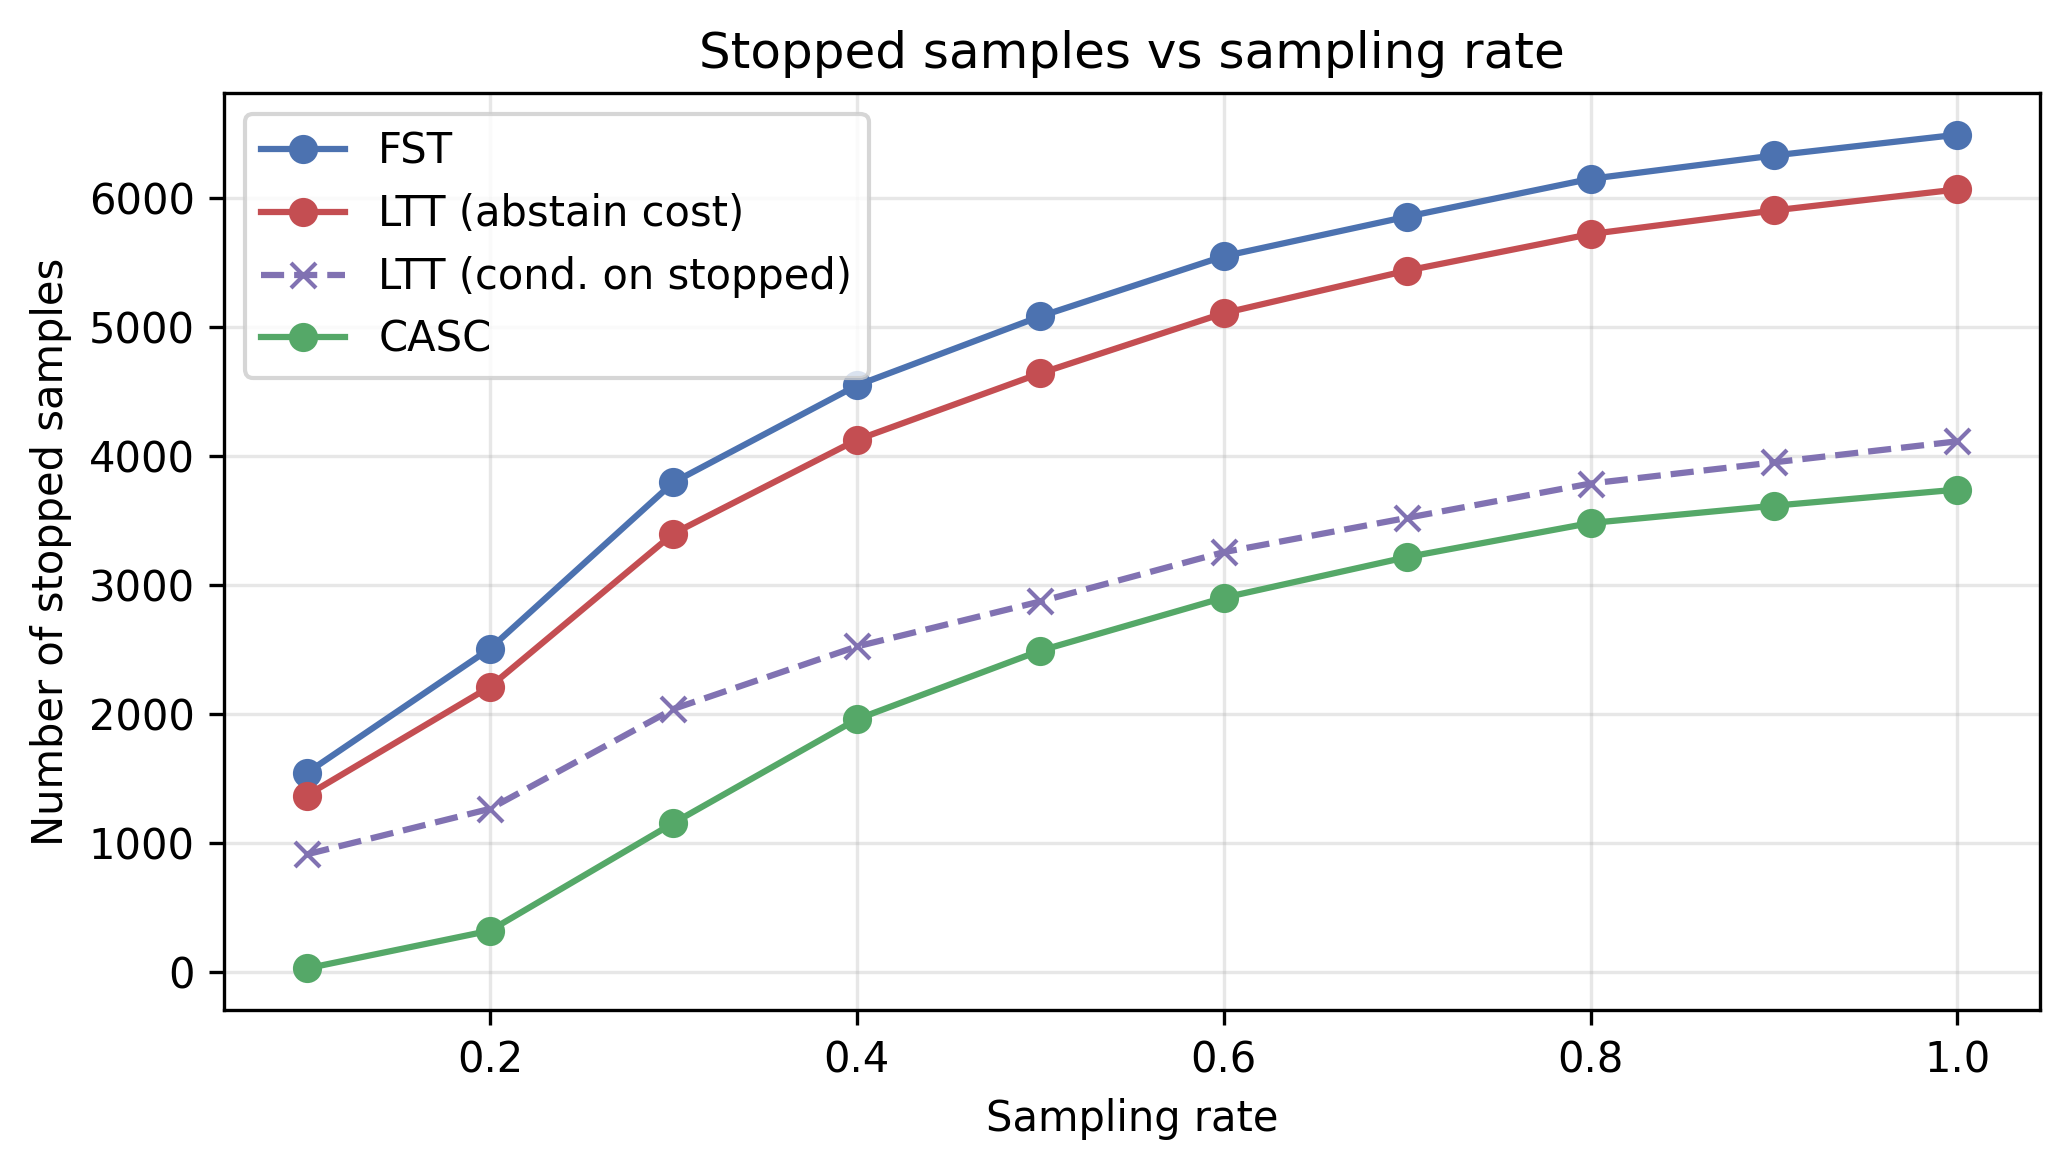
\includegraphics[width=\linewidth]{figures/cifar10_compare_stopped_vs_sampling_rate_max_score.png}
%         \caption*{\textbf{CIFAR-10} : Fraction of stopped samples against sampling rate}
%     \end{minipage}
%     \caption{CIFAR-10  Results}
%     \label{fig:two-plots}
% \end{figure}

% \begin{figure}[ht]
%     \centering
%     \begin{minipage}{0.48\textwidth}
%         \centering
%         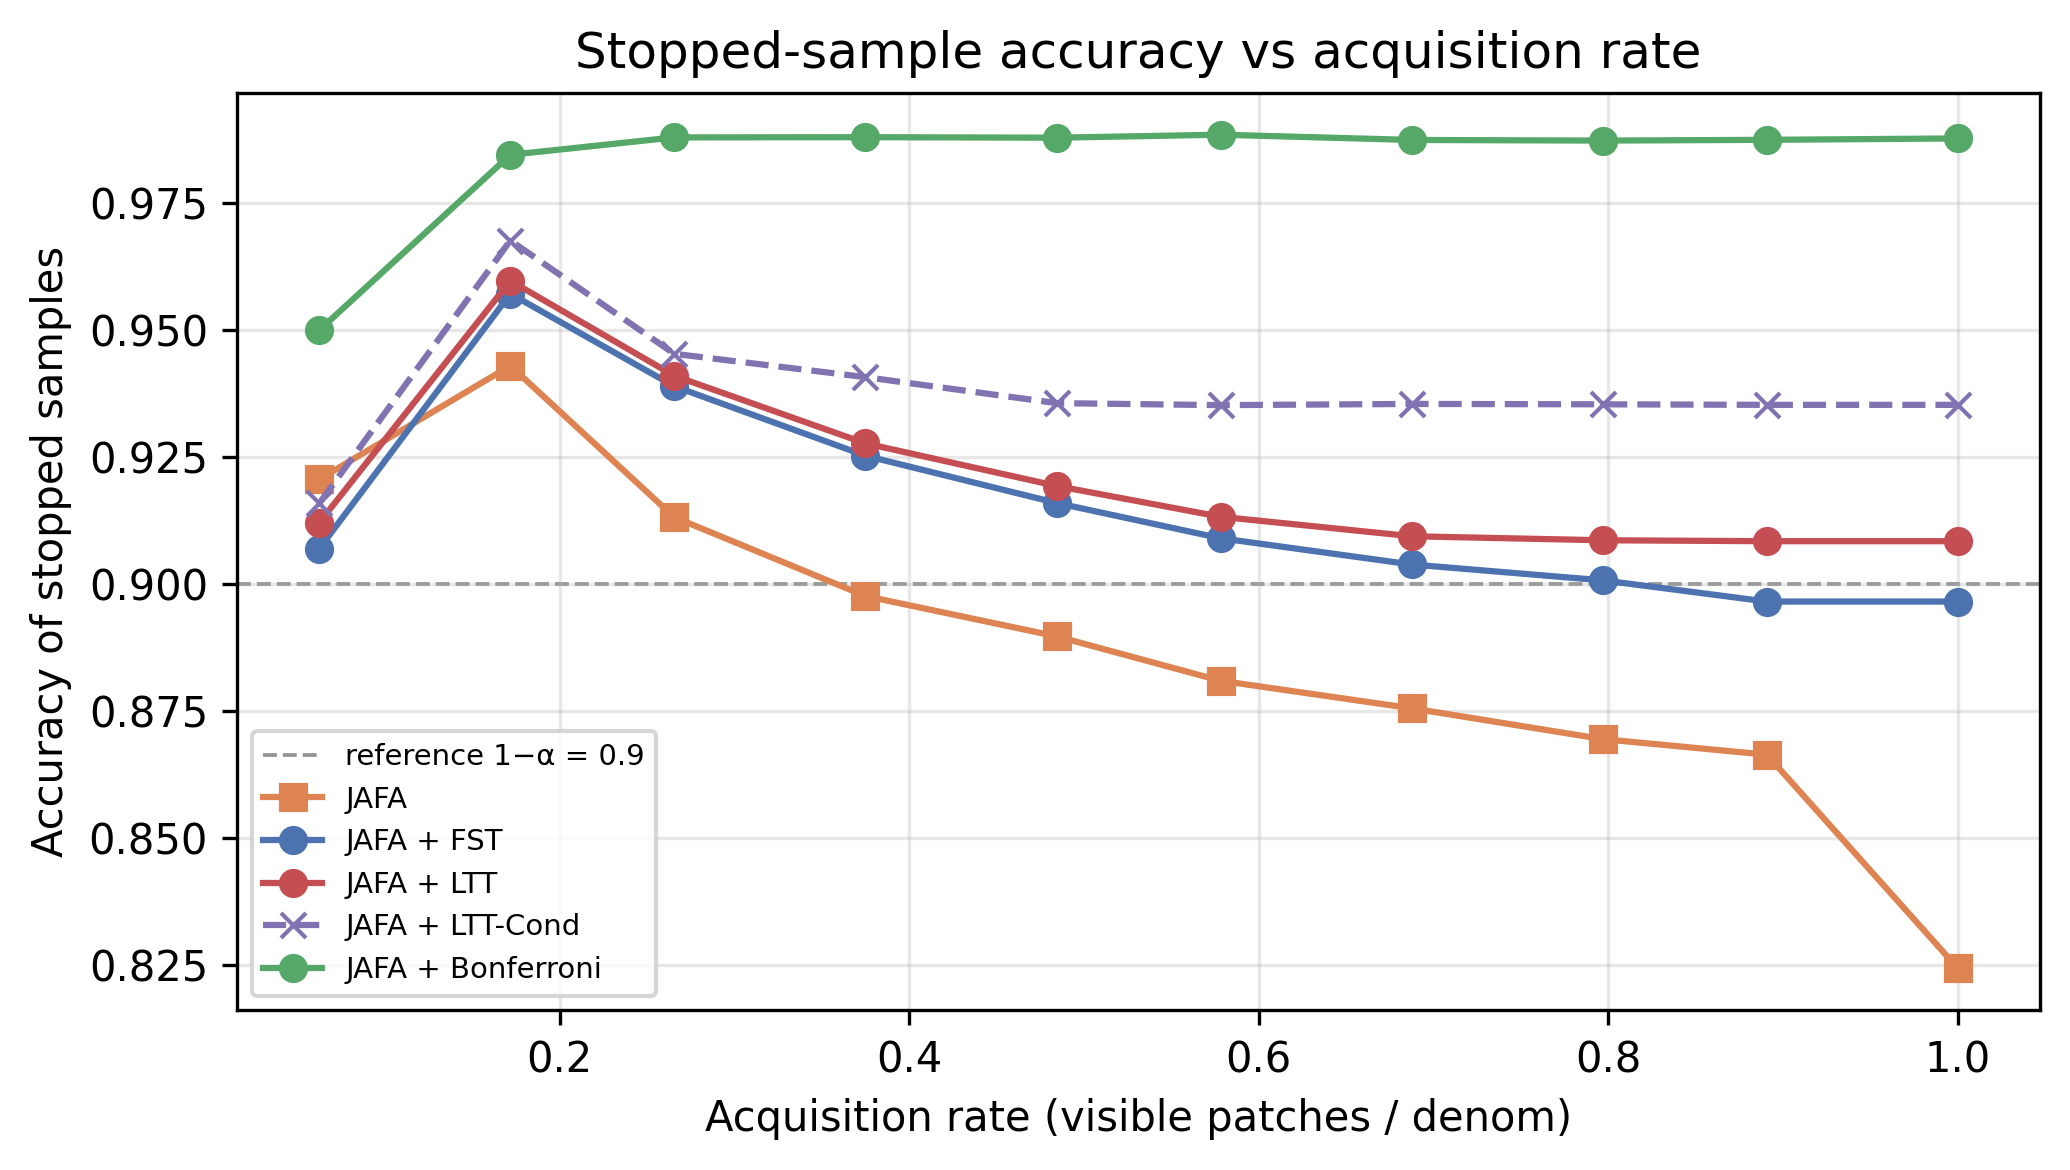
\includegraphics[width=\linewidth]{figures/compare_rl_jafa_stopped_accuracy_vs_rate_max_score_q_margin_max.png}
%         \caption*{(a) \textbf{CIFAR-10} : Accuracy among stopped samples against sampling rate}
%     \end{minipage}\hfill
%     \begin{minipage}{0.48\textwidth}
%         \centering
%         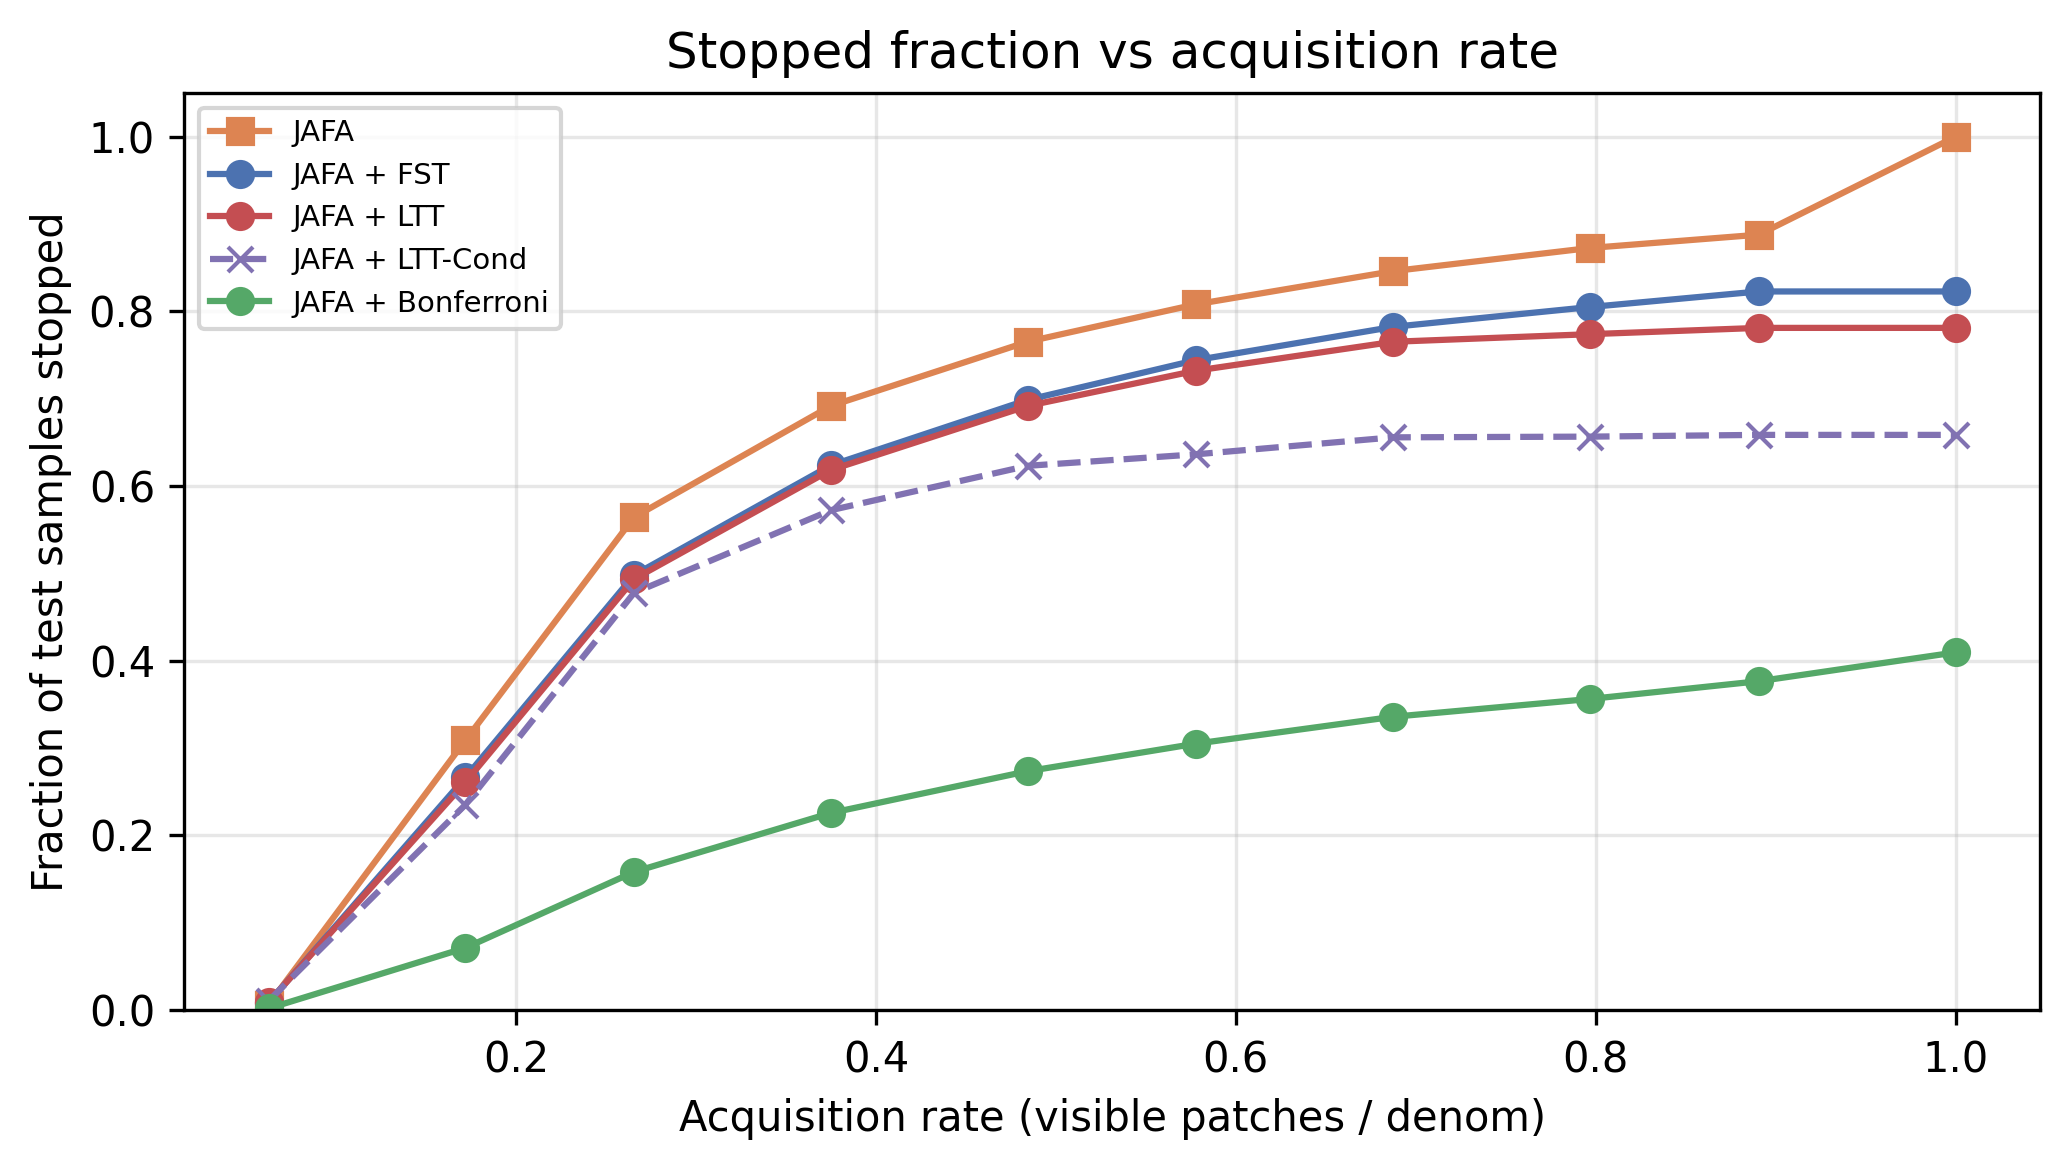
\includegraphics[width=\linewidth]{figures/compare_rl_jafa_stopped_vs_rate_max_score_q_margin_max.png}
%         \caption*{\textbf{CIFAR-10} : Fraction of stopped samples against sampling rate}
%     \end{minipage}
%     \caption{Complementing RL-based learned acquisition policies }
%     \label{fig:two-plots}
% \end{figure}

% \begin{figure}[ht]
%     \centering
%     \begin{minipage}{0.48\textwidth}
%         \centering
%         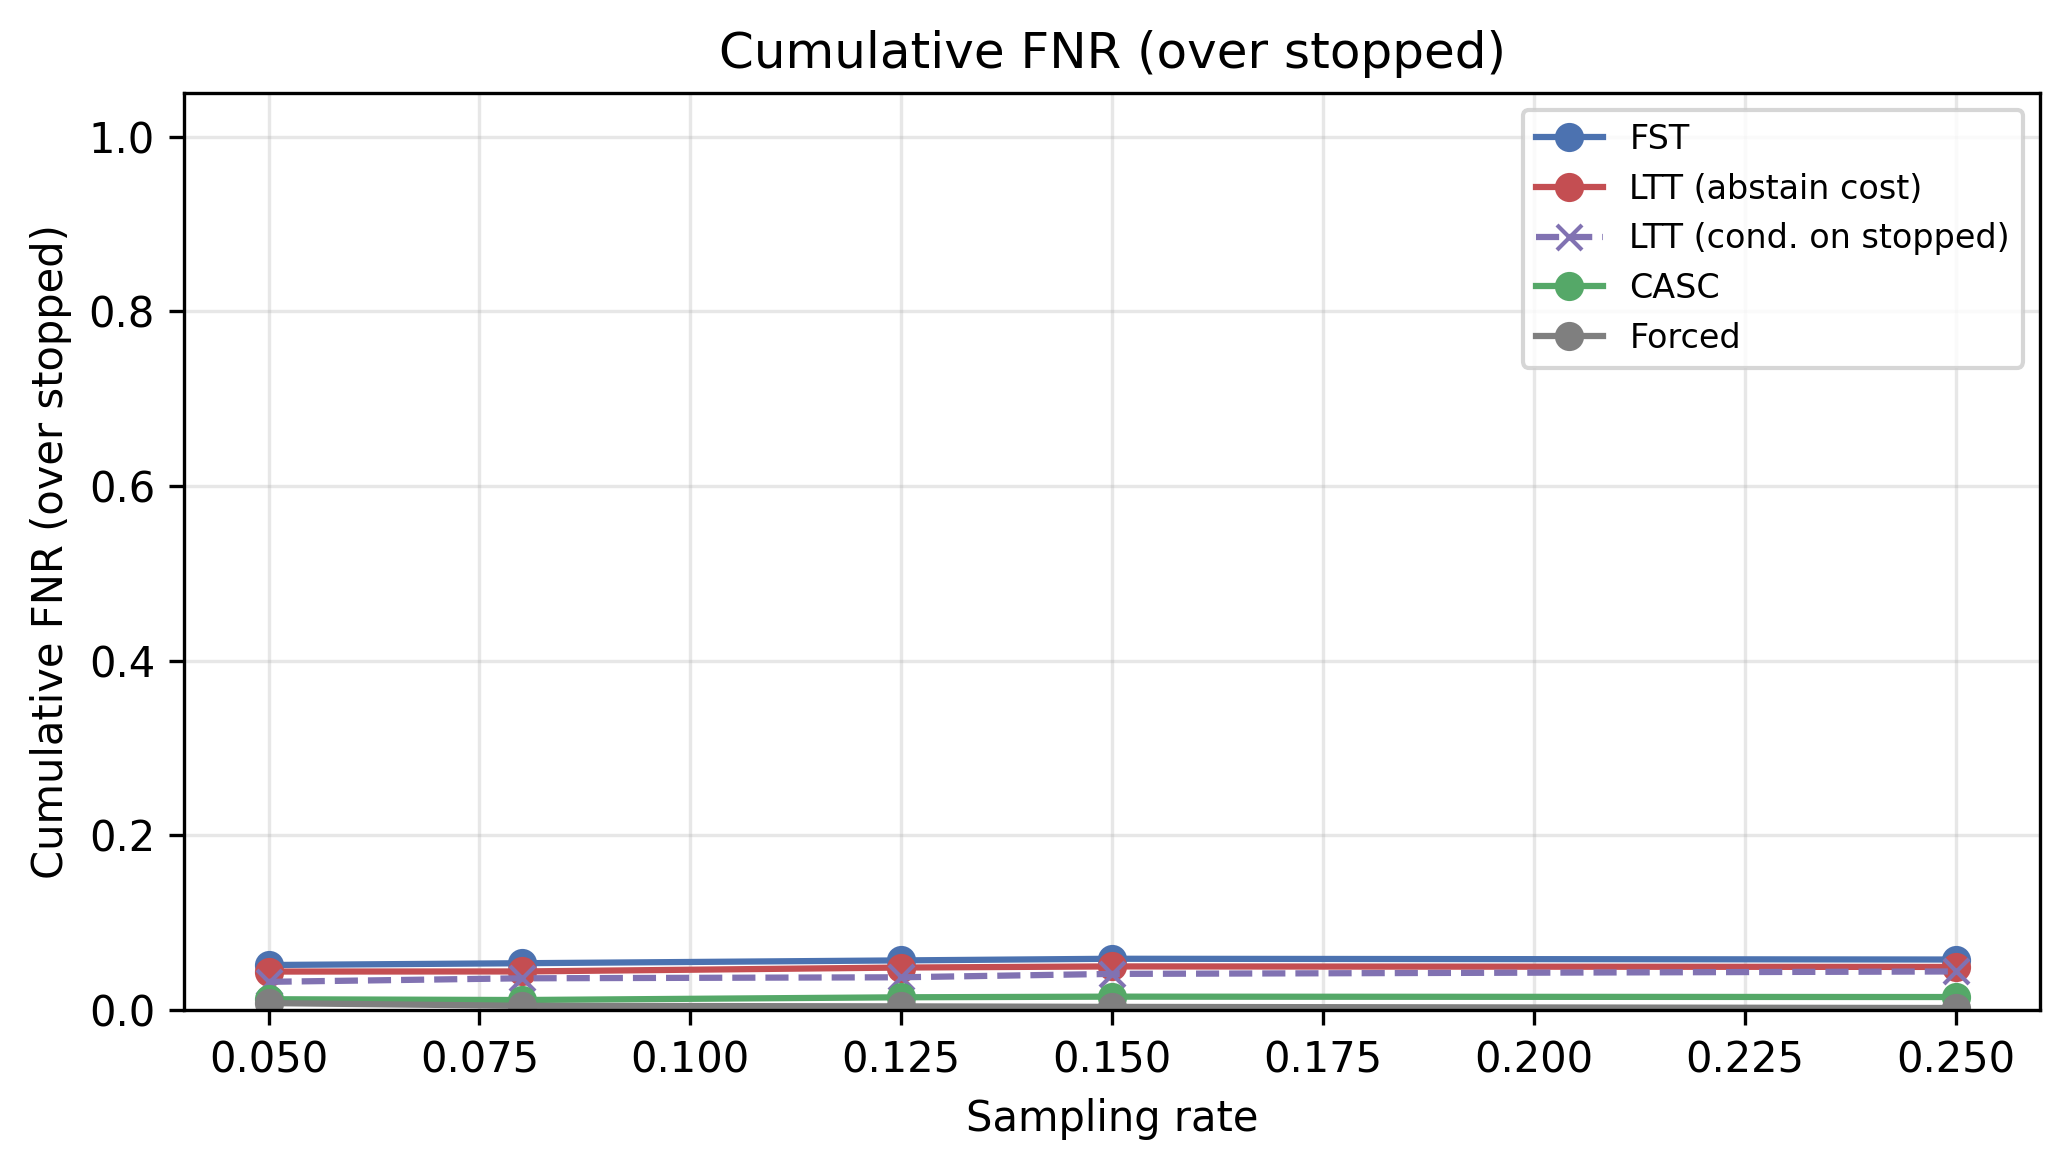
\includegraphics[width=\linewidth]{figures/knee_slice_compare_fnr_cumulative_vs_sampling_rate_knee_slice_fnr.png}
%         \caption*{(a) \textbf{FastMRI Knee Slices} : FNR among stopped samples against sampling rate}
%     \end{minipage}\hfill
%     \begin{minipage}{0.48\textwidth}
%         \centering
%         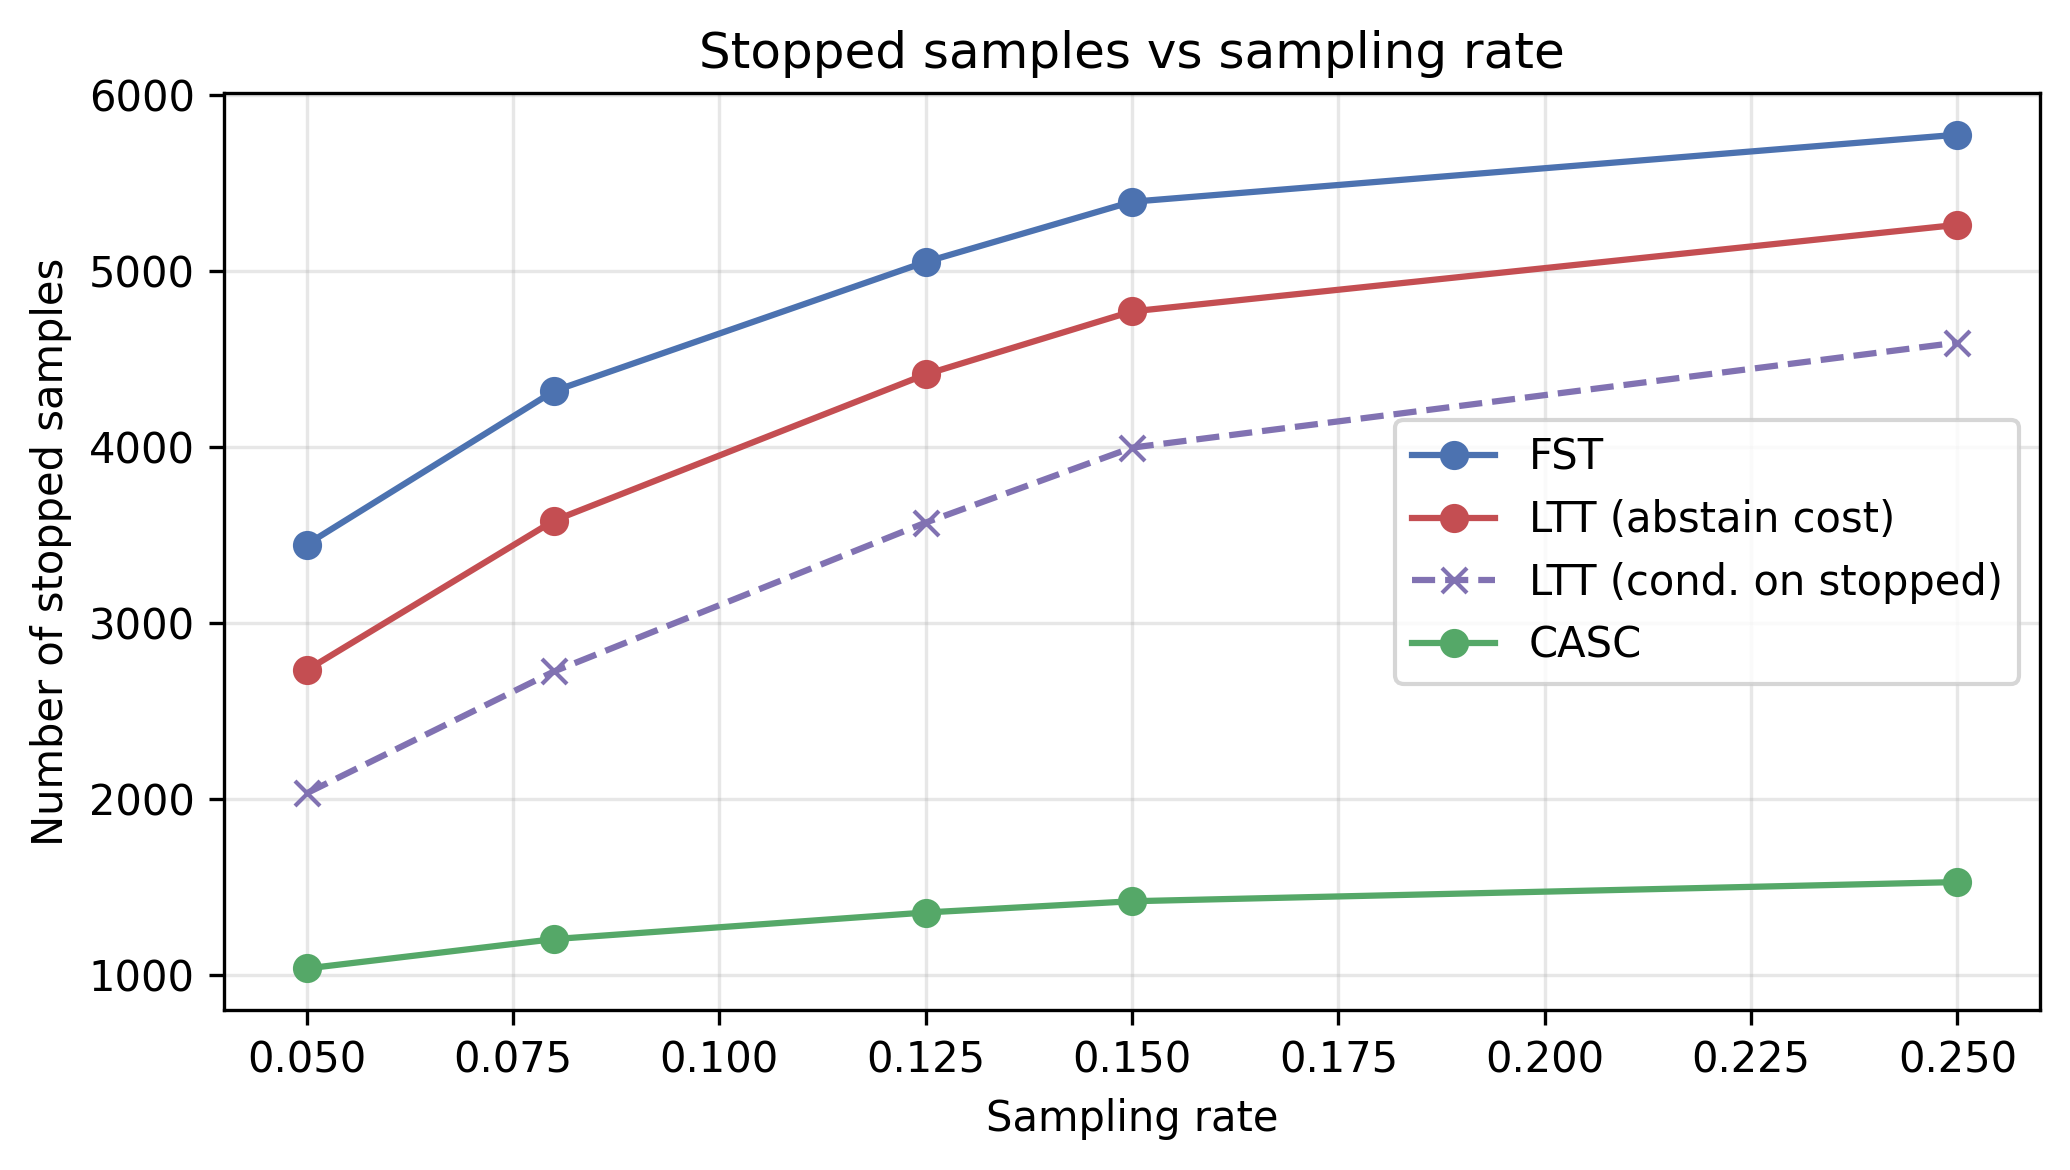
\includegraphics[width=\linewidth]{figures/knee_slice_compare_stopped_vs_sampling_rate_knee_slice_fnr.png}
%         \caption*{\textbf{FastMRI Knee Slices} : Fraction of stopped samples against sampling rate}
%     \end{minipage}
%     \caption{FastMRI Knee Slice-level Results}
%     \label{fig:two-plots}
% \end{figure}

% \begin{figure}[ht]
%     \centering
%     \begin{minipage}{0.48\textwidth}
%         \centering
%         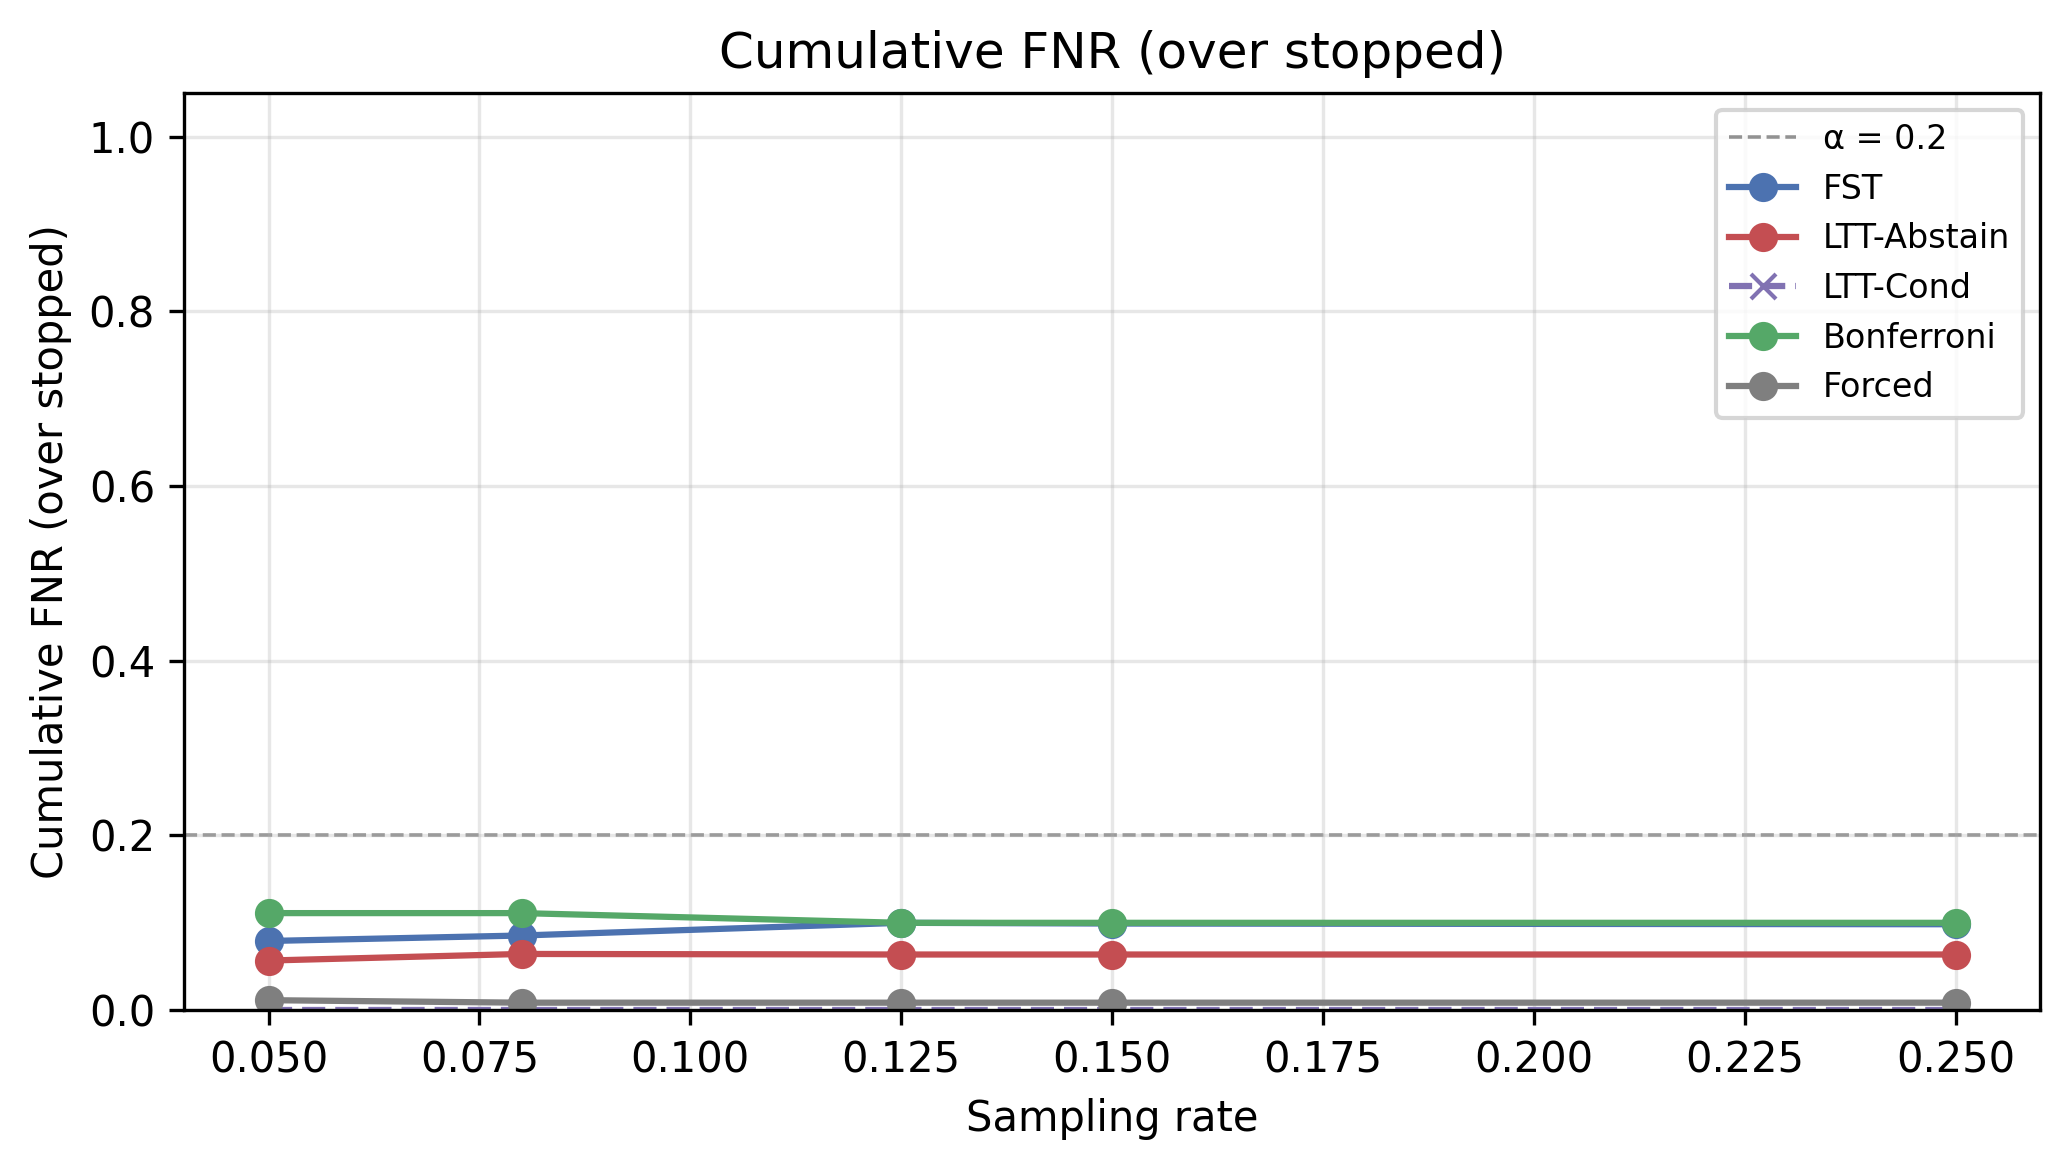
\includegraphics[width=\linewidth]{figures/knee_vol_asym_compare_fnr_cumulative_vs_sampling_rate_knee_vol_fnr_asym.png}
%         \caption*{(a) \textbf{FastMRI Knee Volumes} : Accuracy among stopped samples against sampling rate}
%     \end{minipage}\hfill
%     \begin{minipage}{0.48\textwidth}
%         \centering
%         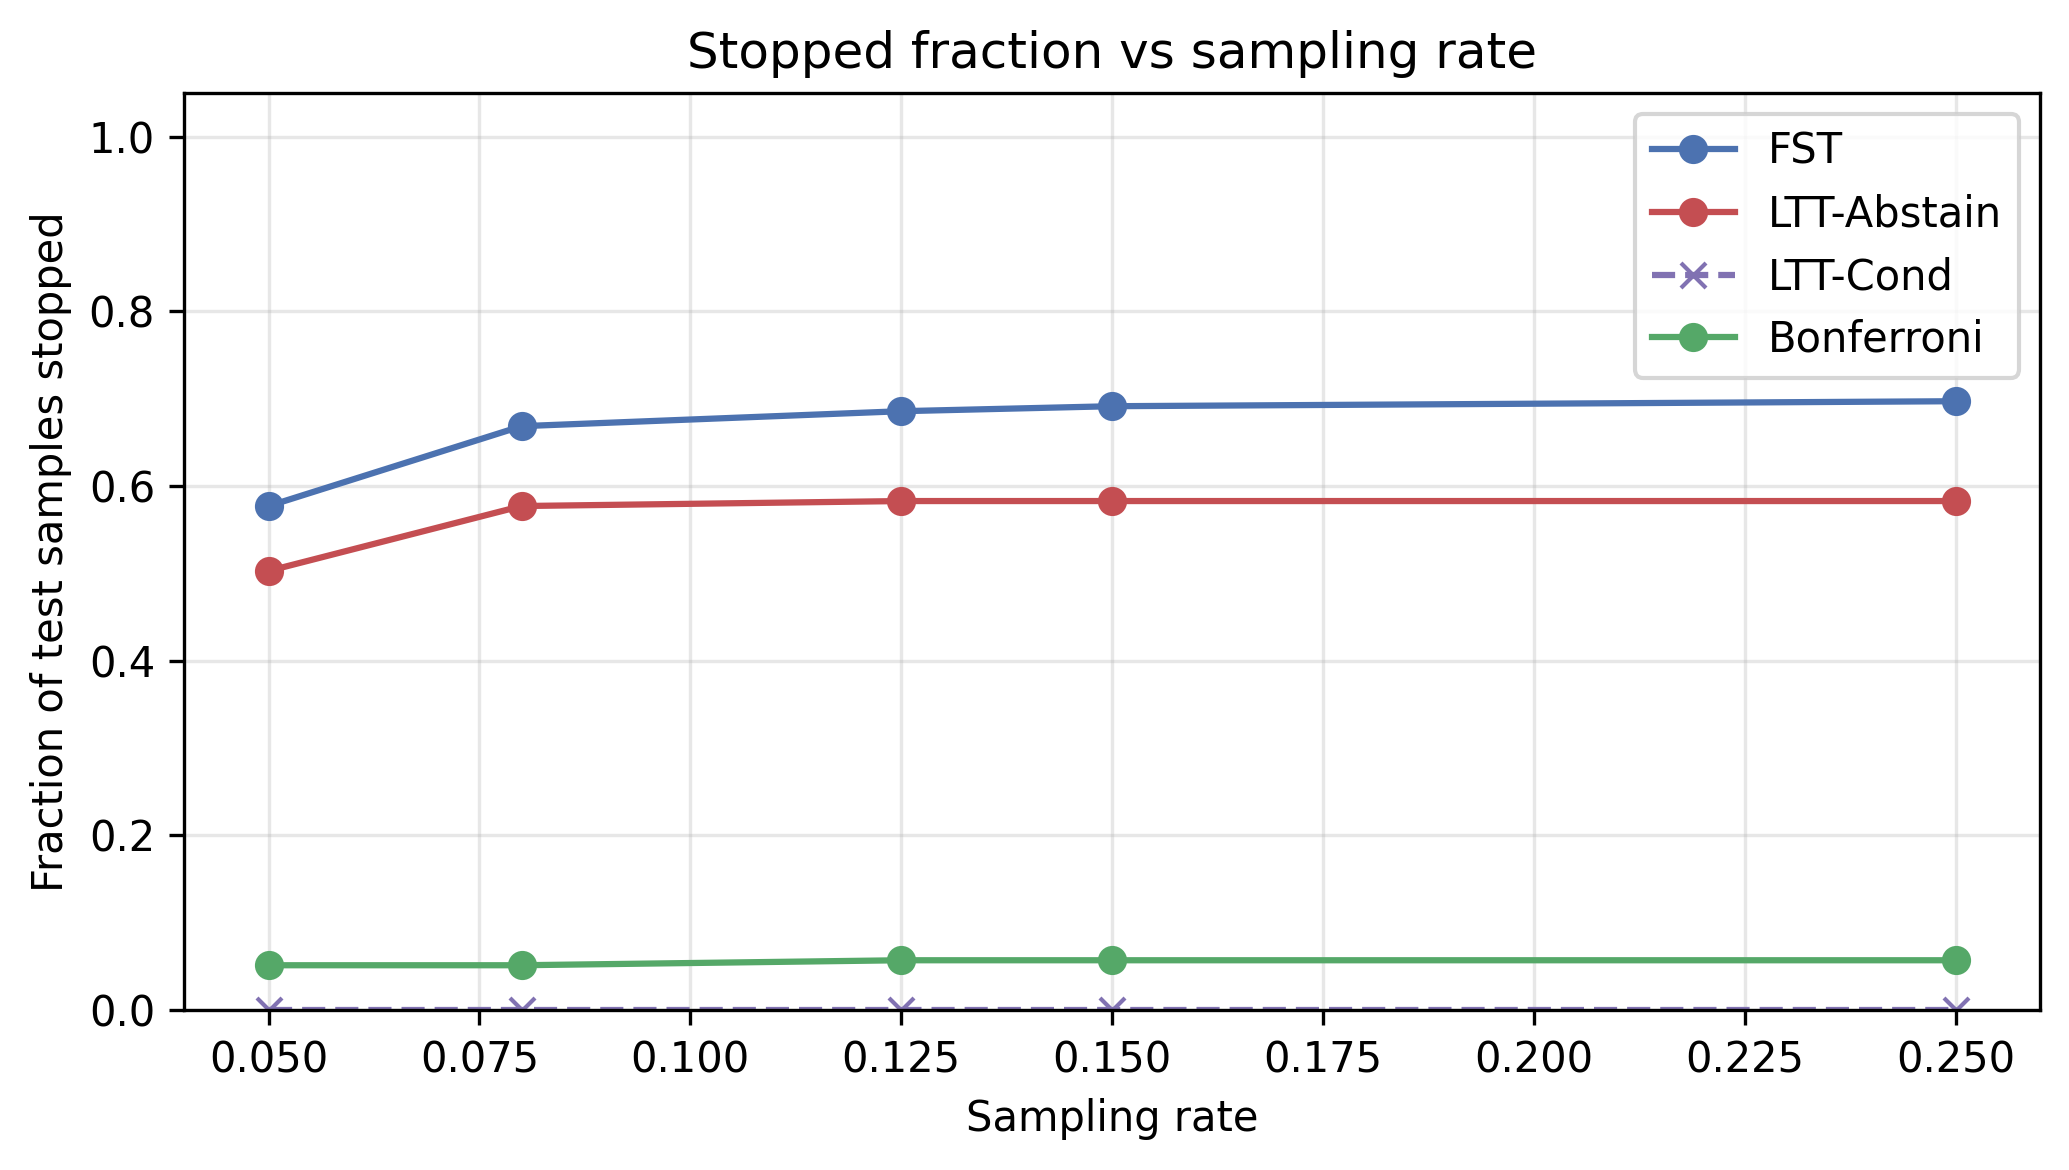
\includegraphics[width=\linewidth]{figures/knee_vol_asym_compare_stopped_vs_sampling_rate_knee_vol_fnr_asym.png}
%         \caption*{\textbf{FastMRI Knee Volumes} : Fraction of stopped samples against sampling rate}
%     \end{minipage}
%     \caption{FastMRI Knee Volume-Level Results}
%     \label{fig:two-plots}
% \end{figure}

% \begin{figure}[ht]
%     \centering
%     \begin{minipage}{0.48\textwidth}
%         \centering
%         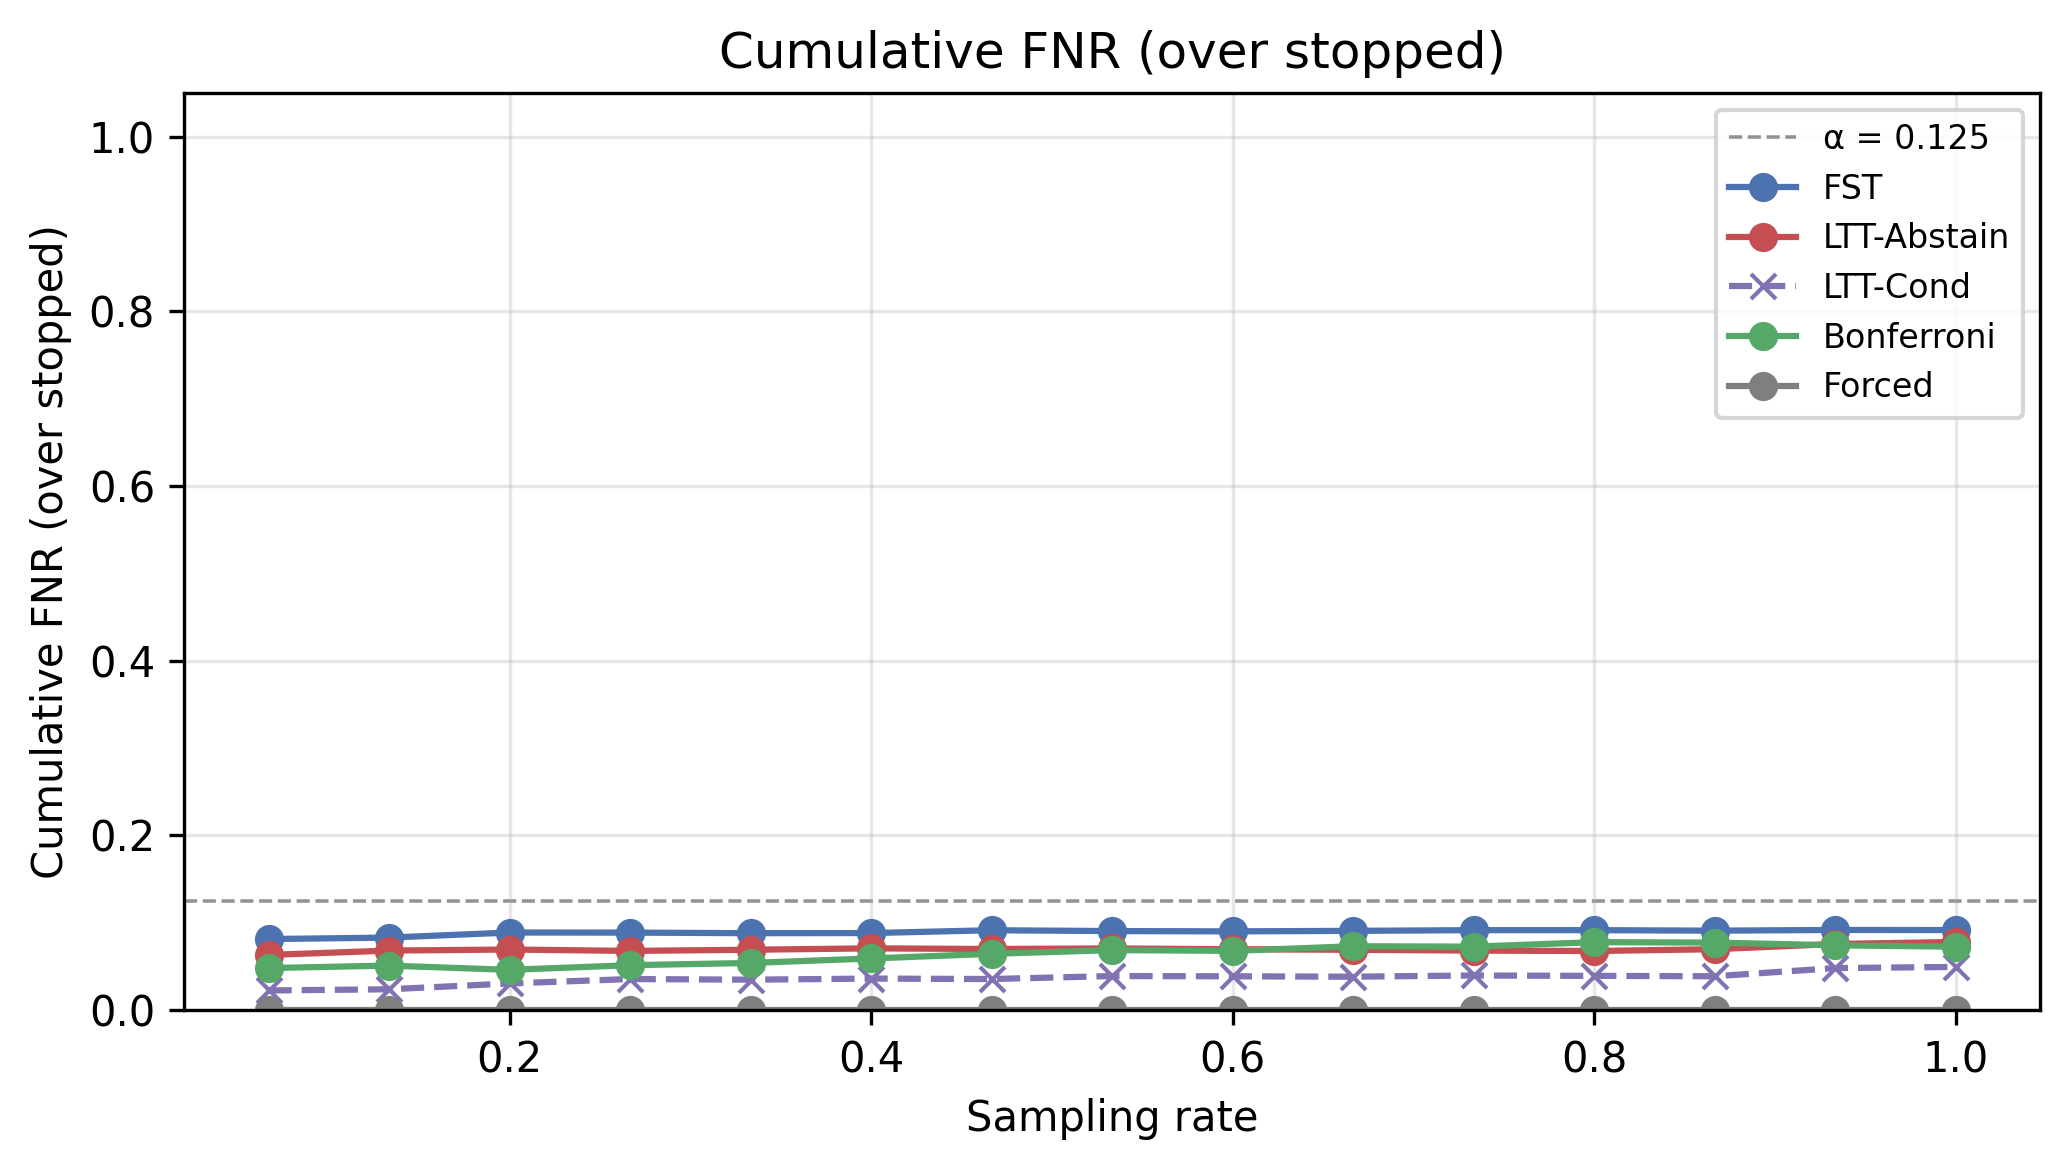
\includegraphics[width=\linewidth]{figures/prostate_asym_compare_fnr_cumulative_vs_sampling_rate_prostate_pirads_fnr_asym.png}
%         \caption*{(a) \textbf{Prostate} : Accuracy among stopped samples against sampling rate}
%     \end{minipage}\hfill
%     \begin{minipage}{0.48\textwidth}
%         \centering
%         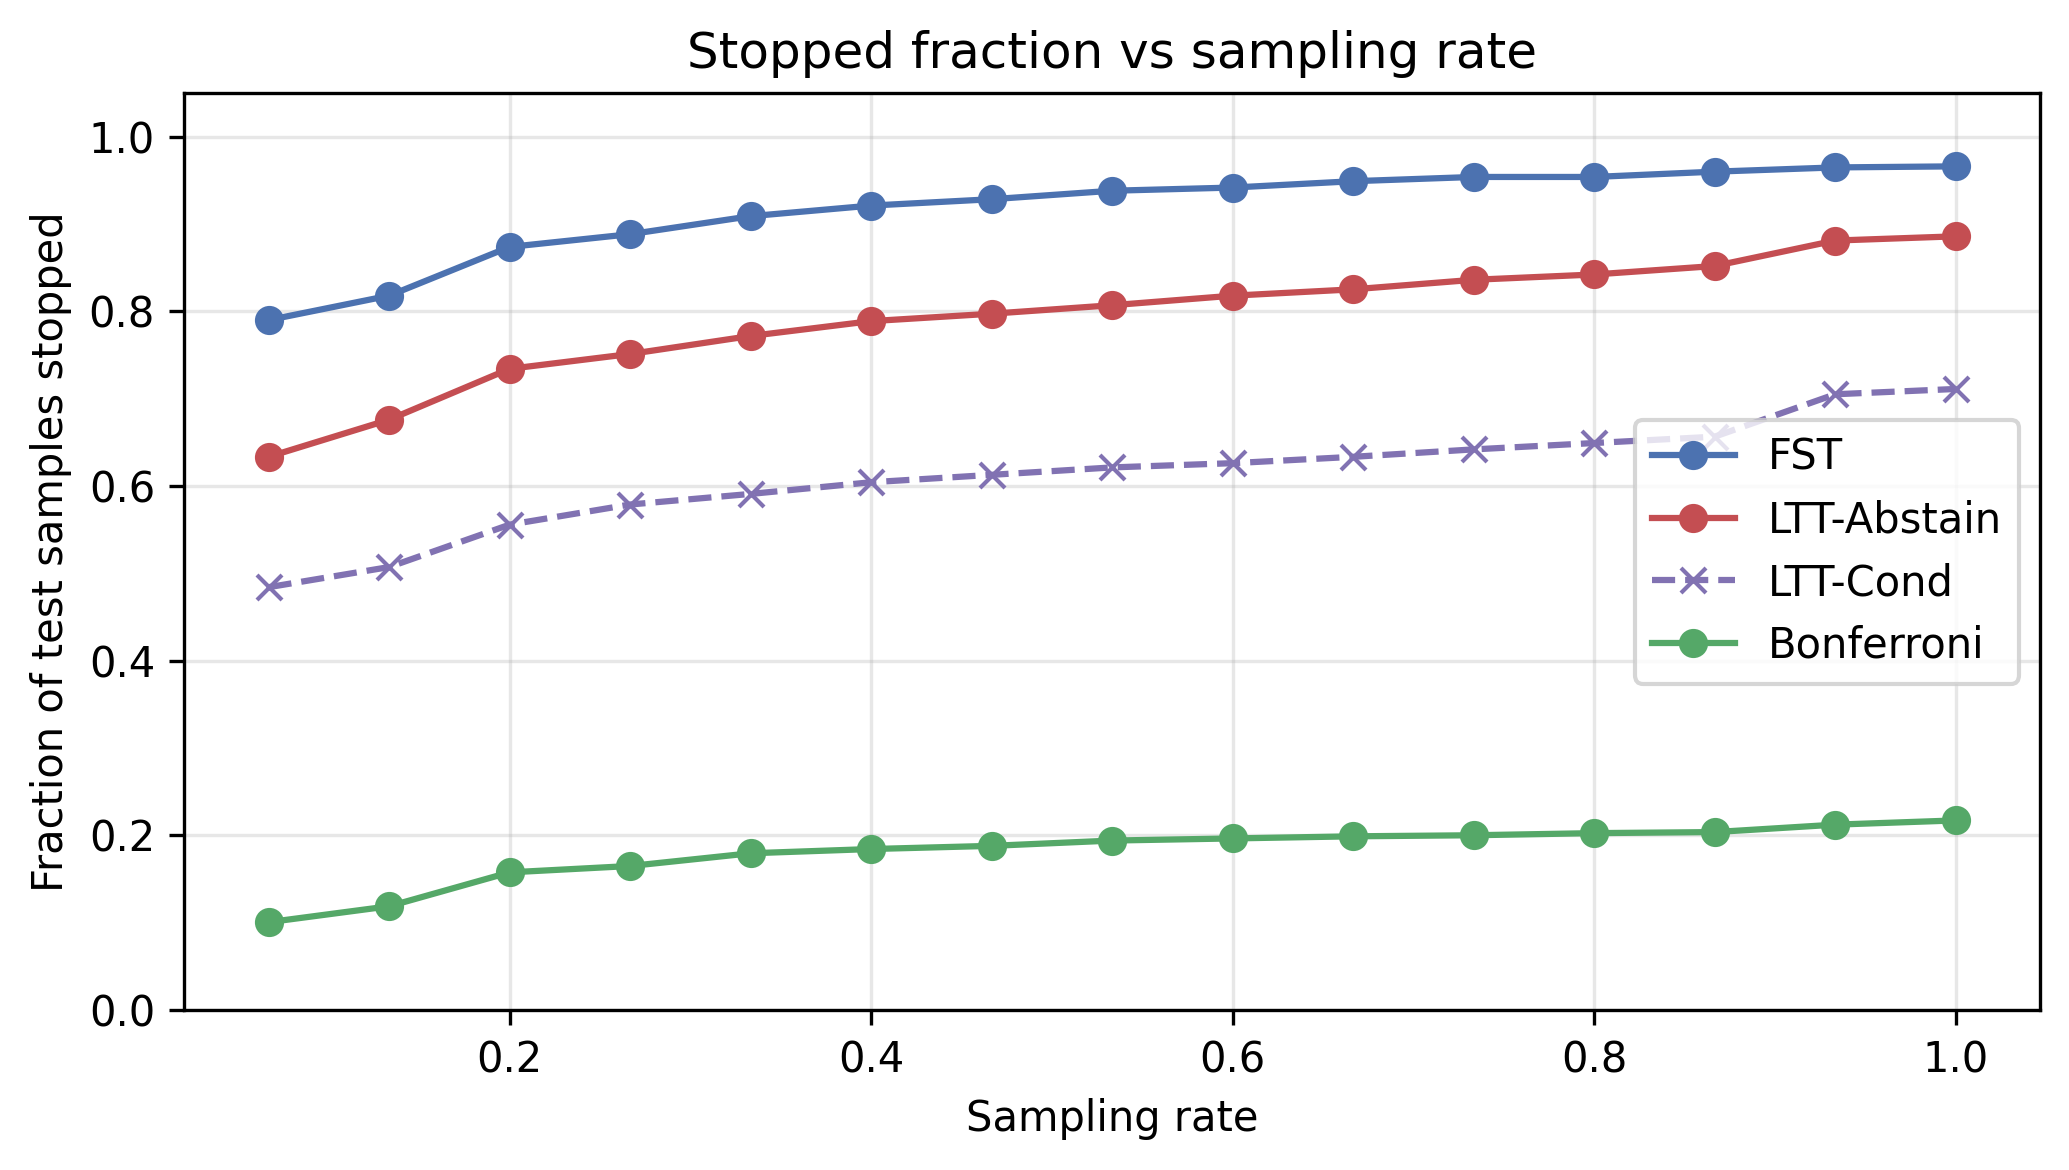
\includegraphics[width=\linewidth]{figures/prostate_asym_compare_stopped_vs_sampling_rate_prostate_pirads_fnr_asym.png}
%         \caption*{\textbf{Prostate} : Fraction of stopped samples against sampling rate}
%     \end{minipage}
%     \caption{FastMRI Prostate Results}
%     \label{fig:two-plots}
% \end{figure}


\subsection{Ambiguity-Band Stopping Policies}
\label{app:ambiguity_bands}

The \gls{method} procedure is agnostic to the form of the stopping policy $D_\lambda$, provided that the policy family is fixed prior to calibration and yields a bounded trajectory-level loss. In practice, however, the efficiency of safe stopping depends strongly on how this policy family is parameterized. We therefore instantiate $D_\lambda$ using a family of \emph{ambiguity-band stopping rules} defined over time-dependent predictive scores. This construction is used primarily for the MRI experiments, where clinically relevant false negative and false positive tradeoffs make thresholded score bands a natural decision primitive.

\paragraph{Predictive scores.}
Suppose that at acquisition time $t\in\{0,\dots,T-1\}$, the model outputs a positive-class score $S_{i,t,k}\in[0,1]$ for sample $i$ and label $k$, based on the cumulative partial observation $X_i^t$. In the multi-task setting, $k\in\{1,\dots,K\}$. Larger values of $S_{i,t,k}$ indicate stronger evidence for the positive class.

\paragraph{Baseline ambiguity anchors.}
For each acquisition step $t$ and task $k$, we define a pair of nominal ambiguity anchors $b^-_{t,k}, b^+_{t,k}$, with $0\le b^-_{t,k}\le b^+_{t,k}\le 1$, that identify a region of the score space where the model is considered ambiguous. Intuitively, scores below $b^-_{t,k}$ provide evidence for a negative decision, while scores above $b^+_{t,k}$ provide evidence for a positive decision. The interval $[b^-_{t,k},\, b^+_{t,k}]$ therefore serves as a time-specific uncertainty band. In our experiments, these anchors are estimated from a small held-out estimation set by comparing the empirical score distributions of positive and negative examples at each acquisition step. Concretely, for a fixed $(t,k)$, let
\begin{align*}
S^+_{t,k}=\{S_{i,t,k}: y_{i,k}=1\},
\qquad
S^-_{t,k}=\{S_{i,t,k}: y_{i,k}=0\},
\end{align*}
denote the positive- and negative-class score collections. We then define the nominal ambiguity anchors as the narrowest non-inverted quantile bracket within a pre-specified quantile family, yielding a data-driven aggressive endpoint for the band family. Importantly, these anchors are not themselves claimed to be risk-calibrated; rather, they serve to define an ordered family of stopping policies, while the actual statistical guarantee is supplied downstream by the \gls{method} calibration procedure.

\paragraph{Band modulation by $\lambda$}
Given the nominal anchors $(b^-_{t,k}, b^+_{t,k})$, we define a one-parameter family of effective ambiguity bands indexed by $\lambda\in[0,1]$:
\begin{align}
\label{eq:sym_bands_main}
\ell_{t,k}(\lambda)=\lambda\, b^-_{t,k},
\qquad
u_{t,k}(\lambda)=\lambda\, b^+_{t,k} + (1-\lambda).
\end{align}
This construction interpolates between:
\begin{itemize}
    \item \textbf{maximal ambiguity} at $\lambda=0$, where $[\ell_{t,k}(\lambda),u_{t,k}(\lambda)]=[0,1]$, and
    \item the \textbf{nominal ambiguity band} at $\lambda=1$, where $[\ell_{t,k}(\lambda),u_{t,k}(\lambda)]=[b^-_{t,k},b^+_{t,k}]$
\end{itemize}
Larger values of $\lambda$ therefore correspond to narrower ambiguity bands and more aggressive stopping rules.


\paragraph{Stopping rule.}
For a fixed $\lambda$, the stopping rule halts acquisition at the first time all tasks simultaneously exit their ambiguity bands. Formally, define the stopping time
\begin{align*}
\tau_\lambda(X_i) &= \inf\left\{t\in\{0,\dots,T-1\}: \forall k,\;
                    S_{i,t,k}\notin [\ell_{t,k}(\lambda),u_{t,k}(\lambda)]\right\}
\end{align*}
If no such time exists, we set $\tau_\lambda(X_i)=\infty$ and allow the policy to abstain or defer to the terminal horizon, depending on the risk formulation under consideration.

\paragraph{Terminal prediction.}
The ambiguity band jointly determines both stopping and prediction. Acquisition continues while the score remains inside the effective ambiguity interval \([\ell_{tk}(\lambda),u_{tk}(\lambda)]\). Once the score exits this interval, the side of exit determines the terminal class label: scores below the lower boundary are assigned to the negative class, while scores above the upper boundary are assigned to the positive class. Thus, for a single task, the sequential policy is
\[
D_\lambda(X^t)=
\begin{cases}
0, & S_t(X^t)<\ell_t(\lambda),\\
1, & S_t(X^t)>u_t(\lambda),\\
\mathrm{CONTINUE}, & S_t(X^t)\in[\ell_t(\lambda),u_t(\lambda)].
\end{cases}
\]
In the multi-task setting, acquisition halts once every task has exited its corresponding ambiguity band, and the terminal label for each task is determined by the side on which its score exits. This yields a complete stopping-and-prediction policy $D_\lambda$, which can then be certified by the procedure in Section~\ref{sec:rcs}.

\paragraph{Interpretation.}
The ambiguity-band construction should be viewed as a practical policy-family parameterization rather than as the source of the final guarantee. The role of the nominal anchors is to define an aggressive score-space ambiguity template at each acquisition time, and the role of $\lambda$ is to control how aggressively that ambiguity region is shrunk. The final risk guarantee is not inherited from the bands themselves, but from the downstream calibration procedure applied to the resulting trajectory-level stopping policies.

\newpage
\subsection{Clinical Prostate MRI Acquisition States}
\begin{figure}[h]
\centering
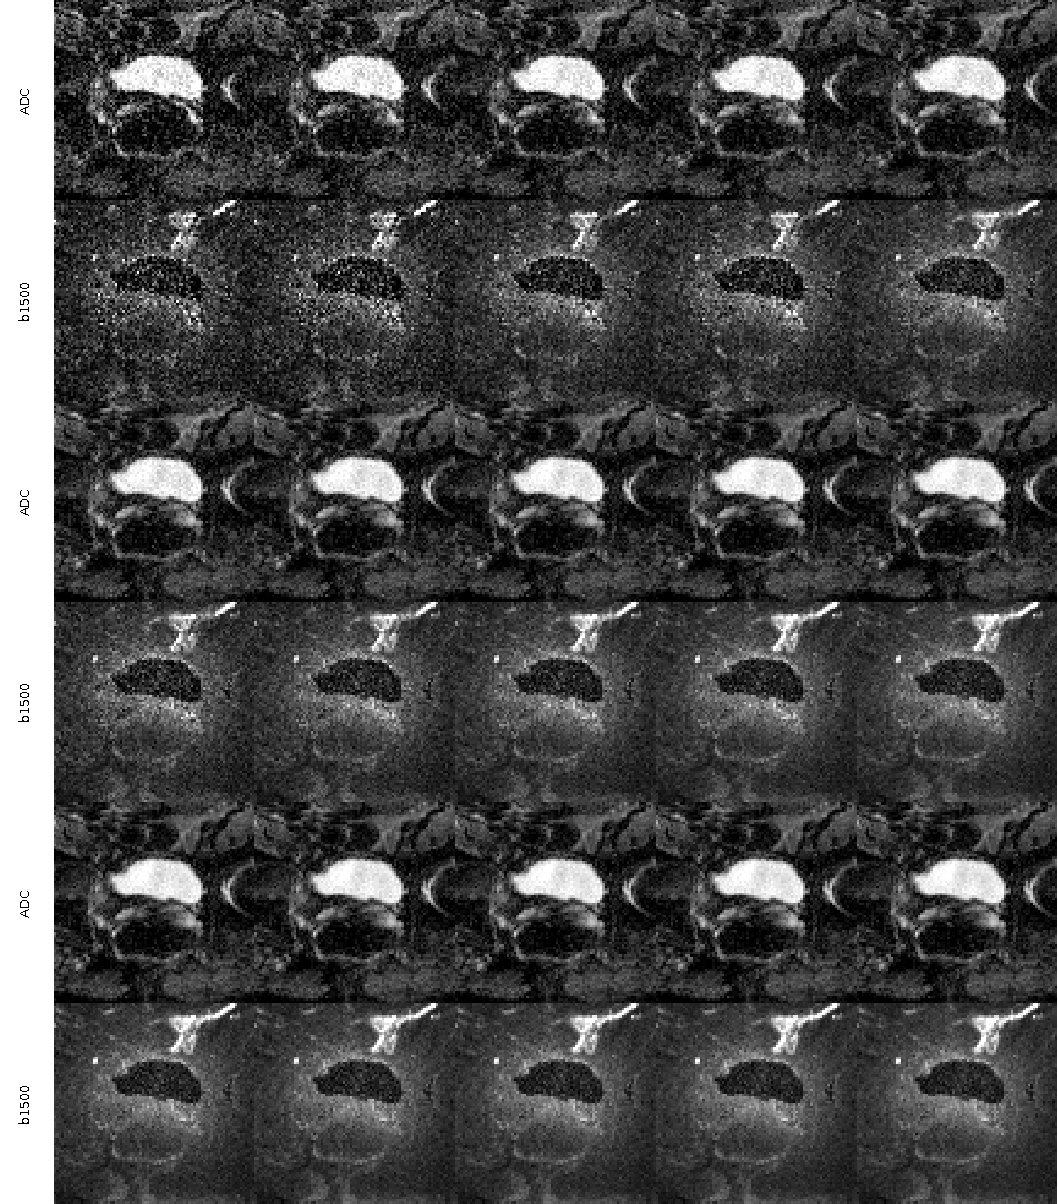
\includegraphics[width=\linewidth]{figures/prostate_dwi_acquisition_states_15.pdf}
\caption{Prostate DWI-derived images across sequential acquisition states.
Each tile shows ADC above computed high-b-value DWI ($b=1500$) for the same scan and slice.
Tiles are ordered left-to-right and top-to-bottom according to scanner acquisition order, from $1/1$ to $4/12$ acquired $b=50$/$b=1000$ averages.
}
\label{fig:prostate_dwi_acquisition_states}
\end{figure}

\end{document}
